\documentclass[]{article}
\usepackage{amsmath}\usepackage{amsfonts}
\usepackage[english]{babel}
\usepackage{amsthm}
\usepackage{listings}
\usepackage{courier}

\usepackage{fancyvrb}
\usepackage{beramono}
\usepackage{mathtools}
\usepackage{hyperref}

\usepackage[usenames,dvipsnames]{xcolor}
\usepackage[T1]{fontenc}
\usepackage[margin=1in,footskip=0.25in]{geometry}  % margin, foot skip
\usepackage[fontsize=12pt]{fontsize}
\usepackage[font=tiny]{caption}
\usepackage{subcaption}
\usepackage{wrapfig}
\usepackage{float}
\usepackage[final]{graphicx}


\lstset{basicstyle=\footnotesize\ttfamily,breaklines=true}
\newcommand{\indep}{\perp \!\!\! \perp}
\graphicspath{{.}}
\theoremstyle{definition}
\newtheorem{theorem}{Theorem}            % Theorem counter global 
\newtheorem{prop}{Proposition}[section]  % proposition counter is section
\newtheorem{lemma}{Lemma}[subsection]    % lemma counter is subsection
\newtheorem{definition}{Definition}      % theorem counter is global
\newtheorem{remark}{Remark}[subsection]  % remark counter is subsection
\hypersetup{
    colorlinks=true,
    linkcolor=blue,
    filecolor=magenta,
    urlcolor=cyan,
}
\urlstyle{same}
%%
%% Julia definition (c) 2014 Jubobs
%%

\lstdefinelanguage{Julia}%
  {morekeywords={abstract,break,case,catch,const,continue,do,else,elseif,%
      end,export,false,for,function,immutable,import,importall,if,in,%
      macro,module,otherwise,quote,return,switch,true,try,type,typealias,%
      using,while},%
   sensitive=true,%
   alsoother={$},%
   morecomment=[l]\#,%
   morecomment=[n]{\#=}{=\#},%
   morestring=[s]{"}{"},%
   morestring=[m]{'}{'},%
}[keywords,comments,strings]%

\lstset{%
    language         = Julia,
    basicstyle       = \ttfamily,
    keywordstyle     = \bfseries\color{blue},
    stringstyle      = \color{magenta},
    commentstyle     = \color{ForestGreen},
    showstringspaces = false,
}

\usepackage{setspace}
% \linespread{1}  % double spaced or single spaced

% For bibliography 
\usepackage{biblatex}
\addbibresource{refs.bib}

% for appendices
\usepackage[toc,page]{appendix}


\begin{document}
% important settings for hyperref counter and displayed counter. 
\numberwithin{equation}{subsection}
\numberwithin{figure}{subsection}
\counterwithin*{figure}{subsection}
\pagenumbering{gobble} % disable page number

% TITLE PAGE
\begin{center}
    \vspace*{1cm}
    Lanczos Algorithm and Conjugate Gradient
        
    \vspace{1.5cm}

    Hongda Li

    \vspace{0.8cm}
         
    submitted in partial fulfillment of the \\[1em]
    requirements for the degree of\\[1em]
    \vspace{1.5cm}
    Master of Science (Applied Mathematics)
         
    \vspace{0.8cm}
         
    

    University of Washington\\[1em]
    2022\\[1em]
    \vspace{1.5cm}
    Committee:\\[1em]
    name 1\\[1em]
    name 2\\
    \vspace{1.5em}
    Program Authorized to Offer Degree:\\[1em]
    Applied Mathematics
    

\end{center}
\newpage
\ % Copy right page don't know what to write. 
\newpage
\begin{center}
    University of Washington\\[1.5cm]
    \textbf{Abstract}\\[1.5cm]
    Lanczos Algorithm and Conjugate Gradient\\[2em]
    Hongda Li\\[2em]
    Chair of the Supervisory Committee:\\[0.5em]
    Name of the Committee Chair: \\[0.5em]
    Chair's Department
    
    
\end{center}
    \begin{spacing}{2}
    We review results from the literature on the conjugate gradient algorithm for solving symmetric positive definite linear systems and the related Lanczos algorithm.  We derive the conjugate gradient algorithm from the more general conjugate direction method, using projectors.  We establish error bounds using exact arithmetic theory and also discuss what can happen when floating point arithmetic is used.  We present numerical experiments to illustrate this behavior.
    \end{spacing}
\newpage

\pagenumbering{arabic} % enable page number
\tableofcontents

\newpage 


\section{Notations}
    \begin{enumerate}
        \item $\text{ran}(A):=\{Ax :\forall x \; \in \mathbb R^n\}, A \in \mathbb R^{m\times n}$, The range of a matrix. 
        \item $(A)_{i, j}$: The element in ith row and jth column of the matrix $A$.
        \item $(A)_{i:i', j:j'}$: The submatrix whose top left corner is the $(i, j)$ element in matrix $A$, and whose' right bottom corner is the $(i', j ')$ element in the matrix $A$. The notation is similar to MATLAB's rules for indexing. 
        \item $\forall\; 0\le j \le k$: under certain context it indicates the range for an index: $j = 0, 1, \cdots, k-1, k$
        \item Boldface $\mathbf 0$ denotes the zero vector or matrix, depending on the context it can be either a zero row/column vector, or a zero matrix.
        \item The $\hat{}$ decorator is reserved for denoting the unit vector of some non zero vector. For example $\hat{x}:= x/\Vert x\Vert, x \neq \mathbf 0$. 
        \item $p_k(A|w)$ denotes the matrix polynomial $\sum_{j = 0}^k w_jA^j$. 
        \item $\xi_i$ are used for the $i$ standard basis vector, the size of the vector depends on the context, sometimes it's denoted without ambguity for example: $\xi_i^{(k)}$ would denote the $i$ th standard basis vector for $\mathbb R^k$. 
    \end{enumerate}

\section{Introduction}
    The Conjugate Gradient method is an iterative method used for solving symmetric positive definite linear systems. It dates back to the period when computers were programmed using punched cards. It didn't receive much attention at the start but was revised and reappeared as a method for solving large sparse linear systems decades later, becoming the best option for positive definite linear systems that are sparse and large and, by extension, for optimizing strongly convex functions as well. In this thesis, we discuss the Conjugate Gradient method without pre-conditioning by deriving it and analyzing it along with the Lanczos algorithm, a closely related algorithm for solving symmetric eigenproblems. Finally, we use their connections to analyze their behaviors under floating-point arithmetic. The thesis will require some background in numerical linear algebra for the best understanding. 
    \par
    %In the first section, we introduce the projectors and Krylov subspace as important mathematical objects %for the subspace projections method, the frameworks for subspace projection methods, and the Lanczos %Iteration as a symmetric case of the Arnoldi Iterations. At the end of the section, we proceed and %derive the conjugate gradient method using only these ideas and concepts. In the second section, we %analyze the behaviors of Conjugate gradient and Lanczos Iterations, including the termination conditions %for both algorithms, their convergence rate, and the equivalence between them. The goal is to show how %they can be the same and have similar properties and how the connections between them can spark other %methods for solving a symmetric indefinite linear system. And in the final parts of the second section, %we derive the convergence bound for the conjugate gradient algorithm.
    In the first section, we introduce projectors and subspace projection methods.  We then specialize to Krylov subspaces and demonstrate that the conjugate gradient method can be thought of as producing an oblique projection onto a Krylov subspace.  We also derive the Lanczos algorithm as the symmetric version of the more general Arnoldi algorithm.  In the second section, we establish the well-known relationship between these two algorithms and we derive bounds on the convergence rate of the conjugate gradient algorithm.  In the third section, we use numerical experiments to better understand the algorithm behaviors under floating-point arithmetic, and we discuss possible ways to mitigate the effects of floating-point arithmetic, as well as what to expect if these effects are not mitigated.
    %\par
    %In the third section, we use numerical experiments to better understand the algorithm behaviors under %floating-point arithmetic. We show how floating-point arithmetic affects the Lanczos algorithm more %rigorously and how it may be fixed and mitigated, consequently improving the conjugate gradient %algorithm. 

\newpage
\begin{center}\large
    \textbf{Acknowledgement}
\end{center}

Thanks to Professor Greenbaum for taking the time to review the first draft of this thesis and for her help with my research throughout the year. Thanks to my old undergraduate classmate and friend who helped with fixing the typos on the later drafts. Thanks to the NARC reading group and participants at UW Applied Mathematics attend a trial run of the presentation for the content of this thesis. 



\newpage
\section{Foundations}
    In this section, we go over the foundations of the Conjugate Gradient and the Lanczos algorithms. We introduce the important ideas at the beginning, and then we proceed to derive the conjugate gradient algorithm from the method of conjugate directions.  We then derive the Lanczos algorithm as a symmetric case of the Arnoldi iteration. 
    \subsection{The Basics}
        In this subsection, we go over some basic concepts and mathematical entities that are important to Subspace Projection methods in general. 
        \subsubsection{Krylov Subspace}
            \begin{definition}[Krylov Subspace]
                $$
                \mathcal{K}_k(A|b) = \text{span}( b, Ab, A^2b, \cdots A^{k - 1}b)
                $$
                Observe that every element in the subspace is the product of a matrix polynomial with the vector $b$; we write it as $p_{k-1}(A|w)b$, where $p_{k-1}$ is a $(k-1 )^{st}$ degree  polynomial and $w$ is a vector denoting the coefficients. 
            \end{definition}
            \begin{definition}[The Grade of Krylov Subspace]
                The grade of the Krylov subspace for matrix $A$ and vector $b$ is $k - 1$ where $k$ is the smallest $k$ such that the vectors in $\mathcal K_{k}(A|b)$ are linearly dependent.  This will be denoted as $\text{grade}(A|b)$. Alternatively, it is also the degree of the minimal polynomial $p(A)$ such that $p(A)b= \mathbf 0$ .
            \end{definition}
            The terminology ``grade of a Krylov subspace'' is used in Y. Saad's work\cite{book:saad_sparse_linear}.
            Once the grade is reached, the Krylov subspace becomes an invariant subspace for the matrix $A$. For a proof, see \hyperref[prop:Krylov_Subspace_Grade_Invariant_Theorem]{Krylov Subspace Grade Invariant Theorem (\ref*{prop:Krylov_Subspace_Grade_Invariant_Theorem})} in the appendix. 
            \begin{prop}[When the Grade is Reached]\label{prop:When_the_Grade_is_Reached}
                Assuming that matrix $A$ is diagonalizable, $A = V\Lambda V^{-1}$, then $\text{grade}(A|u)$ is the number of unique $\lambda_i$ such that $(V^{-1}u)_i$ is non-zero. 
            \end{prop}
            \begin{proof}
                Let $\mathcal{K}_{k + 1}(A|u)$ be linearly dependent, then there is a nonzero vector $w$ such that: 
                %then it's the minimum number such that the matrix polynomial of $A$ multiplied by $u$ equals the zero vector, and %it's nontrivial. 
                \begin{align}
                    & \mathbf 0 = \sum_{j = 0}^{k}
                    w_jA^{j}u
                    \\
                    & \mathbf 0 = V\sum_{j = 0}^{k} w_j\Lambda^jV^{-1}u
                    \\
                    \forall i \quad 0 &= \left(
                            \sum_{j = 0}^{k} w_j\lambda_i^{j}
                        \right)(V^{-1}u)_i
                \end{align}
                It follows that $\sum_{j=0}^k w_j \lambda_i^j = 0$ whenever $( V^{-1} u )_i \neq 0$.
                If there are more than $k$ indices $i$, corresponding to distinct eigenvalues $\lambda_i$, for which $( V^{-1} u )_i \neq 0$, then the only vector $w$ for which the above equations will be satisfied is $w = \mathbf{0}$.  This is because the $k+1$ by $k+1$ matrix whose $(i,j+1)$ entry is $\lambda_i^j$ is a Vandermonde matrix and hence is nonsingular. However, if there are $k$ such indices $i$, then there will be a nonzero vector $w$ that satisfies the above $k$ equations in the $k+1$ unknowns, $w_0 , \ldots , w_k$.  If there are fewer than $k$ nonzero entries of $( V^{-1} u )_i$ corresponding to distinct eigenvalues $\lambda_i$, then, by the same arguments, the grade  will be less than $k$. 
                %When a non-trivial solution exists for some $w_j \neq 0$, then a polynomial will have to interpolate %$\lambda_i$ where $(V^{-1}u)_i\neq 0$. Therefore, the minimum $k$ is the number of unique $\lambda_i$ %such that $(V^{-1}u)_i\neq 0$
            \end{proof}
            
        \subsubsection{Projectors}
            \begin{definition}
                A matrix $P$ is a projector when $P^2 = P$, we call this property idempotent. 
            \end{definition}
            There are two types of projectors, oblique and orthogonal projectors. A projector is an orthogonal projector when it's Hermitian and oblique when it's not Hermitian. 
            \begin{prop}[Projector Complementary]
                The projector $I - P$ projects onto the null space of $P$ and vice versa. 
                \begin{align}
                    & \text{ran}(P) = \text{null}(I - P)
                    \\
                    & \text{ran}(I - P) = \text{null}(P)
                \end{align}
            \end{prop}
            The proof is immediate from the definition. For more coverage of facts, refer to Trefethen's Book on Numerical Linear Algebra\cite{book:trefethen}.

    \subsection{Subspace Projection Methods}\label{sec:Subspace_Projection_Methods}
        Let $\mathcal K, \mathcal L$ be two subspaces of $\mathbb{R}^n$. We will choose approximate solutions to our linear system $Ax=b$ from $\mathcal{K}$, and we will orthogonalize the residual $b-A \tilde{x}$ against $\mathcal{L}$.
        % $\mathcal K$ can be viewed as a subspace where we choose our solutions for the $x$ for the linear system $Ax = b$, 
        % and $\mathcal L$ is a subspace where we orthogonalize our residual $r = b - Ax$ against $\mathcal L$. 
        This is a description of this framework: 
        \begin{align}
            \text{choose }\tilde{x} \in x_0 + \mathcal{K} \text{ s.t: } b - A\tilde{x} \perp \mathcal{L} .
        \end{align}
        Let the columns of $V \in \mathbb{R}^{n \times m}$ be a basis for $\mathcal{K}$ and let the columns of $W \in \mathbb{R}^{n \times m}$ be a basis for $\mathcal{L}$.  Then
        % We look for a $\tilde x$ in the affine linear subspace $x_0 + \mathcal{K}$ such that it's perpendicular to the %subspace $\mathcal{L}$, or, equivalently, minimizing the projection onto the subspace $\mathcal{L}$. The above %conditions can be expressed using matrix. 
        % \begin{align}
        %        \text{Let } V \in \mathbb{R}^{n\times m} \text{ be a basis for: }\mathcal{K}
        %        \\
        %        \text{Let } W \in \mathbb{R}^{n\times m} \text{ be a basis for: } \mathcal{L}
        %    \end{align}
        %    Substituting the matrices to the above set of conditions: 
        \begin{align}\label{eqn.Orthogonalitycond}
            \tilde{x} &= x_0 + Vy
            \\
            \text{choose } x \text{ s.t: } b - A\tilde{x}  &\perp \text{ran}(W)
            \\
            \implies W^T(b - Ax_0 - AVy) &= \mathbf{0}
            \\
            W^Tr_0 - W^TAVy&= \mathbf{0}
            \\
            W^TAVy &= W^Tr_0
        \end{align}
        Thus we can determine the approximate solution $\tilde{x}$ by solving the linear system $W^T A V y = W^T r_0$ for $y$ (assuming that the matrix $W^T A V$ is nonsingular) and then setting $\tilde{x} = x_0 + V y$.  The new residual is
        $\tilde{r} = b - A \tilde{x} = b - A x_0 - AVy = r_0 - AV ( W^T A V )^{-1} W^T r_0$,
        and the matrix $AV ( W^T A V )^{-1} W^T$ is a projection since
        \begin{align}
            [ A V ( W^T A V )^{-1} W^T ] [ A V ( W^T A V )^{-1} W^T ] = A V ( W^T A V )^{-1} W^T
        \end{align}
        Alternatively, for some symmetric positive definite matrix $B$, one might choose $\tilde{x} = x_0 + Vy$ to minimize 
        the $B$-norm of the residual $\| r_0 - A V y \|_B = \langle r_0 - A V y , B ( r_0 - A V y ) \rangle^{1/2}$.  Setting the gradient of this function to zero leads to the normal equations:
        \begin{align}
            V^T A^T BAVy = V^T A^T B r_0
        \end{align}
        If $A$ itself is symmetric and positive definite, then we can take $B = A^{-1}$ and minimize the $A^{-1}$-norm of the 
        residual or, equivalently, the $A$-norm of the error $\langle A^{-1} b - \tilde{x} , A ( A^{-1} b - \tilde{x} ) \rangle$.
        The formula for $y$ then becomes
        \begin{align}\label{eqn:Energy_Norm_Minimization_Conditions}
            V^T A V y = V^T r_0
        \end{align}
        This is what the conjugate gradient algorithm does, taking the columns of $V$ to be an orthonormal basis of the Krylov space $\mathcal{K} = \mathcal{K}(A|b)$.  Note that this also involves a projection but the two spaces $\mathcal{K}$ and $\mathcal{L}$ and their bases $V$ and $W$ described above, are the same. Now
        \begin{align}
            \tilde{r} &= b - A \tilde{x}
            \\
            &= b - A x_0 - A V y
            \\
            &= r_0 - A V ( V^T A V )^{-1} V^T r_0
        \end{align}
        and the matrix $A V ( V^T A V )^{-1} V^T$ satisfies
        \begin{align}
            [A V (V^T A V )^{-1} V^T ] [ A V ( V^T A V )^{-1} V^T ] = A V ( V^T A V )^{-1} V^T
        \end{align}
        The $A$-norm of the error often represents energy in a mechanical system and so it is often referred to as the energy norm.
        
%        \subsubsection{Prototype Algorithm}
%           And from here, we can define a simple prototype algorithm using this framework. 
%            \begin{align}
%                \begin{aligned}
%                    & \text{While not converging}: 
%                    \\&\hspace{1.1em}
%                            \begin{aligned}
%                            &\text{Increase Span for: } \mathcal{K, L}
%                            \\
%                            &\text{Choose: } V, W \text{ for } \mathcal{K}, \mathcal{L}
%                            \\
%                            & y:= (W^TAV)^{-1}W^Tr_0
%                            \\
%                            & x:= x+ Vy
%                            \\
%                            & r:= r_0 - AVy
%                        \end{aligned}
%                \end{aligned}
%            \end{align}
%            Each time, we increase the span of the subspace $\mathcal K, \mathcal L$, which gives us more space to choose the %solution $x$, and more space to reduce the residual vector $r$. This idea is incredibly flexible, and we will see in a later %part that it reduces to a more concrete algorithm. Finally, when $\mathcal K = \mathcal L$, this is referred to as Petrov %Galerkin's Conditions (\textbf{TODO CHECK THIS}). 
%            \\
%            \begin{remark}[Projector in the Prototype Algorithm]
%                One may proceed to find a projector in the above prototype algorithm. 
%                \begin{align}
%                    & y = (W^TAv)^{-1}W^Tr_0
%                    \\
%                    & AVy = AV(W^TAV)^{-1}W^{T}r_0
%                    \\
%                    & x = x_0 + AVy
%                    \\
%                    & b - Ax = b - Ax_0 - AVy
%                    \\
%                    & r = r_0 - AV(W^TAV)^{-1}W^Tr_0
%                \end{align}
%                Here, $AV(W^TAV)^{-1}W^T$ is a projector, assuming the invertibility of $W^TAV$. 
%            \end{remark}
 \iffalse       
        \subsubsection{Energy Norm Minimization using Gradient}\label{sec:Energy_Norm_Minimization_using_Gradient}
            Other times, an iterative method will choose to build up a subspace for each step with a subspace generator, and build up the solution on this expanding subspace, but with the additional objective of minimizing the residual under some norm. Assuming that the vector $x\in x_0 + \mathcal{K}$, we want to minimize the residual under a norm induced by positive definite operator $B$. Let it be the case that the columns of matrix $K$ span subspace $\mathcal{K}$ with $\dim(\mathcal K) = k$, then one may consider using gradient as a more direct approach instead of projector. 
            \begin{align}
                &\hspace{0.6em} \min_{x\in x_0 + \mathcal{K}} \Vert b - Ax\Vert_B^2 
                \\
                &= \min_{w\in \mathbb{R}^{k}} 
                \Vert b - A(x_0 + Kw)\Vert_B^2 & 
                \\
                &= \min_{w\in \mathbb{R}^{k}} 
                \Vert 
                    r_0 - AKw
                \Vert_B^2
            \end{align}
            We take the derivative of it and set the derivative to zero to look for the minimum, skipping the proof that the derivative of $\nabla_x[\frac{1}{2}\Vert x\Vert_A^2] = Ax$ and just apply this formula for computing the gradient $\nabla_x[f(Ax)] = A^T\nabla_x [f(x)]$ where $f(x)$ is a mapping from $\mathbb R^n$ to $\mathbb R$. 
            \begin{align}
                \nabla_w \left[
                    \Vert r_0 - AKw\Vert_B^2
                \right] &= \mathbf{0}
                \\
                (AK)^TB(r_0 - AKw) &= \mathbf{0}
                \\
                (AK)^TBr_0 - (AK)^TBAKw &= \mathbf{0}
                \\
                (AK)^TBr_0 &= (AK)^TBAKw
            \end{align}
            The above formulation is powerful. We used gradient instead of projector for the simplicity of the argument. One can derive the same using an orthogonal projector to minimize the equivalent 2-norm of the energy norm, but the math is a bit more tedious. However, this minimization objective is minimizing the residual, which is fine for deriving subspace methods such as the GMRes, or the Minres and Orthomin, however, for the sake of the conjugate gradient, we have to consider the alternative. Let this be a proposition that we proceed to prove. 
            \begin{prop}[Conditions for Minimum Error Under Energy Norm]
                Here, we let matrix $B$ be positive definite so that it can induce a norm, we let $K$ be a matrix whose columns form a basis for $\mathcal K$, we let $e_k$ denotes the error, given by: $A^{-1}b - x_k$, and we let $r_k$ denotes the residual given as $b - Ax_k$. 
                \begin{align}
                    \min_{x_k\in x_0 + \mathcal K}\Vert A^{-1}b - x\Vert_B^2
                    \iff
                    K^TBe_0 - K^TBKw &= \mathbf 0
                \end{align} 
            \end{prop}
            Next, we proceed to prove it and explain its interpretations and importance: 
            \begin{proof}
                \begin{align}
                    \min_{x \in x_0 + \mathcal K}
                    \Vert A^{-1}b - x\Vert_B^2
                    &= 
                    \min_{x\in \mathbb R} 
                    \Vert A^{-1}b - x_0 - Kw\Vert_B^2
                    \\
                    &= \min_{x\in \mathbb R^k}
                    \Vert e_0 - Kw\Vert_B^2
                \end{align}
                To attain the minimum of the norm, we take the derivative and set it to be zero, giving us: 
                \begin{align}
                    \mathbf 0 &= \nabla_w[\Vert e_0 - Kw\Vert_B^2]
                    \\
                    &= \nabla_w[e_0 - Kw]^TB(e_k - Kw)
                    \\
                    &= 2K^TB(e_0 - Kw)
                    \\
                    \implies 
                    K^TBe_0 - K^TBKw &= \mathbf 0
                \end{align}
            \end{proof}
            This conditions (3.2.28) is implicitly describing the objective of a Preconditioned Conjugate Gradient algorithm, where $B$ is the $E^{-1}AE^{-T}$ matrix with $M = E^{-1}E^{-T}$ a symmetric positive definite matrix approximating the inverse of matrix $A$. Let's refrain from such a digression and instead let's set $B$ to $A$, so that it's equivalent to the Energy Norm minimization of Conjugate Gradient, giving us this condition: 
            \begin{align}
                K^TAA^{-1}r_0 - K^TAKw &= \mathbf 0
                \\
                K^Tr_0 - K^TAKw &= \mathbf 0
            \end{align}
            Here, we just made the substitution of $e_0 = A^{-1}r_0$, and $B = A$ to (3.2.28). Later, we will see how this condition is related to oblique Projector, similar to how an Orthogonal Projector is able to minimize the 2-Norm of the residual. 
\fi

    \subsection{Deriving Conjugate Gradient from Conjugate Directions}
        At the time this is being written, it's been 70 years since the Conjugate Gradient algorithm was proposed by Hestenes and Stiefel back in 1952\cite{paper:cg_original}. Upon their first discussion of the algorithm, numerous perspectives were explored. Three of the most important ideas are using Conjugate Directions, minimizing the energy norm of the error of the linear system and coming up with an update of the conjugate vectors using the residual vector at the current iteration. Here, we use the exact same idea, but we diverge from Hestenes and Stiefel's approach in favor of using the oblique projector and the subspace orthogonality conditions to derive it. The ideas are rehashed we point out its relations to Krylov Subspace only at the end. Usually under classroom settings or textbooks, the relations of Conjugate Gradient, Lanczos Iterations and Krylov Subspaces are discussed together to explain some of the more important properties of the algorithm so that we can move on and talk about other things. However, in this section we derive it in a way similar to the approach used in course notes by Shewchuk \cite{notes:painless_cg}. 
        \subsubsection{CG Objective and Framework}
            We introduce the algorithm as an attempt to minimize the energy norm of the error for a system of linear equations $Ax = b$, and we make the assumptions: 
            \begin{itemize}
                \item [1)] The matrix $A$ is symmetric positive definite.  
                \item [2)] There is a matrix $P_k = [p_0 \;p_1\;\cdots p_{k-1}]$ whose columns form a basis for the space over which we are minimizing.
            \end{itemize}
            Let's consider the following objective of minimizing the energy norm of the error over a subspace. 
            \begin{align}
                \min_{w \in \mathbb{R}^k}\Vert 
                    A^{-1}b - (x_0 + P_kw)
                \Vert_A^2 \iff P^T_kr_0 = P_k^TAP_kw
            \end{align}
            Refer back to \hyperref[eqn:Energy_Norm_Minimization_Conditions]{equation (\ref*{eqn:Energy_Norm_Minimization_Conditions})} for how to obtain the above condition. Using the matrix
            from \hyperref[eqn.Orthogonalitycond]{equation (\ref*{eqn.Orthogonalitycond})},
        %    from the \hyperref[sec:Subspace_Projection_Methods]{subspace projection method (\ref*{sec:Subspace_Projection_Methods})} 
            where $W, V$ are both $P_k$, we reformulate the norm minimization conditions as: 
            \begin{align}
                \text{choose: }x \in x_0 + \text{ran}(P_k) \text{ s.t: } b - Ax \perp \text{ran}(P_k)    
            \end{align}
            Take note that the link between a norm minimization and an equivalent subspace orthogonality condition isn't guaranteed to happen for other subspace projection methods. For example, the FOM and Bi-Lanczos Methods are orthogonalization methods that don't directly link to a norm minimization objective \cite{paper:FOM}. 
            \par
            To solve for $w$, we wish to make $P_k^TAP_k$ to be an easy-to-solve matrix. Let the easy-to-solve matrix be a diagonal matrix and hence we let $P_k$ be a \textit{matrix whose columns are A-Orthogonal vectors}. It's also referred to as \textit{conjugate vectors}. 
            \begin{align}
                P^T_kAP_k &= D_k \text{ where: } (D_k)_{i,i} = \langle p_{i - 1}, Ap_{i - 1}\rangle
                \\
                P_k^T r_0 &= P^T_kAP_kw = D_kw
                \\
                w &= D^{-1}_kP_k^Tr_0
            \end{align}
           % The idea here is: accumulate vectors $p_j$ into the matrix $P_k$ and then iteratively improve the solution $x_k$ by reducing the error denoted as $e_k$ defined as $A^{-1}b - x_k$. Then, we derive the following expression for $x_k$ and the residual $r_k = b - Ax_k$: 
           Now we have the following expressions for $x_k$ and $r_k$:
            \begin{align}
                \begin{cases}
                    x_k = x_0 + P_kD^{-1}_kP^T_kr_0
                    \\
                    r_k = r_0 - AP_kD^{-1}_kP^T_k r_0
                \end{cases}
            \end{align}
            Let this algorithm be the prototype. 
        \subsubsection{Using the Projector}
            Observe that $AP_kD_k^{-1}P_k$ is a projector, and so is $P_kD^{-1}_kP_k^TA$. We can check by: 
            \begin{align}
                AP_kD^{-1}_kP_k^T(AP_kD^{-1}_kP_k^T) 
                &= 
                AP_kD^{-1}_k
                    \underbrace{(P_k^TAP_k)}_{D_k}
                D^{-1}_kP_k^T  = AP_kD_k^{-1}P_k^T 
                \\
                P_kD^{-1}_k
                \underbrace{P_k^{T}A(P_k}_{D_k}
                D^{-1}_kP_k^{T}
                A) &= P_kD^{-1}_kD_kD_{k}^{-1}P^T_kA
                = P_kD^{-1}_kP^T_kA
            \end{align}
            \noindent
            They are not Hermitian,therefore they are oblique projectors. For convenience, we denote $\overline{P}_k = P_kD_k^{-1}P_k^{T}$; So we can simply denotes them by $A\overline{P}_k, \overline{P}_kA$. Observe that: 
            \begin{align}
                & \text{ran}(I - A\overline{P}_k )\perp \text{ran}(P_k)
                \\
                & \text{ran}(I - \overline{P}_kA) \perp \text{ran}(AP_k)
            \end{align}
            because:
            \begin{align}
                P_k^T(I - A\overline{P}_k) &= P_k^T - P_k^{T}A\overline{P}_k
                \\
                &= P_k^{T} - D_kD_k^{-1}P^T_k = \mathbf{0}
                \\
                (AP_k)^T(I - \overline{P}_kA) &=P_k^TA - P_k^TA\overline{P}_kA
                \\
                &= P_k^TA - P_k^TAP_kD_k^{-1}P_k^TA
                \\
                &= P_k^TA - P^T_kA = \mathbf{0}
            \end{align}
            
            
            \begin{prop}[Generating $A$-Orthogonal Vectors]
                Given any set of linearly independent vectors, for example $\{u_i\}_{i = 0}^{n - 1}$, one can generate a set of A-Orthogonal vectors from it. More specifically:
                \begin{align}
                    p_k &= (I - \overline{P}_kA)u_k \implies p_k \perp \text{ran}(AP_k)
                \end{align}
            \end{prop}
            \begin{proof}
                It's direct from the properties of the projectors.
            \end{proof}
            
        \subsubsection{Method of Conjugate Directions}
            So far, we have this particular scheme of solving the optimization problem, coupled with the way to compute the solution $x_k$ at each step, and the residual $r_k$ at each step.  However, it would be great if
            we could update $x_k$, $r_k$, and $p_k$ using results from previous iterations.
            %we can accumulate on the same subspace $P_k$ and look for a chance to reuse the computational results from the previous iterations of the algorithm: 
            \begin{definition}[Conjugate Direction Method]
                \begin{align}
                    \begin{cases}
                        \overline{P}_k = P_kD^{-1}_kP_k^T
                        \\
                        x_k = x_0 + \overline{P}_k r_0
                        \\
                        r_k = (I - A\overline{P}_k) r_0
                        \\
                        P^T_kAP_k = D_k
                        \\
                        p_k = (I - \overline{P}_kA)u_k & \{u_i\}_{i = 0}^{n - 1} \text{linearly independent vectors}
                    \end{cases}
                \end{align}
            \end{definition}
            With the assistance of a set of basis vectors that span the whole space, this algorithm can achieve the objective. 
            %Take note that we can accumulate the solution for $x_k$ accumulatively, instead of computing the whole projector process, we have the choice to update it recursively as the newest $p_k$ vector is introduced at that step. Let's Call this formulation of the algorithm: \textit{Conjugate Direction Method}(CDM). 
            \begin{remark}
                This CDM method is nothing new, in the original paper from Hestenes and Stiefel back in 1952\cite{paper:cg_original}, they commented on the method of Conjugate Direction, for each choice of basis $\{u_i\}_{i = 0}^{n-1}$ there is a unique algorithm. If one were to choose the basis to be the set of standard basis vectors, then the resulting algorithm would be the equivalent of  Gaussian Elimination. 
            \end{remark}
            \begin{remark}[Geometric Intuition of CDM]
                What is happening geometrically is that the A-Orthogonal vectors are orthogonal if described under the alternative eigenspace. Intuitively, one should think of a high-dimensional sphere that sits along some orthogonal basis, and the transformation of $A$ is stretching and rotating sphere, along with the orthogonal axis, resulting in a new ellipsoid in a different orientation; when the transformation is applied, the orthogonal coordinate inside the sphere got stretched along with it, and now these axes had become A-orthogonal vectors. Tracing along the direction of these vectors will ensure minimum redundancy of search directions. 
            \end{remark}
        \subsubsection{Properties of CDM}
            Here we set up several useful lemma and propositions that can derive the short recurrences of A-Orthogonal vectors 
            \begin{prop}[CDM Property 1]
                \begin{align}
                    p_{k + j}^Tr_k &= p_{k + j}^Tr_0 \quad \forall \; 0 \le j \le n - k
                \end{align}
            \end{prop}
            \begin{proof}
                \begin{align}
                    p_{k + j}^Tr_k &= p_{k + j}^T(I - A\overline{P}_k)r_0
                    \\
                    &= (p^T_{k + j} - p^T_{k + j}A\overline{P}_k)r_0
                    \\
                    &= p_{k + j}^Tr_0    
                \end{align}
            \end{proof}
            \begin{prop}[CDM Recurrence]\label{prop:CDM_Recurrence}
                \begin{align}
                    r_k - r_{k - 1} &= r_0 - A\overline{P}_kr_0 - (r_0 - A\overline{P}_{k - 1}r_0)
                    \\
                    &= - A\overline{P}_kr_0 + A\overline{P}_{k - 1}r_0
                    \\
                    &= - Ap_{k - 1}\frac{\langle p_{k - 1}, r_0\rangle}{\langle p_{k - 1}, Ap_{k - 1}\rangle}
                    \\
                    \implies 
                    x_{k} - x_{k - 1} &= 
                    p_{k - 1}\frac{\langle p_{k - 1}, r_0\rangle}{\langle p_{k - 1}, Ap_{k - 1}\rangle}
                    \\
                    \text{def: } a_{k - 1} &:= \frac{\langle p_{k - 1}, r_0\rangle}{
                        \langle p_{k - 1}, Ap_{k - 1}\rangle
                    } = 
                    \frac{\langle p_{k - 1}, r_{k - 1}\rangle}{
                        \langle p_{k - 1}, Ap_{k - 1}\rangle
                    }
            \end{align}
            \end{prop}
            On (3.3.26) we used CDM Property 1. The value of $a_{k - 1}$ is defined above,, we have two equivalent representations for $a_{k - 1}$. This recurrence remains true for the future regardless of the set $\{u\}_{i = 0}^{n-1}$ that generates these conjugate vectors. 
        \subsubsection{Conjugate Gradient}
            Now, consider the case where the set of basis vectors: $\{u_i \}_{i = 0}^{n - 1}$ are the residual vectors generated from the CDM itself. This generates the CG method.
            \begin{lemma}\label{lemma:CG_Lemma_1}
                \begin{align}
                    \langle p_{k + j}, Ap_k\rangle
                    &=\langle r_k, Ap_{k + j}\rangle
                    = \langle p_{k + j}, Ar_k\rangle \quad \forall\; 0 \le j \le n - k
                \end{align}
            \end{lemma}
            \begin{proof}
                \begin{align}
                    p_{k + j}^T Ap_k &= p_{k + j}^TAr_k - p_{k + j}^TA\overline{P}_{k}Ar_k \quad 
                    \forall\; 0 \le j \le n - k
                    \\
                    &= p_{k + j}^TAr_k
                    \\
                    \langle p_{k + j}, Ap_k\rangle
                    &= \langle r_k, Ap_{k + j}\rangle
                    = \langle p_{k + j}, Ar_k\rangle
                \end{align}
                On the first line we invoked the CDM algorithm's definition back in (3.3.27), replacing $u_k$ with $r_k$, hence $p_k = (I - \overline{P}_kA)r_k$, which is then substituted into line (3.3.28). 
            \end{proof}
            \begin{lemma}\label{lemma:CG_Lemma_2}
                \begin{align}
                    \langle r_k, p_k\rangle &= \langle r_k, r_k\rangle
                \end{align}
            \end{lemma}
            \begin{proof}
                \begin{align}
                    \langle r_k, p_k\rangle = \langle r_k, r_k\rangle - \langle r_k, \overline{P}_kAr_k\rangle = \langle r_k, r_k\rangle
                \end{align}
                First equality used $p_k = (I - \overline{P}_kA)r_k$, second equality used the fact that $r_k$ is orthogonal to $P_k$. 
            \end{proof}
            \begin{prop}[CG Generates Orthogonal Residuals]\label{prop:CG_Generates_Orthogonal_Residuals}
                \begin{align}
                    \langle r_k , r_j \rangle = 0 \quad \forall\; 0 \le j \le k - 1 
                \end{align}
            \end{prop}
            \noindent
            Let this above claim be inductively true then consider: 
            \begin{proof}
                \begin{align}
                    r_{k + 1} &= r_k - a_kAp_k
                    \\
                    \implies 
                    \langle r_{k + 1}, r_k\rangle &= \langle r_k, r_k\rangle - 
                    a_k \langle r_k, Ap_k\rangle
                    \\
                    &= \langle r_k, r_k\rangle - 
                    \frac{\langle r_k, r_k\rangle}{\langle p_k, Ap_k\rangle}
                    \langle r_k, Ap_k\rangle
                    \\
                    &= 
                    0
                \end{align}
                The first line is from the recurrence of CDM residuals, and then next we make use of $a_k$ from \hyperref[prop:CDM_Recurrence]{(CDM Recurrence (\ref*{prop:CDM_Recurrence}))} together with \hyperref[lemma:CG_Lemma_1]{Lemma \ref*{lemma:CG_Lemma_1}}. Next we consider: 
                \begin{align}
                    p_j &= (I - \overline{P}_jA)r_j \quad \forall\; 0\le j \le k - 1
                    \\
                    \hspace{1.1em} & \implies r_j = p_j + \overline{P}_jAr_j
                    \\
                    r_k &= (I - A\overline{P}_k)r_0
                    \\
                    r_k\perp \text{ran}(P_k) & \implies 
                    \langle r_k, r_j\rangle =\langle r_k, p_j + \overline{P}_jAr_j\rangle = 0
                \end{align}
                The second line (3.3.39) is a result of the first line (3.3.38) rearranged. Here we again make use of the projector $I - A \overline{P}_k$. The last line (3.3.53) is using the second line $3.3.39$. The base case of the argument is simple, because $p_0 = r_0$, and by the property of the projector, $\langle r_1, r_0\rangle = 0$. The theorem is now proven. 
            \end{proof}
            \begin{prop}[CG Recurrences]\label{prop:CG_Recurrences}
                \begin{align}
                    p_k &= r_k + b_{k - 1}p_{k - 1} \quad b_{k - 1} = \frac{\Vert r_k\Vert_2^2}
                    {\Vert r_{k - 1}\Vert_2^2}
                \end{align}
            \end{prop}
            \begin{proof}
                The proof is direct, starting with the definition of CDM, which is given as: 
                \begin{align}
                    p_k &= (I - \overline{P}_kA)r_k
                    \\
                    r_k - \overline{P}_kAr_k &= 
                    r_k - P_kD^{-1}_kP^T_kAr_k
                    \\
                    &= r_k - P_kD^{-1}_k(AP_k)^Tr_k
                \end{align}
                Observe:
                \begin{align}
                    (AP_k)^Tr_k &= 
                    \begin{bmatrix}
                        \langle p_0, Ar_k\rangle
                        \\
                        \langle p_1, Ar_k\rangle
                        \\
                        \vdots
                        \\
                        \langle p_{k - 1}, Ar_k\rangle
                    \end{bmatrix}
                \end{align}
                Next, we can make use of \hyperref[lemma:CG_Lemma_1]{lemma \ref*{lemma:CG_Lemma_1}} to get rid of $Ar_k$: 
                \begin{align}
                    \langle p_j, Ar_k\rangle& \quad \forall\; 0 \le j \le k -2 
                    \\
                    \langle p_j, Ar_k\rangle&= \langle r_k, Ap_j\rangle
                    \\
                    &= \langle r_k, a_j^{-1}(r_j - r_{j + 1})\rangle
                    \\
                    &= a_j^{-1}\langle r_k, (r_j - r_{j + 1})\rangle = 0
                \end{align}
                The second line is also using the property that the matrix $A$ is symmetric, the third line is using the recurrence of the residual established for CDM (\hyperref[prop:CDM_Recurrence]{CDM Recurrences (Proposition \ref*{prop:CDM_Recurrence})}), and the last line is true for all $0 \le j \le k - 2$ by the orthogonality of the residual proved in \hyperref[prop:CG_Generates_Orthogonal_Residuals]{CG Generates Orthogonal Residuals (Proposition \ref*{prop:CG_Generates_Orthogonal_Residuals})}. Therefore we have: 
                \begin{align}
                    (AP_k)^Tr_k &= 
                    \begin{bmatrix}
                        \langle p_0, Ar_k\rangle
                        \\
                        \langle p_1, Ar_k\rangle
                        \\
                        \vdots
                        \\
                        \langle p_{k - 1}, Ar_k\rangle
                    \end{bmatrix}
                    = 
                    a_{k - 1}^{-1}\langle r_k, (r_{k - 1} - r_{k})\rangle \xi_k
                \end{align}
                Take note that the vector $\xi_k$ is the k th standard basis vector in $\mathbb{R}^k$, keep in mind that $r_k\perp r_{k - 1}$ as well. Using these facts we can simplify the expression for $p_k$ into: 
                \begin{align}
                    p_k &= r_k - P_kD^{-1}_k(AP_k)^Tr_k
                    \\
                    &= r_k - P_kD_k^{-1}a_{k - 1}^{-1}(\langle r_k, (r_{k - 1} - r_{k})\rangle) \xi_k
                    \\
                    &= 
                    r_k - \frac{a_{k -1}^{-1}\langle -r_k, r_k\rangle}
                    {\langle p_{k - 1}, Ap_{k - 1}\rangle}p_k
                    \\
                    &= r_k + \frac{a_{k -1}^{-1}\langle r_k, r_k\rangle}
                    {\langle p_{k - 1}, Ap_{k - 1}\rangle}p_k
                    \\
                    &= r_k + 
                    \left(
                        \frac{\langle r_{k - 1}, r_{k - 1}\rangle}{\langle p_{k - 1}, Ap_{k - 1}\rangle}
                    \right)^{-1}
                    \frac{\langle r_k, r_k\rangle}{\langle p_{k - 1}, Ap_{k - 1}\rangle}p_k
                    \\
                    &= 
                    r_k + \frac{\langle r_k, r_k\rangle}{\langle r_{k - 1}, r_{k - 1}\rangle}p_k
                \end{align}
                We make use of the definition for $a_{k-1}$ for the CDM algorithm (\hyperref[prop:CDM_Recurrence]{proposition \ref*{prop:CDM_Recurrence}} together with \hyperref[lemma:CG_Lemma_2]{lemma \ref*{lemma:CG_Lemma_2}}). At this point, we have proven the short CG recurrences for $p_k$. 
            \end{proof}
            Up until this point we have developed the standard form of the conjugate gradient algorithm proposed by Hestenes \& Stiefel\cite{paper:cg_original}.   We started with the minimization objective and the properties of $P_k$, then we defined a recurrence for the residual (and simultaneously the solution $x_k$), and the A-Orthogonal vectors using a set of basis vectors to assist in the generation process. Next, we chose the basis vectors to be the set of residual vectors generated from the algorithm itself; after some proofs, we uncovered the exact same parameters found in most of the definitions of the CG algorithm:
            \begin{definition}[CG]\label{def:CG}
                \begin{align}
                    & p^{(0)} = b - Ax^{(0)} 
                    \\&
                    \text{For } i = 0,1, \cdots
                    \\&\hspace{1.1em}
                    \begin{aligned}
                        & a_{i} = \frac{\Vert r^{(i)}\Vert^2}{\langle p^{(i)}, Ap^{(i)}\rangle}
                        \\
                        & x^{(i + 1)} = x^{(i)} + a_i p^{(i)}
                        \\
                        & r^{(i + 1)} = r^{(i)} - a_iAp^{(i)}
                        \\
                        & b_{i} = \frac{\Vert r^{(i + 1)}\Vert_2^2}{\Vert r^{(i)}\Vert_2^2}
                        \\
                        & p^{(i + 1)} = r^{(i + 1)} + b_{i}p^{(i)}
                    \end{aligned}
                \end{align}
            \end{definition}
            All the iteration numbers listed as superscripts inside parentheses. Which is equivalent to what we have proven for the CG.
        \subsubsection{CG and Krylov Subspace}\label{sec:CG_and_Krylov_Subspace}
            The conjugate Gradient Algorithm is actually a CDM. It's a special case of the CDM method where the first direction of descend is the gradient at the initial guess (the residual). Next, we want to show how CG is related to the Krylov Subspace, which only happens with CG and not the CDM. 
            \begin{prop}
                \begin{align}
                    p_k \in \mathcal K_{k + 1}(A|r_0)
                    \\
                    r_k \in \mathcal K_{k + 1}(A|r_0)
                \end{align}    
            \end{prop}
            \begin{proof}
                The base case is trivial and it's directly true from the definition of CG: $r_0 \in \mathcal K_1(A|r_0), p_0 = r_0 \in \mathcal K_1(A|r_0)$. Next, we inductively assume that $r_k \in \mathcal K_{k + 1}(A|r_0), p_k \in \mathcal K_{k + 1}(A|r_0)$, then we consider: 
                \begin{align}
                    r_{k + 1} &= r_k - a_kAp_k
                    \\
                    &\in r_k + A\mathcal K_{k + 1}(A|r_0)
                    \\
                    &\in r_k + \mathcal K_{k + 2}(A|r_0)
                    \\
                    r_k 
                    &\in 
                    \mathcal K_{k + 1}(A|r_0) \subseteq \mathcal K_{k + 2}(A|r_0)
                    \\
                    \implies r_{k + 1}
                    &\in 
                    \mathcal K_{k + 2}(A|r_0)
                \end{align}
                At the same time the update of $p_k$ would assert the property that: 
                \begin{align}
                    p_{k + 1} &= r_{k + 1} + b_kp_k
                    \\
                    &\in 
                    r_{k + 1} + \mathcal K_{k + 1}(A|r_0)
                    \\
                    &\in \mathcal K_{k + 2}(A|r_0)
                \end{align}
                This is true because $r_{k + 1}$ is already a member of the expanded subspace $\mathcal K_{k + 2}(A|r_0)$. And from this formulation of the algorithm, we can update the Petrov Galerkin's Conditions to be: 
                \begin{theorem}[CG and Krylov Subspace]\label{theorem:CG_and_Krylov_Subspace}
                    \begin{align}
                        \text{choose: } x_k\in x_0 + \mathcal K_{k}(A|r_0) \text{ s.t: } r_k \perp \mathcal K_{k}(A|r_0)
                    \end{align}    
                \end{theorem}
                Take note that, $\text{ran}(P_k) = \mathcal K_k(A|r_0)$ because the index starts with zero for the Conjugate Vectors.
            \end{proof}
    \subsection{Arnoldi Iterations and Lanczos}
        In this section, we introduce another important algorithm: The Lanczos Algorithm.  Instead of deriving the tridiagonal matrix produced by the Lanczos algorithm in the usual way, we will derive it from the Arnoldi algorithm, which, like the Lanczos algorithm produces an orthonormal basis for a Krylov space, but now with a nonsymmetric matrix.
        \subsubsection{The Arnoldi Iterations}
            We first define the Arnoldi Algorithm, and then we proceed to derive it using the idea of an orthogonal projector. Next, we discuss a special case of the Arnoldi Iteration: the Lanczos Algorithm, which is just Arnoldi applied to a symmetric matrix. And such an algorithm will inherit the properties of the Arnoldi Iterations. 
            \par
            We initialize the orthogonal projector with the vector $q_1$, which is $q_1q_1^H$.  Next, we apply the linear operator $A$ on the current range of the projector: $Aq_1$.  Then we orthogonalize it against $q_1$:  $(I - q_1 q_1^H ) A q_1$.  Let $h_{11} q_1$ be the orthogonal projection of $A q_1$ onto $q_1$; i.e., $h_{11} = q_1^H A q_1$.  Then we normalize the new vector $q_2 = (I - q_1 q_1^H ) A q_1 / \| (I - q_1 q_1^H ) A q_1 \|_2$, and set
            $h_{21} = \| (I - q_1 q_1^H ) A q_1 \|_2$.  
            This completes the first column of $H$, and we do this recursively. 
            \begin{align}
                Q_j &= [ q_1 , \ldots , q_j ]
                \\
                q_{ j + 1} &= \frac{(I - Q_j Q_j^H)Aq_j}{\| (I - Q_j Q_j^H ) A q_j \|_2}
                \\
                h_{1:j, j} &= Q_j Q_j^H Aq_j 
                \\
                h_{j+1,j} &= \| (I - Q_j Q_j^H ) A q_j \|_2 .
            \end{align}
            $Q_k$ is going to be orthogonal because we are using orthogonal projectors. As a consequence, we can express the recurrence in matrix form: 
            \begin{align}
                AQ_{k} &= Q_{k + 1}\tilde{H}_k
                \\
                Q_{k}^HAQ_{k} &=: H_k ,
            \end{align}
            where $\tilde{H}_k$ is a $k+1$ by $k$ matrix and  $H_k$ is the $k$ by $k$ principal submatrix of $\tilde{H}_k$. Please observe that, if $A$ is symmetric, then $Q^H_kAQ_k$ is also symmetric, which makes $H_k$ symmetric, implying that $H_k$ is a symmetric tridiagonal matrix.  This is the matrix produced by the Lanczos algorithm.
            %, giving us the tridiagonal factorizations. Instead of orthogonalizing against all previous vectors,The Lanczos algorithm simply orthogonalize against the previous $q_k, q_{k - 1}$ vectors, reusing the sub-diagonal elements for $q_{k - 1}$; we refers to this as \textit{Lanczos Iterations}.  
        \subsubsection{Arnoldi Produces Orthogonal Basis for Krylov Subspace}
            One important observation reader should make about the idea of Arnoldi Iteration is that, during each iteration, the matrix $Q_k$ spans the same range as $\mathcal K_k(A|q_1)$. 
            \begin{prop}
                \begin{align}
                    \text{ran}(Q_k) &= \mathcal K_k(A|q_1)
                \end{align}
            \end{prop}
            \begin{proof}
                Assuming Arnoldi iteration doesn't terminates, then it's direct because if $q_k\in \mathcal K_k(A|q_1)$, then $Aq_k\in \mathcal K_{k + 1}(A|q_k)$, after orthogonalizing it on subspace spanned by $\text{ran}(Q_{k}) = \mathcal K_k(A|q_1)$ will make $q_{k + 1}$ in $\mathcal K_{k + 1}(A|q_1)\setminus \mathcal K_k(A|q_1)$. 
            \end{proof}
            \begin{remark}[Arnoldi Produces Minimal Monic in Krylov Subspace]\label{remark:Arnoldi_Produces_Minimal_Monic_in_Krylov_Subspace}
                The characteristic polynomial of $H_k$, minimizes $\Vert p(A|w)q_1\Vert_2$ among all monic polynomials with degree $k - 1$. For more information, Trefethen has a coverage on the topic in his works \cite{book:trefethen}. The minimization property in Arnoldi translates to Lanczos Iterations as well. 
            \end{remark}
        \subsubsection{The Lanczos Iterations}
            \begin{definition}[Lanczos Iterations]
                \begin{align}
                    & \text{Given arbitrary: } q_1 \text{ s.t: } \Vert q_1\Vert = 1
                    \\
                    & \text{set: }\beta_0 = 0
                    \\
                    & \text{For } j = 1, 2, \cdots 
                    \\
                    &\hspace{1.1em}\begin{aligned}
                        & \tilde{q}_{j + 1} := Aq_j - \beta_{j - 1}q_{j - 1}
                        \\
                        & \alpha_j := \langle q_j,\tilde{q}_{j + 1}\rangle
                        \\
                        & \tilde{q}_{j + 1} \leftarrow \tilde{q}_{j + 1} - \alpha_j q_j
                        \\
                        & \beta_j = \Vert \tilde{q}_{j + 1}\Vert
                        \\
                        & q_{j + 1} := \tilde{q}_{j + 1}/\beta_j
                    \end{aligned}
                \end{align}
                Here, let it be the case that $H_k$ is a symmetric tridiagonal Matrix with $\alpha_i$ on the diagonal, $\beta_i$ on the sub and super diagonal; the Lanczos is Arnoldi, but we make use of the symmetric properties to orthogonalize $Aq_j$ against $q_{j - 1}$ using $\beta_{j-1}$, and in this case, each iteration only consists of one vector inner product.Other variants of the Lanczos Iterations algorithm exists. See \hyperref[def:Lanczos Iterations Variants]{appendix item \ref*{def:Lanczos Iterations Variants}} for one such variant. 
                
            \end{definition}
            The algorithm generates the following two matrices, $Q_k$ which is orthogonal and it spans $\mathcal K_k(A|q_1)$, and a symmetric tridiagonal Matrix: 
            \begin{align}
                Q_k &= \begin{bmatrix}
                    q_1 & q_2 & \cdots & q_k
                \end{bmatrix}
                \\
                T_k &= 
                \begin{bmatrix}
                    \alpha_1 & \beta_1 & & 
                    \\[0.8em]
                    \beta_1 & \ddots & \ddots & 
                    \\[0.8em]
                    &\ddots &\ddots & \beta_{k - 1}
                    \\[0.8em]
                    & & \beta_{k - 1} & \alpha_k
                \end{bmatrix}
            \end{align}
            Similar to the recurrence from the Arnoldi Algorithm, the Lanczos also create a recurrence between $Aq_k$ and $Q_k$ and $q_{k + 1}$, but the recurrence is shorter so that it simply makes use of the previous two vectors. In addition, the tridiagonal matrix that is produced has no repeated eigenvalues, which is a useful fact and for a proof, see \hyperref[prop:Irreducible Symmetric Tridiagonal Matrix]{appendix item \ref*{prop:Irreducible Symmetric Tridiagonal Matrix}}. 
            \begin{theorem}[Lanczos Recurrences]
                \begin{align}
                    AQ_k &= Q_kT_k + \beta_k q_{k + 1}\xi_k^T = Q_{k + 1}\tilde{T}_k
                    \\
                    \implies Aq_j
                    &= \beta_{j - 1}q_{j - 1} + \alpha_j q_j + \beta_{j}q_{j + 1} \quad \forall\; 2\le j\le k
                    \\
                    \implies Aq_1 &= \alpha_1q_1 + \beta_1 q_2
                \end{align}    
            \end{theorem}
            \par
            Oftentimes, we refer to the $k\times k$ symmetric tridiagonal matrix generated from Iterative Lanczos as $T_k$. 
            \begin{prop}[Lanczos Termination Conditions]\label{prop:Lanczos_Termination_Conditions}
                The Lanczos Iteration produces a symmetric tridiagonal Matrix that has no zero element on its super and sub-diagonal, and if $\beta_k$ is zero, then the algorithm must terminate, and $k$ would equal to $\text{grade}(A|q_1)$, the grade of the Krylov Subspace. 
            \end{prop}
            \begin{proof}
                The $\beta_{k}$ in the Lanczos is equivalent to $h_{k + 1, k}$. if $h_{k + 1, 1} = 0$ for the Arnoldi's Iteration, then the Krylov Subspace $\mathcal K_k(A|q_1)$ became an invariant subspace under $A$, and in that sense, the algorithm has to terminate because $q_{k + 1} = \mathbf{0}$. 
            \end{proof}
            \begin{remark}[Minimal Polynomial from Lanczos Iterations]\label{remark:Minimal_Polynomial_from_Lanczos_Iterations}
                The characteristic polynomial of $T_k$ has a special minimization property. Here recall \hyperref[remark:Arnoldi_Produces_Minimal_Monic_in_Krylov_Subspace]{remark \ref*{remark:Arnoldi_Produces_Minimal_Monic_in_Krylov_Subspace}}, we make use of the minimization property of the characteristic polynomial of the Hessenberg matrix from the Arnoldi Iterations. Under Lanczos iterations the matrix $H_k$ becomes the tridiagonal $T_k$. Since matrix $A$ is symmetric, we consider its eigendecomposition in the form: $A = V\Lambda V^T$, we let $\bar{p}_{k - 1}(x)$ denote the characteristic polynomial of matrix $T_k$, then using the 2-norm minimization properties we have: 
                \begin{align}
                    & \min_{p_{k - 1}:\text{monic}} \Vert p_{k - 1}(A)q_1\Vert_2
                    \\
                    & =\Vert \overline{p}_{k - 1}(A)q_1\Vert_2
                    \\
                    & = \Vert V \bar{p}_{k - 1}(\Lambda)V^Tq_1\Vert_2
                    \\
                    & = \Vert \bar{p}_{k - 1}(\Lambda)V^Tq_1\Vert_2
                    \\
                    &= \sqrt{
                        \sum_{i = 1}^n p_{k - 1}(\lambda_i)^2(V^Tq_1)^2_1
                    }
                \end{align}
                The last line is saying the characteristic polynomial for $T_k$ from the Lanczos iterations is minimizing a weighted squared sum at the eigenvalues of the matrix $A$. This provides us with the intuitions that as the Lanczos iterations proceed, the roots of the characteristic polynomial of $T_k$ will get closer to the eigenvalues of matrix $A$.
                \par
                Another fact about the characteristic polynomial of $T_k$ is that the Lanczos vector $q_k$ represents an orthogonal polynomial in $\mathcal K_k(A|q_1)$ under a weighted subspace, and such a polynomial is a rescaled version of the characterstic polynomial of $T_k$. (see \hyperref[prop:Orthogonal_Polynomials_and_Lanczos]{proposition \ref*{prop:Orthogonal_Polynomials_and_Lanczos}} in the appendix for a proof), which means that the characteristic polynomial of $T_k$ is orthogonal under a discrete weighted measure at the eigenvalues of $A$. 
            \end{remark}
            
\section{Analysis of Conjugate Gradient and Lanczos Iterations}
    In this section, we state the termination conditions for the Lanczos iterations and the CG algorithm we developed using the property of Krylov Subspace. This is just a thorough discussion of these two algorithms and applying the foundations and is not following any references.
    \subsection{Conjugate Gradient and Matrix Polynomial}
        One important result of the optimization objective listed \hyperref[theorem:CG_and_Krylov_Subspace]{theorem \ref*{theorem:CG_and_Krylov_Subspace}} is the connection with the matrix polynomial of $A$ and the relative energy norm of Conjugate Gradient. More  specifically:
        \begin{prop}[CG Relative Energy Error]\label{prop:CG_Relative_Energy Error}
            \begin{align}
                & x_k \in \mathcal{K}(A|r_0)w + x_0
                \\
                & \frac{\Vert e_k\Vert_A^2}{\Vert e_0\Vert_A^2}
                = 
                \min_{w\in \mathbb R^k} 
                \Vert
                    (1 + Ap_k(A|w))A^{1/2}e_0
                \Vert_2^2
                \le
                \min_{p_{k}: p_{k}(0) = 1}\max_{x\in [\lambda_{\text{min}}, \lambda_{\text{max}}
                ]} |p_k(x)|
            \end{align}
            Here we use the notation $e_k = A^{-1}b - x_k$ to denote the error vector. 
        \end{prop}
        \begin{proof}
            \begin{align}
                \Vert e_k\Vert_A^2 & =
                \min_{x_k \in x_0 + \mathcal K_k(A|r_0)}
                \Vert 
                    x^+ - x_k
                \Vert_A^2
                \\
                x_k \in x_0 + \mathcal K_k(A|r_0) 
                \implies
                e_k &= e_0 + p_{k - 1}(A|w)r_0
                \\
                \implies  &=
                \min_{w\in \mathbb R^k}
                \Vert 
                    e_0 + p_{k - 1}(A|w)r_0
                \Vert_A^2
                \\
                &= \min_{w\in \mathbb R^k}
                \Vert 
                    e_0 + Ap_{k - 1}(A|w)e_0
                \Vert_A^2
                \\
                &= \min_{w\in \mathbb R^k}
                \Vert 
                    A^{1/2}(I + Ap_{k - 1}(A|w))e_0
                \Vert_2^2
                \\
                &\le
                \min_{w\in \mathbb R^k}
                \Vert 
                    I + Ap_{k - 1}(A|w)
                \Vert_2^2\Vert e_0\Vert_A^2 \quad 
                \\
                & = 
                \min_{w\in \mathbb R^k}
                \left(
                    \max_{i = 1, \dots, n}
                    |1 + \lambda_i p_{k - 1}(\lambda_i|w)|^2
                \right)\Vert e_0\Vert_A^2
                \quad
                \\
                & \le 
                \min_{w\in \mathbb R^k}
                \left(
                    \max_{x\in [\lambda_{\min}, \lambda_{\max}]}
                    |1 + \lambda_i p_{k - 1}(\lambda_i|w)|^2
                \right)\Vert e_0\Vert_A^2
                \quad 
                \\
                &= 
                \min_{p_{k}: p_{k}(0) = 1}
                \max_{x\in [\lambda_{\min}, \lambda_{\max}]}
                | p_{k}(x)|^2 \Vert e\Vert_A^2
                \\
                \implies
                \frac{\Vert e_k\Vert_A}{\Vert e_0\Vert_A} &\le 
                \min_{p_{k}: p_{k}(0) = 1}\max_{x\in [\lambda_{\text{min}}, \lambda_{\text{max}}]} |p_{k}(x)|
            \end{align}
            (4.1.3) is the Error Energy norm minimization objective of CG, we proceed with writing up the affine subspace where $x_k$ is from: $x_0 + \mathcal K_k(A|r_0)$ at (4.1.4), putting Krylov subspace in terms of a matrix polynomial multiplied by $r_0$ and then use $A^{-1}b$ to subtract both sides to get the expression for $e_k$. From the (4.15) line to the (4.16), we use the fact that $r_0 = Ae_0$, allowing us to extract out a factor $A$. 
            \par
            Next, from (4.1.6) to (5.1.7), we use the fact that every symmetric definite matrix $A$ has the factorization of $A^{1/2}A^{1/2}$ where $A^{1/2}$ is also a symmetric definite matrix. After that we moved the $A^{1/2}$ to $e_0$ to get $\Vert e_0\Vert_A^2$ from (4.1.7) to (4.1.8), the matrix polynomial part is left with the 2-norm. From (4.1.8) to (4.1.9) we use the eigen decomposition of $A$: $Q\Lambda Q^T = A$ where $Q$ is an Unitary Matrix and diagonals of $\Lambda$ are the eigenvalues of $A$:
            \begin{align}
                \Vert I + Ap_{k - 1}(A|w)\Vert_2^2
                &= \Vert Q(I + \Lambda p_{k - 1}(\Lambda|w))Q^T\Vert_2^2
                \\
                &= \Vert I + \Lambda p_{k - 1}(\Lambda|w)\Vert_2^2
                \\
                &= \max_{i=1,\cdots, n}|1 + \lambda_ip_{k - 1}(\lambda_i|w)|^2
            \end{align}
            Where, the 2-norm of a diagonal matrix $\Lambda$ is just its biggest diagonal element. And then we relax the conditions for $\lambda_i$ by reducing it to be some element in the interval between the minimum and the maximum of the eigenvalues for the matrix $A$ (from (4.1.9) to (4.1.10)).
        \end{proof}
        The above results will be useful for proving the convergence of CG. 
        \begin{remark}
            The matrix $A$ is SPD, therefore $\Vert Ax\Vert \le \Vert A\Vert\Vert x\Vert$ is tight, so (4.1.10) is tight in the sense that for any iteration $k$, we can choose an initial vector $e_0$ such that the equality is achieved. (4.1.12) can still be tight if we have the freedom to choose the eigenvalues of the matrix $A$. However, the bound is rarely tight if the initial error vector $e_0$ and the matrix $A$ is fixed. 
        \end{remark}
        \subsubsection{Termination Conditions of CG}
            \begin{prop}[Termination of CG]\label{prop:Termination_of_CG}
                For all initial guesses, the maximum iterations underwent by the CG algorithm is the number of unique eigenvalues for the matrix $A$. 
            \end{prop}
            This result is direct from (4.1.9), the CG algorithm terminates when a polynomial that interpolates all the unique eigenvalues is found. This bound is true for all initial guesses, and sometimes for some given $e_0$, the terminations can come with fewer iterations. 

    \subsection{Convergence Rate of CG under Exact Arithmetic}
        In this section discuss an analysis for convergence rate of the algorithm\cite{book:greenbaum}. The core idea is to use a Chebyshev Polynomial to establish a bound on the interval containing the eigenvalues of $A$. We will see that the distribution of the eigenvalues of $A$ affects for the speed of convergence of CG. 
        \subsubsection{Uniformly Distributed Eigenvalues}
            \begin{theorem}[CG Convergence Rate]\label{theorem:CG_Convergence_Rate}
                The relative error squared measured over the energy norm is bounded by: 
                \begin{align}
                    \frac{\Vert e_k\Vert_A}{\Vert e_k\Vert_A}
                    \le 2 \left(
                            \frac{\sqrt{\kappa} - 1}{\sqrt{\kappa} + 1}
                    \right)^k
                \end{align}
                Where $k$ is the number of iterations of CG, $\kappa$ is the condition number for $A$, and $e_k = A^{-1}b - x_k$, the upper bound is general and it's able to bound the convergence given $\lambda_{\min}, \lambda_{\max}$ for $A$. The bound is loose when eigenvalues of matrix $A$ is not quite uniform on the interval, and the bound would be tighter given that $k<<n$ and the eigenvalues of $A$ are evenly spread out on the spectrum. 
            \end{theorem}
            The analysis uses chebyshev as an interpolating polynomial for the spectrum of $A$, and we make use of the Inf Norm minimization property of the Chebyshev Polynomial. Here, we order all the eigenvalues of matrix $A$ so that $\lambda_1, \lambda_n$ denotes the maximum and the minimum eigenvalues for $A$. 
            \begin{proof}
                We start by adapting the Chebyshev Polynomial to the convex hull of the spectrum for matrix $A$.  
                \begin{align}
                    T_k(x) &= \arg\min_{
                        \substack{
                            p\in \mathcal{P}_{k}
                            }
                        }\max_{x\in [-1, 1]}|p(x)|
                    \\
                    p_k(x) &:= 
                    \frac{T_k(\varphi(x))}{T_k(\varphi(0))}
                    \quad 
                    \text{where: } 
                    \varphi(x) := \frac{2x - \lambda_1 - \lambda_n}{\lambda_n - \lambda_1}
                    \\
                    \implies p_k(x) &= \arg \min_{
                        \substack{
                            p\in \mathcal{P}_{k}
                            \\
                            \text{s.t: } p(0)  = 1
                        }
                    }\max_{x\in [\lambda_1, \lambda_n]}|p(x)|
                \end{align}
                At this point, we have defined a new polynomial $p_k$ that minimizes the inf norm over the convex hull of the eigenvalues. Note that here we use $T_k$ for the type T Chebyshev Polynomial of degree k and it's not the tridiagonal symmetric matrix from Lanczos iterations. Next, we use the property that the range of the Chebyshev is bounded within the interval $[-1, 1]$ to obtain inequality: 
                \begin{align}
                    \forall x \in [\lambda_1, \lambda_n]: \left|
                    \frac{T_k(\varphi(x))}{T_k(\varphi(0))}
                    \right|
                    \le 
                    \left|
                        \frac{1}{T_k(\varphi(0))}
                    \right|
                \end{align}
                Next, our objective is to find any upper bound for the quantities on the RHS in relation to the Condition number for matrix $A$ and the degree of the Chebyshev polynomial. Firstly observe that $\varphi(0) < -1, \varphi(0) \not\in [\lambda_1, \lambda_n]$, because all Eigenvalues are larger than zero, therefore it's out of the range of the Chebyshev polynomial and we need to find the actual value of it by considering alternative form of Chebyshev T for values outside of the $[-1,1]$: 
                \begin{align}
                    T_k(x) &= \cosh(k\text{ arccosh}(z)) \quad \forall z \ge 1
                    \\
                    \implies
                    T_k(\cosh(\zeta)) &= \cosh(k\zeta) \quad z := \cosh(\zeta)
                \end{align}
                We need to match the form of the expression $T_k(\varphi(0))$ with the expression of the form $T_k(\cosh(\zeta))$ given the freedom of varying $\zeta$. To do that we consider a substitution of $\zeta = \ln(y)$, so that we only need to match $\varphi(0)$ with the form $(y + y^{-1})/2$, which is just a quadratic equation. 
                \begin{align}
                    \varphi(0) &= \cosh(\zeta) = \cosh(\ln(y)) \quad \ln(y) := \zeta
                    \\
                    \text{recall: } \cosh(x) &= (\exp(-x) + \exp(x))/2
                    \\
                    \implies 
                    \cosh(\ln(y)) &= (y + y^{-1})/2
                    \\
                    \varphi(0) &= (y + y^{-1})/2
                \end{align}
                Recall the definition of $\varphi(x)$ and then simplifies: 
                $$
                \begin{aligned}
                    \varphi(0) &= \frac{-\lambda_n - \lambda_1}{\lambda_n - \lambda_1}
                    \\
                    &= \frac{-\lambda_n/\lambda_1 - 1}{\lambda_n/\lambda_1 - 1}
                    \\ 
                    &= - 
                    \frac{\lambda_n/\lambda_1 + 1}{\lambda_n/\lambda_1 - 1} 
                    \\
                    \implies \varphi(0) &=
                    -\frac{\kappa + 1}{\kappa - 1}
                \end{aligned}
                $$
                Our objective is now simple. We know what $\varphi(0)$ is, we want it to form match with $\cosh(\ln(y))$, and hence we simply solve for $y$: 
                \begin{align}
                    -\frac{\kappa + 1}{\kappa - 1} &= 
                    \frac{1}{2}(y + y^{-1})
                    \\
                    y = \frac{\sqrt{\kappa}\pm 1}{\sqrt{\kappa}\mp 1}
                \end{align}
                It's a quadratic and we solved it. The above $\pm, \mp$ are correlated, meaning that they are of opposite sign, which gives us two roots for the quadratic expression. Now, given the hyperbolic form for $\varphi(0)$, we can substitute and get the value of $T_k(\varphi(0))$ in terms of $y$ and then $\kappa$: 
                \begin{align}
                    \varphi(0)&= \frac{1}{2}(y + y^{-1})
                    \\
                    \implies 
                    T_k(\varphi(0)) &= 
                    T_k(\cosh(\ln(y)))
                    \\
                    &= \cosh(k\ln(y))
                    \\
                    &= (y^k + y^{-k})/2
                \end{align}
                Then, substituting the value of $y$, and invert the quantity we have: 
                \begin{align}
                    \frac{1}{T_k(\varphi(0))} &= 2(y^k + y^{-k})^{-1}
                    \\
                    &= 
                    2\left(
                        \left(
                            \frac{\sqrt{\kappa}\pm 1}{\sqrt{\kappa}\mp 1}
                        \right)^{k} + 
                        \left(
                            \frac{\sqrt{\kappa}\mp 1}{\sqrt{\kappa}\pm 1}
                        \right)^{-k}
                    \right)^{-1}
                    \\
                    &= 2\left(
                        \underbrace{\left(
                            \frac{\sqrt{\kappa}+ 1}{\sqrt{\kappa}- 1}
                        \right)^{k}}_{> 1} + 
                        \underbrace{\left(
                            \frac{\sqrt{\kappa}- 1}{\sqrt{\kappa}+ 1}
                        \right)^{-k}}_{ < 1}
                    \right)^{-1}\label{line:CG_Cheb_Bound}
                    \\
                    & \le 2 \left(
                        \frac{\sqrt{\kappa} - 1}{\sqrt{\kappa} + 1}
                    \right)^k
                \end{align}
                Which completes the proof. Recall from the previous discussion for the squared of the relative error, we have: 
                \begin{align}
                    \frac{\Vert e_k\Vert_A}{\Vert e_0\Vert_A} &\le 
                    \min_{p_{k}: p_{k}(0) = 1}\max_{x\in [\lambda_{1}, \lambda_{n}]} |p_{k}(x)| \le 
                    2 \left(
                        \frac{\sqrt{\kappa} - 1}{\sqrt{\kappa} + 1}
                    \right)^k
                \end{align}

            \end{proof}
        \subsubsection{One Outlier Eigenvalue}
            Using the derived theorem, we can extend it to other types of distributions of eigenvalues. Imagine an extreme case where some matrices have one group of eigenvalues that are close together and one single eigenvalue that is far away from the cluster. In that case, we can use Chebyshev differently by focusing its minimizing power across the clustered eigenvalues and use a simple polynomial to interpolate the outlier eigenvalue. Consider the following proposition: 
            \begin{prop}[Big Outlier CG Convergence Rate]
                If, there exists a $\lambda_n$ that is much later than all previous $n - 1$ eigenvalues for the matrix $A$, then a tighter convergence bound that being only parameterized by the range of clustered eigenvalues can be obtained and it is: 
                \begin{align}
                    \frac{\Vert e^{(k)}\Vert_A}{\Vert e^{(0)}\Vert_A} \le 
                    2 \left(
                        \frac{\sqrt{\kappa_{n - 1}} - 1}{\sqrt{\kappa_{n - 1} + 1}}
                    \right)^{k - 1}\quad 
                    \kappa_{n - 1} =  \frac{\lambda_{n - 1}}{\lambda_1}
                \end{align}
                Reader, please observe that the outlier eigenvalue $\lambda_n$ plays a smaller role in determining the convergence rate of the algorithm compared to the previous bound. 
            \end{prop}
            \begin{proof}
                Here, we wish to show that a more focused use of the Chebyshev will introduce a better convergence rate for the Conjugate Gradient. We define the notation for the adapted k-th degree Chebyshev Polynomial over an closed interval: $[a, b]$ as: 
                \begin{align}
                    \hat{T}_{[a, b]}^{(k)}(x) := 
                    T_k\left(
                        \frac{2x - b - a}{b - a}
                    \right)
                \end{align} 
                Next, we consider the following polynomial: 
                \begin{align}
                    p_k(x) := 
                    \frac
                    {
                        \hat{T}_{[\lambda_1, \lambda_{n - 1}]}^{(k - 1)}
                        \left(
                            x
                        \right)
                    }{
                        T^{(k - 1)}_{[\lambda_1, \lambda_{n - 1}]}
                        \left(
                            0
                        \right)
                    }
                    \left(
                        \frac{\lambda_n - x}{x}
                    \right)
                \end{align}
                Where, we use an $k-1$ degree polynomial for the clustered eigenvalues, and then we multiply that by a linear function $(\lambda_n - z)/\lambda_n$ which is zero at right boundary $\lambda_n$ and it's less than one at the left boundary $\lambda_1$. Next, observe the following facts about the above polynomials: 
                \begin{align}
                    &
                    \frac{\lambda_n - x}{\lambda_n} \in [0, 1]
                    \quad \forall z \in [\lambda_1, \lambda_n]
                    \\
                    & 
                    |p_k(x)| \le
                    \left|
                        \frac{
                            \hat{T}_{[\lambda_1, \lambda_{n-1}]}^{(k - 1)}(x)
                        }{
                            \hat{T}_{[\lambda_1, \lambda_{n - 1}]}^{(k - 1)}(0)
                        }
                        \frac{\lambda_n - x}{\lambda_n}
                    \right|
                    \le 
                    \frac{1}{
                    \left|
                        \hat{T}_{[\lambda_1, \lambda_{n - 1}]}^{(k - 1)}(0)
                    \right|}
                \end{align}
                As a result, we can apply (4.2.17) we proven for the uniform case, giving us: 
                \begin{align}
                    T^{(k - 1)}_{[\lambda_1, \lambda_{n - 1}]}
                    \left(
                        0
                    \right)
                    &= \left|
                        T_{k-1}\left(
                            \frac{
                                -\lambda_{n-1} - \lambda_1
                            }
                            {\lambda_{n-1}- \lambda_1}
                        \right)
                    \right|
                    \\ 
                    &=
                    \frac{1}{2}(y^{k - 1} + y^{-(k - 1)})
                    \\
                    \text{ where: } y &= \frac{\sqrt{\kappa_{n - 1}} + 1}{\sqrt{\kappa_{n - 1}} - 1}, \kappa_{n - 1} = \frac{\lambda_{n - 1}}{\lambda_1}
                \end{align}
                Substituting the value for $y$ we obtain the bound: 
                \begin{align}
                    \frac{\Vert e_k\Vert_A}{\Vert e_0\Vert_A} \le 
                    2\left(
                        \frac{\sqrt{\kappa_{n - 1}} - 1}{\sqrt{\kappa_{n - 1}} + 1}
                    \right)^{k - 1}
                \end{align}
            \end{proof}
            Another case that is worth considering is when there is one eigenvalue that is smaller than all the other eigenvalues which are clustered at a way larger value than it, by which I mean the value of $\lambda_1$ is much smaller than all other eigenvalues and the other eigenvalues are clustered close together in an interval uniformly. 
            \begin{prop}[Small Outlier CG Convergence Rate]
                The convergence rate is: 
                \begin{align}
                    \frac{\Vert e_k\Vert_A}{\Vert e_0\Vert_A} \le 
                    2\left(
                        \frac{\lambda_n - \lambda_1}{\lambda_1}
                    \right)
                    \left(
                        \frac{\sqrt{\kappa_0} - 1}{\sqrt{\kappa_0} + 1}
                    \right)^{k - 1}
                \end{align}
                Where $\kappa_0$ is $\lambda_n/\lambda_2$. 
            \end{prop}
            \begin{proof}
                \begin{align}
                    w(z) &:=  \frac{\lambda_1 - z}{\lambda_1} 
                    \\
                    p_k(z) &:= w(z)\left(
                        \frac{\hat{T}_{[\lambda_2, \lambda_n]}^{(k - 1)}(z)}
                        {
                            \hat{T}_{[\lambda_2, \lambda_n]}^{(k - 1)}(z)
                        }
                    \right)
                    \\\implies
                    \max_{x\in[\lambda_2, \lambda_n]} |w(x)| &=
                    \frac{\lambda_n - \lambda_1}{\lambda_1}
                \end{align}
                In this case, the maximal value of the linear function $w$ is achieved via $x = \lambda_1$, and the absolute value swapped the sign of the function. Therefore, we have: 
                \begin{align}
                    |p_k(x)| &= 
                    \left|
                        w(x) 
                        \frac{\hat{T}_{[\lambda_2, \lambda_n]}^{(k - 1)}(x)}
                        {
                            \hat{T}_{[\lambda_2, \lambda_n]}^{(k - 1)}(0)
                        }
                    \right|
                    \\
                    &\le 
                    \left|
                        \frac{w(x)}{\hat{T}_{[\lambda_2, \lambda_n]}^{(k - 1)}(0)}
                    \right|
                    \\
                    & \le
                    \left| 
                        \left(
                            \frac{\lambda_n - \lambda_1}{\lambda_1}
                        \right)
                        \hat{T}_{[\lambda_2, \lambda_n]}^{(k - 1)}(0)
                    \right|
                    \\
                    \implies 
                    & \le   
                    \left(
                        \frac{\lambda_n - \lambda_1}{\lambda_1}
                    \right)
                    2\left(
                        \frac{\sqrt{\kappa_0} - 1}{\sqrt{\kappa_0} + 1}
                    \right)^{k - 1}
                \end{align}
                We applied the Chebyshev Bound theorem proved in the previous part. And $\kappa_0 = \lambda_n/\lambda_2$, and that is the maximal bound for the absolute value of the polynomial.
                \par
                Take notice that it's not immediately clear which type of outlier eigenvalue makes the convergence better or worse, but in this case, the weight $w(x)$ introduces a term that grows inversely proportional to $\lambda_1$. 
            \end{proof}
    \subsection{From Conjugate Gradient to Lanczos}
        We had been brewing the fact that the Iterative Lanczos Algorithm and the Conjugate gradient algorithm are related. From the previous discussion we can observe that: 
        \begin{enumerate}
            \item [1.)] Both Lanczos and CG terminates when the grade of Krylov subspace is reached. For Lanczos it's $\mathcal K_k(A|q_1)$ and for CG it's $\mathcal K_k(A|r_0)$.
            \item [2.)] Both Lanczos and CG generate orthogonal vectors, for Lanczos they are the $q_i$ vector and for CG they are the $r_i$ vectors. 
        \end{enumerate}
        These two properties, in particular, are hinting at an equivalence between the residual vectors $r_j$ from CG and the orthogonal vectors $q_j$ from Lanczos. However, such a relation is not entirely obvious from the fact that CG is derived using CDM, which doesn't make use of any orthogonal projector. Furthermore, one might also notice that iterative Lanczos are for general symmetric matrices while CG is only for positive definite matrices. We go both directions to show the connections between these two iterative algorithms. Here, we refer Lanczos vectors as the sequence of $q_j$ generated by the Lanczos iterations. 
        \par
        For this subsection, we state how to represent the parameters from the Lanczos algorithm: $\alpha_k, \beta_k, q_k$ using $a_j, b_j, r_j$ from the conjugate gradient algorithm. We establish it by going from the conjugate gradient to the Lanczos Algorithm. 
        \begin{prop}
            The residual and the Lanczos vectors have the following relations: 
            \begin{align}
                q_1 &= \hat r_0\\
                q_2 &= -\hat r_1
                \\
                \vdots
                \\
                q_j &= (-1)^{j + 1}\hat r_{j + 1}
            \end{align}
            Here, $\hat{r}_j:= r_j/\Vert r_j\Vert$ and we can fill in the Lanczos tridiagonal matrix using the CG parameters. 
            \begin{align}
                \begin{cases}
                    \alpha_{j + 1} = \frac{1}{a_j} + \frac{b_{j - 1}}{a_{j - 1}}
                    & \forall 1 \le j \le k - 1
                    \\
                    \beta_{j} = \frac{\sqrt{b_{j - 1}}}{a_{j - 1}}
                    & \forall 2 \le j \le k - 2 
                    \\
                    \alpha_1 = a_0^{-1} & 
                    \\
                    \beta_1 = \frac{\sqrt{b_0}}{\alpha_0}
                \end{cases}
            \end{align}
            Where $\alpha_j$ for $1\le j \le n - 1$ are the diagonal of the tridiagonal matrix $T_k$ generated by Lanczos, and $\beta_j$ for $2\le j \le k - 2$ are the lower and upper subdiagonals of the matrix $T_k$. 
        \end{prop}
        \begin{proof}
            The proof is long and it's presented in \hyperref[sec:From_CG_to_Lanczos:The_Proof]{appendex item: \ref*{sec:From_CG_to_Lanczos:The_Proof}}
        \end{proof}
        CG is a special case of applying the Lanczos Iterations with $q_1 = r_0$ to a positive definite matrix. However there are still questions left. 
            \begin{enumerate}
                \item [1.)] How are the solutions $x_k$ generated by CG related to the Lanczos Iterations? 
                \item [2.)] How are the A-Orthogonal vectors $p_k$ from CG related to Lanczos?
            \end{enumerate}
        \begin{remark}[A Better Terminations Conditions for CG]
                The derivation hinted at a better termination condition for the CG algorithm. Because CG is equivalent to the Lanczos Iterations initialized with $q_1 = r_0$, and we can directly apply from \hyperref[remark:Minimal_Polynomial_from_Lanczos_Iterations]{proposition \ref*{remark:Minimal_Polynomial_from_Lanczos_Iterations}} to get the precise number of iterations of CG under exact arithmetic given $r_0$, improving the bound we got from \hyperref[prop:Termination_of_CG]{proposition \ref*{prop:Termination_of_CG}}.
            \end{remark}
    \subsection{From Lanczos to Conjugate Gradient}
            CG is a special case of Lanczos iterations that solves $T_k$ using LU without pivoting. 
        \subsubsection{Matching the Residual and Conjugate Vectors}
            In this section, we represent the solution $x_k, p_k$ from CG using the Lanczos vectors and entries inside the symmetric tridiagonal matrix generated by Lanczos. In the remark we highlight some of the insights lead to solvers for symmetric indefinite systems. 
            \begin{prop}[Lanczos Vectors and Residuals]\label{prop:Lanczos_Vectors_and_Residuals}
                The $Q_k$ is the orthogonal matrix generated by Lanczos Iteration. To match the Krylov Subspace generated by the Lanczos iterations and CG, we initialize $q_1 = \hat{r}_0$, then the following relationship between Lanczos and CG occurs between their parameters: 
                \begin{align}
                    \begin{cases}
                        y_k = T^{-1}_k \beta\xi_1
                        \\
                        x_k = x_0 + Q_k y_k
                        \\
                        r_k = -\beta_{k}\xi_k^T y_k q_{k +1}
                    \end{cases}
                \end{align}
            \end{prop}
            The quantities $\alpha_i, \beta_i$ are the diagonal and the sub/super diagonal of the matrix $T_k$ from the Iterative Lanczos Algorithm but $\beta$ without the subscript denotes $\Vert r_0\Vert$. $r_k$ is the residual from the Conjugate Gradient Algorithm, and $Q_k$ is the orthogonal matrix generated from the Lanczos Algorithm. For notations, we use $\xi_i$ to denote the ith canonical basis vector. 
            \begin{proof}
                Recall Lanczos recurrence:
                \begin{align}
                    AQ_k = Q_{k + 1} \begin{bmatrix}
                        T_k
                        \\
                        \beta_k \xi_k^T
                    \end{bmatrix}
                \end{align}
                Recall that the Conjugate Gradient algorithm takes the guesses from the affine span of $x_0 + \mathcal{K}_k(A|r_0)$, from section \hyperref[sec:CG_and_Krylov_Subspace]{CG and Krylov Subspace \ref*{sec:CG_and_Krylov_Subspace}} we know that: $p_k \in \mathcal K_{k + 1}(A|r_0)$, the matrix $P_k, Q_k$ spans the same subspace. Consider changing $\overline{P}_kr_0$ into $Q_ky_k$, solving for $y_k$: 
                \begin{align}
                    x_{k + 1} &= x_0 + Q_ky_k
                    \\
                    r_{k + 1} &= r_0 - AQ_k y_k
                    \\
                    Q^T_kr_{k + 1} &= Q_k^T r_0 - Q_k^TAQ_k y_k
                    \\
                    \implies
                    0 &= \beta\xi_1 - T_k y_k
                    \\
                    y_k &= T_k^{-1}\beta \xi_1
                \end{align}
                Now to get the residual we simply consider: 
                \begin{align}
                    r_{k + 1} &= r_0 - AQ_k y_k
                    \\
                    &= r_0 - AQ_k T_k^{-1}\beta \xi_1
                    \\
                    \implies
                    &= \beta q_1 - AQ_k T_k^{-1} \beta\xi_1
                    \\
                    &= \beta q_1 - Q_{k + 1}\begin{bmatrix}
                        T_k \\ \beta_k \xi_k^T
                    \end{bmatrix}T_k^{-1} \beta\xi_1
                    \\
                    &= \beta q_1 - 
                    (Q_k T_k + \beta_k q_{k + 1}\xi_k^T)T_k^{-1} \beta\xi_1
                    \\
                    &= 
                    \beta q_1 - (Q_k \beta \xi_1 + \beta_k q_{k + 1}\xi_{k + 1}T_k^{-1}\beta \xi_1)
                    \\
                    &= -\beta_k q_{k + 1}\xi_k^TT_k^{-1} \beta \xi_1
                \end{align}
                On the third line we recall the fact that $q_1 = \hat{r}_0$ which initialized the Krylov Subspace for the Lanczos Iteration. At the 4th line, we make use of the Lanczos vector recurrences and we simply substituted it.

                By observing the fact that $\xi^T_kT^{-1}_k\xi_1$ the $(k, 1)$ element of the matrix $T_k^{-1}$ which is a scalar, we can conclude that the residual from CG and the Lanczos vector are scalar multiple of each other, therefore, $r_k$ from the CG must be orthogonal as well. 
            \end{proof}
            \begin{prop}[Lanczos Vectors and Conjugate Vectors]
                The $P_k$ matrix as derived in the CG algorithm can be: 
                \begin{align}
                    P_k = Q_k U_k^{-1}
                \end{align}
                Where $T_k = L_kU_k$, representing the LU decomposition of the tridiagonal matrix $T_k$ from the Lanczos Iterations. Because of the tridiagonal nature of the matrix $T_k$, $L_k$ will be a unit bi-diagonal matrix and $U_k$ will be an upper bi-diagonal matrix. 
            \end{prop}
            \begin{proof}
                Verify the fact that $P_k$ as defined above is A-Orhogonal: 
                \begin{align}
                    & P_k^TAP_k
                    \\
                    &= (Q_k U_k^{-1})^T AQ_kU_k^{-1}
                    \\
                    &= (U_k^{-1})^{T}Q_k^{T}AQ_k U_k^{-1}
                    \\
                    &= (U_k^{-1})^{T}T_kU_k^{-1}
                    \\
                    &= (U^{-1})^T_kL_k
                \end{align}
                Reader please observe that $U_k$ is upper triangular, therefore, it's inverse it's also upper triangular, therefore, $U_k^{-T}$ is lower triangular, and because $L_k$ is also lower triangular, their product is a lower triangular matrix, and therefore, the resulting matrix above is lower triangular, however, given that $P_k^TAP_k$ is symmetric, therefore, $U_k^{-T}L_k$ will have to be symmetric as well, and a matrix that is lower triangular and symmetric has to be diagonal. Therefore, the columns of $P_k$ are conjugate vectors. 
                \par
                Next we show that the $x_k$ is a specific combinations of columns of $P_k$ and it's related to elements in matrix $U_k$: 
                \begin{align}
                    x_k &= x_0 + Q_k y_k 
                    \\
                    &= x_0 + Q_k T_{k}^{-1} \beta \xi_1
                    \\
                    &= x_0 + Q_k U_k^{-1}L_k^{-1}\beta \xi_1
                    \\
                    &= x_0 + P_k L_k^{-1}\beta\xi_1
                \end{align}
            \end{proof}
        \subsubsection{Matching the $a_k, b_k$ in CG}
            Similar to how we can generate the tridiagonal matrix for the Lanczos iterations with $q_1 = \hat{r}_0$, we can also generate the parameters $a_k, b_k$ in the CG algorithm using parameters from the Lanczos Iterations. To achieve it, one can simply build up the recurrences for the $y_k$ vectors using the elements from the $L_k, U_k$ matrix which comes from $LU$ decomposition of the $T_k$ matrix. This will come at the expense of losing some degree of accuracy because it's equivalent to doing the LU decomposition of $T_k$ without pivoting, but it comes at the advantage computing $\xi_k^TT_k^{-1}\xi_1$  with as little efforts as possible. Let's take a look. 
            \par
            For discussion in this section, we briefly switch the indexing and let it start counting from one instead of zero. 
            \begin{align}
                P_k = \begin{bmatrix}
                    p_1 & p_2& \cdots & p_k
                \end{bmatrix} \quad
                Q_k = \begin{bmatrix}
                    q_1 & q_2 & \cdots & q_k
                \end{bmatrix}
            \end{align}
            Next, when $T_k$ is invertible, we consider the LU decomposition of the symmetric tridiagonal matrix (See remark for more discussion about the conditions for invertibility of the matrix): 
            \begin{align}
                T_k = L_k U_k =
                \begin{bmatrix}
                    1 & & & \\
                    l_1 & 1 & & \\
                    & \ddots& \ddots & 
                    \\
                    & & l_{k - 1} & 1
                \end{bmatrix}\begin{bmatrix}
                    u_1& \beta_1 & & \\
                    & u_2 &\beta_2 & \\
                    & &\ddots & \beta_{k - 1}\\
                    & & & u_k
                \end{bmatrix}
            \end{align}
            The upper diagonal of $U_k$ is indeed the same as the upper diagonal of the symmetric tridiagonal matrix $T_k$. And recall the expression for $x_k$ from the previous section, we have: 
            \begin{align}
                x_k &= x_0 + P_k L_k^{-1}\beta \xi_1 \\ 
                x_{k} - x_{k - 1} &= 
                P_k L_k^{-1} \beta \xi_1 - P_{k - 1}L^{-1}_{k - 1}\beta \xi_1
                \\
                &= P_k \beta(L^{-1}_k)_{:, 1} - P_{k - 1}\beta(L^{-1}_{k - 1})_{:, 1}
                \\
                &= \beta(L^{-1}_k)_{k, 1}P_k
                \\
                \implies x_k &= x_{k - 1} + \beta(L^{-1}_k)_{k, 1}p_k
            \end{align}
            On the third line, we factor out the last column for the matrix $P_k$. Next, we wish to derive the recurrence between $p_{k + 1}$ and $p_k$. Which is: 
            \begin{align}
                P_k &= Q_k U^{-1}_k
                \\
                P_kU_k &= Q_k
                \\\implies
                \beta_{k - 1}p_{k - 1} + u_k p_k &= q_k 
                \\
                u_k p_k &= q_k - \beta_{k - 1}p_{k - 1}
                \\
                p_k &= u^{-1}_k(q_k - \beta_{k - 1}p_{k - 1})
            \end{align}
            In fact, a short recurrence can be built for $u^{-1}_k$ and $(L_k^{-1})_{k ,1}$, we stated it below: 
            \begin{align}
                \begin{cases}
                    u_{k + 1} &= \alpha_{k + 1} - \beta_k^2/u_k
                    \\
                    l_k &= \beta_k/u_k
                    \\
                    (L^{-1}_{k + 1})_{k + 1, 1} 
                    &=
                    -l_k(L^{-1}_k)_{k, 1}
                \end{cases}
            \end{align}
            The derivation for above recurrence is more relevant to the LU decomposition of a Tridiagonal matrix, which is a digression and we put the proof in \hyperref[sec:Derive_CG_using_Lanczos: Proof]{appendix item \ref*{sec:Derive_CG_using_Lanczos: Proof}}. 
            \begin{remark}
                Using the Lanczos iterations, we derived the conjugate gradient without using the fact that $A$ is symmetric positive definite, this fact hinted at potential new algorithms that can solve symmetric indefinite systems directly. 
                \par
                The Lanczos Algorithm for linear systems (we refer to the method derived in the above section) is a special case of FOM \cite{paper:FOM} when the matrix $A$ is symmetric. The above algorithm is just FOM with a short term recurrence for its parameters, and it's based on convenience of solving a symmetric tridiagonal matrix. It's implied from the above derivation that under exact arithmetic, CG can be applied to a symmetric indefinite system, if we have the luck where $T_j$ is non-singular for all $j\le k$. Recall that when we derived the CG algorithm, we convert it into solving the system: $P^T_kr_0 = P_k^TAP_kw$, and when the matrix $A$ is indefinite, we can still solve the system by attaining the saddle point for the indefinite error norm. 
                \par
                However there are two problems for solving Symmetric Indefinite using CG. The first problem is the bad numerical accuracy of using the recurrence to perform LU decomposition on $T_K$ without pivoting. Another problem is $T_k$ can be singular during some iterations of the Lanczos Algorithm. For example, $T_j$ will become singular if $A$ is a symmetric tridiagonal matrix with zeros as its diagonals and all ones on its subdiagonals. The good part is that $T_j$ never will not become singular for more than 2 consecutive iteration\cite{paper:greenbaum_indefinite_lanczos}. These problems can be overcome by considering something other than LU without pivoting. In fact, there is work by C. C. Paige and M. A. Saunders which extends the idea and derives algorithms that can solve a symmetric indefinite system without using the norm equation \cite{paper:SYMLQ}. 
            \end{remark}
        
\section{Effects of Floating-Point Arithmetic}
    In this section, we highlight the practical concerns of the algorithm and showcase it with numerical experiments and some analysis, in hope to get deeper insights about the behaviors of Lanczos and Conjugate Gradient under floating-point arithmetic. 
    % TODO: ADD SOME MORE STUFF HERE. 
    \subsection{Partial Orthogonalization and Full Orthogonalization}
        The floating-point round of errors during the CG algorithm accumulates and manifests as loss of orthogonality and loss of conjugacy for the vectors $r_k, p_k$. Many stable algorithm such as Modified Gram Schmidt orthgonalize the current vector against all previous vectors to assert orthogonality of the basis vector, CG on the other hand, relies only on the short recurrences of $r_k, p_k$. One way to mitigate the effect is to use the CDM algorithm's projector to re-orthogonalize the conjugate vectors and then reorthogonalized residual vectors against all previous residuals vectors. Such idea is not new and it's stated in the original paper by Hestenes and Stiefel back in 1952\cite{paper:cg_original}; here we present the second more computationally expensive idea in the paper by Hestenes and Stiefel, but using the quantities we derived in the first section. 
        \par
        Recall the proof for \hyperref[prop:CG_Recurrences]{proposition \ref*{prop:CG_Recurrences}}. Next, we inductively consider the case where the newest residual vector is involving some round-off error $\overline{r}_{k + 1}$ and it breaks the orthogonality conditions $\overline{r}_{k + 1} \perp r_{j} \; \forall \; 0 \le j \le k$: 
        \begin{align}
            (AP_k)^T\overline{r}_k &= 
            \begin{bmatrix}
                \langle p_0, A\overline{r}_k\rangle
                \\
                \langle p_1, A\overline{r}_k\rangle
                \\
                \vdots
                \\
                \langle p_{k - 1}, A\overline{r}_k\rangle
            \end{bmatrix}
            \\
            & = 
            a_{k - 1}^{-1}\langle r_k, (r_{k - 1} - r_k)\rangle\xi_k + \sum_{j = 0}^{k - 1}\langle p_j, A\overline{r}_k\rangle \xi_j
            \\
            p_k &:= \overline{r}_k + b_kp_k - 
                \frac{\langle \overline{r}_k, r_{k -1}\rangle}{\langle r_{k - 1}, r_{k - 1}\rangle}p_k
            - \sum_{j = 0}^{k - 1}\frac{\langle p_j, A\overline{r}_k\rangle}{\langle p_k, Ap_k\rangle}p_j
            \\
            r_k &:= \overline{r}_k - \sum_{j = 0}^{k - 1} \langle \hat{r}_j,\overline{r}_k\rangle \hat{r}_j
        \end{align}
        Here, we generate the conjugate vectors $p_k$ correctly by faithfully expanding the term $(AP_k)^T\overline{r}_k$, and then we update the residual $\overline{r}_k$ into $r_k$ by orthogonalizing it against all previous residual vectors. Such procedure requires expensive storage of previous vectors $p_k$. One can use alternative formulas to A-orthogonalize $p_k$ and re-orthogonalize $r_k$. In addition, we have the options for partially orthogonalizing the $r_k, p_k$ vectors for less memory usage. 
    \subsection{Relative Errors of CG Under Floating-Point Arithmetic}
        We investigate the relative energy norm of the error for fully re-orthogonalized CG, partially re-orthogonalized CG, and CG without re-orthogonalization numerically. 
        \subsubsection{Experiments}
            Here we use full re-orthogonalization to emulate the effects of exact arithmetic. the step required for convergence is less than or equal to the number of unique eigenvalues for the symmetric definite matrix, this is established in part \hyperref[prop:Termination_of_CG]{termination of CG \ref*{prop:Termination_of_CG}} of the discussion. However, in practice, this is not always the case. Similar experiments are conducted in Greenbaum's book chapter\cite{book:greenbaum} 4. In this section, we replicate the same set of experiments using modern Julia to showcase the extra steps required for the CG algorithm to converge. For testing the convergence of the algorithm, we use float16 (16 digits binary digits), $\lambda_{\min} = 1e-4, \lambda_{\max} = 1$ to exaggerate the convergence a bit, and the RHS vector $b$ is all ones and $x_0 = b + \epsilon$ ($\epsilon$ is some tiny random vector as noise). The spectrum of the matrix we are using is taken to be the same from Greenbaum's book \cite{book:greenbaum}. 
            \begin{align}\label{eqn:paramaterized_experiment_matrix}
                \lambda_{\min} + \left(
                    \frac{j}{N - 1}
                \right)(\lambda_{\max} - \lambda_{\min})\rho^{N - j + 1}\quad \forall\; 1 \le j \le N - 1, \; 0 \le \rho \le 1
            \end{align}
            If the value of $\rho$ is close to zero, then the eigenvalues are clustered around the origin, if it's close to $1$, then the eigenvalues are tend to be more evenly distributed around the interval $[\lambda_{\min}, \lambda_{\max}]$. 
            \begin{figure}[H]
                \centering
                \begin{subfigure}[H]{14cm}
                    \centering
                    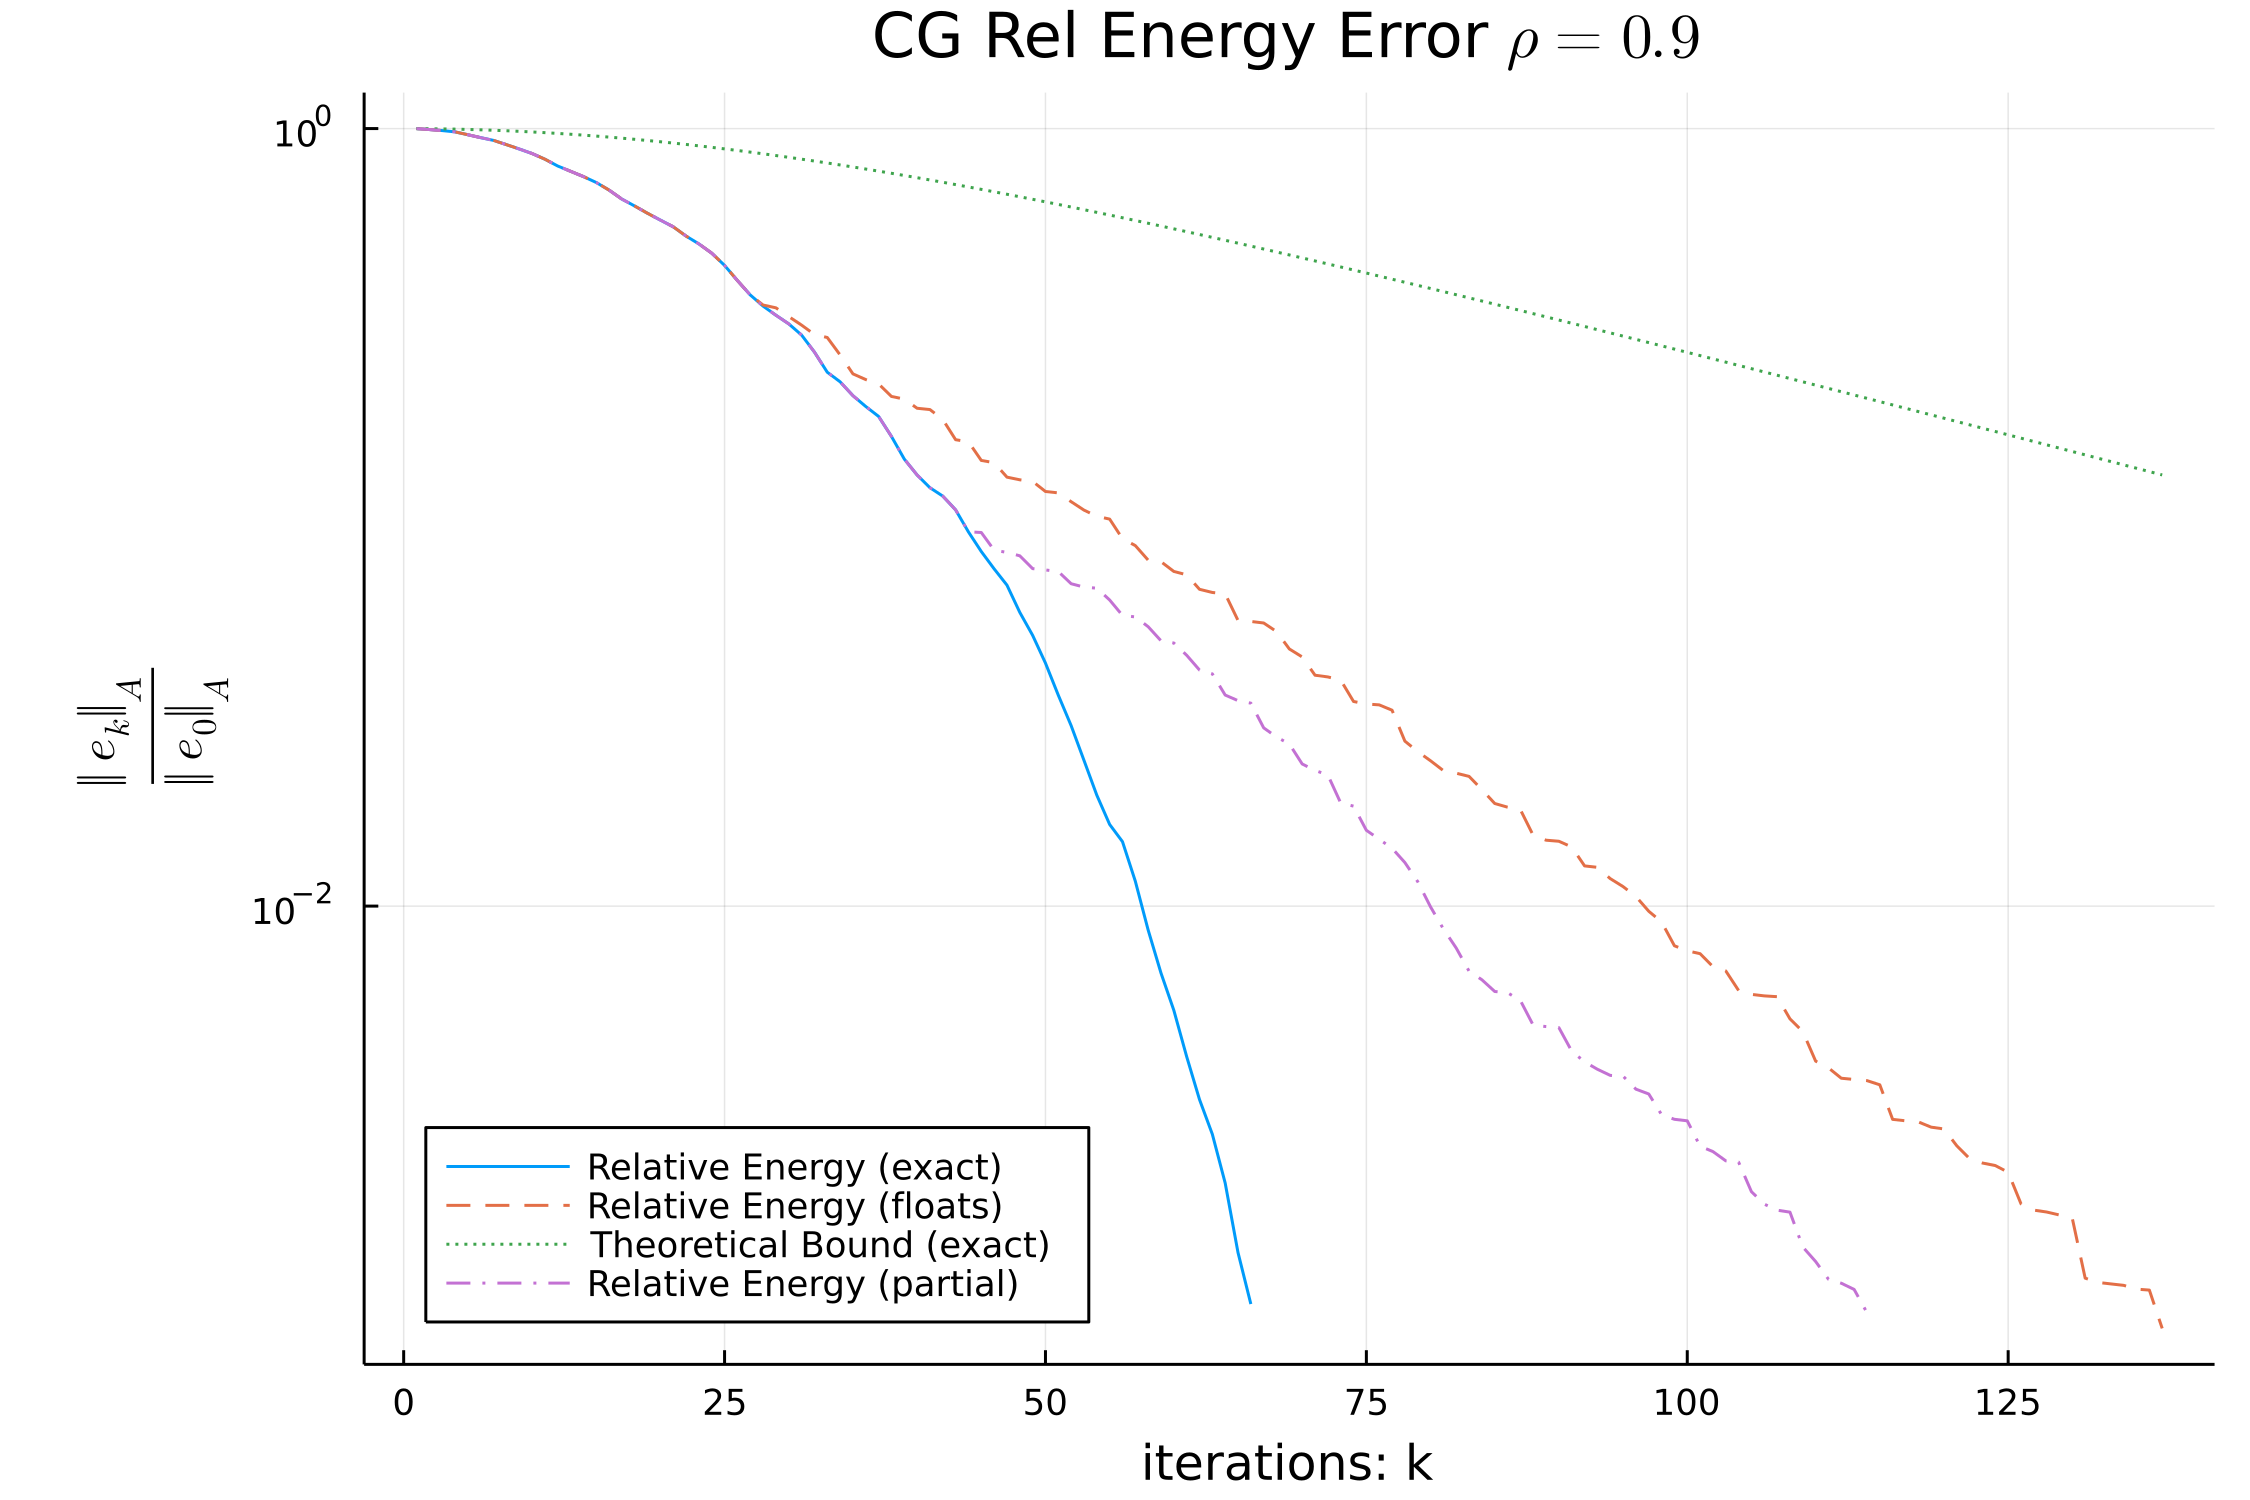
\includegraphics[width=12cm]{cg_convergence_0.9.png}
                    \caption{$\rho = 0.9$}
                    \label{fig:1top}
                \end{subfigure}
                \\[2em]
                \begin{subfigure}[H]{14cm}
                    \centering
                    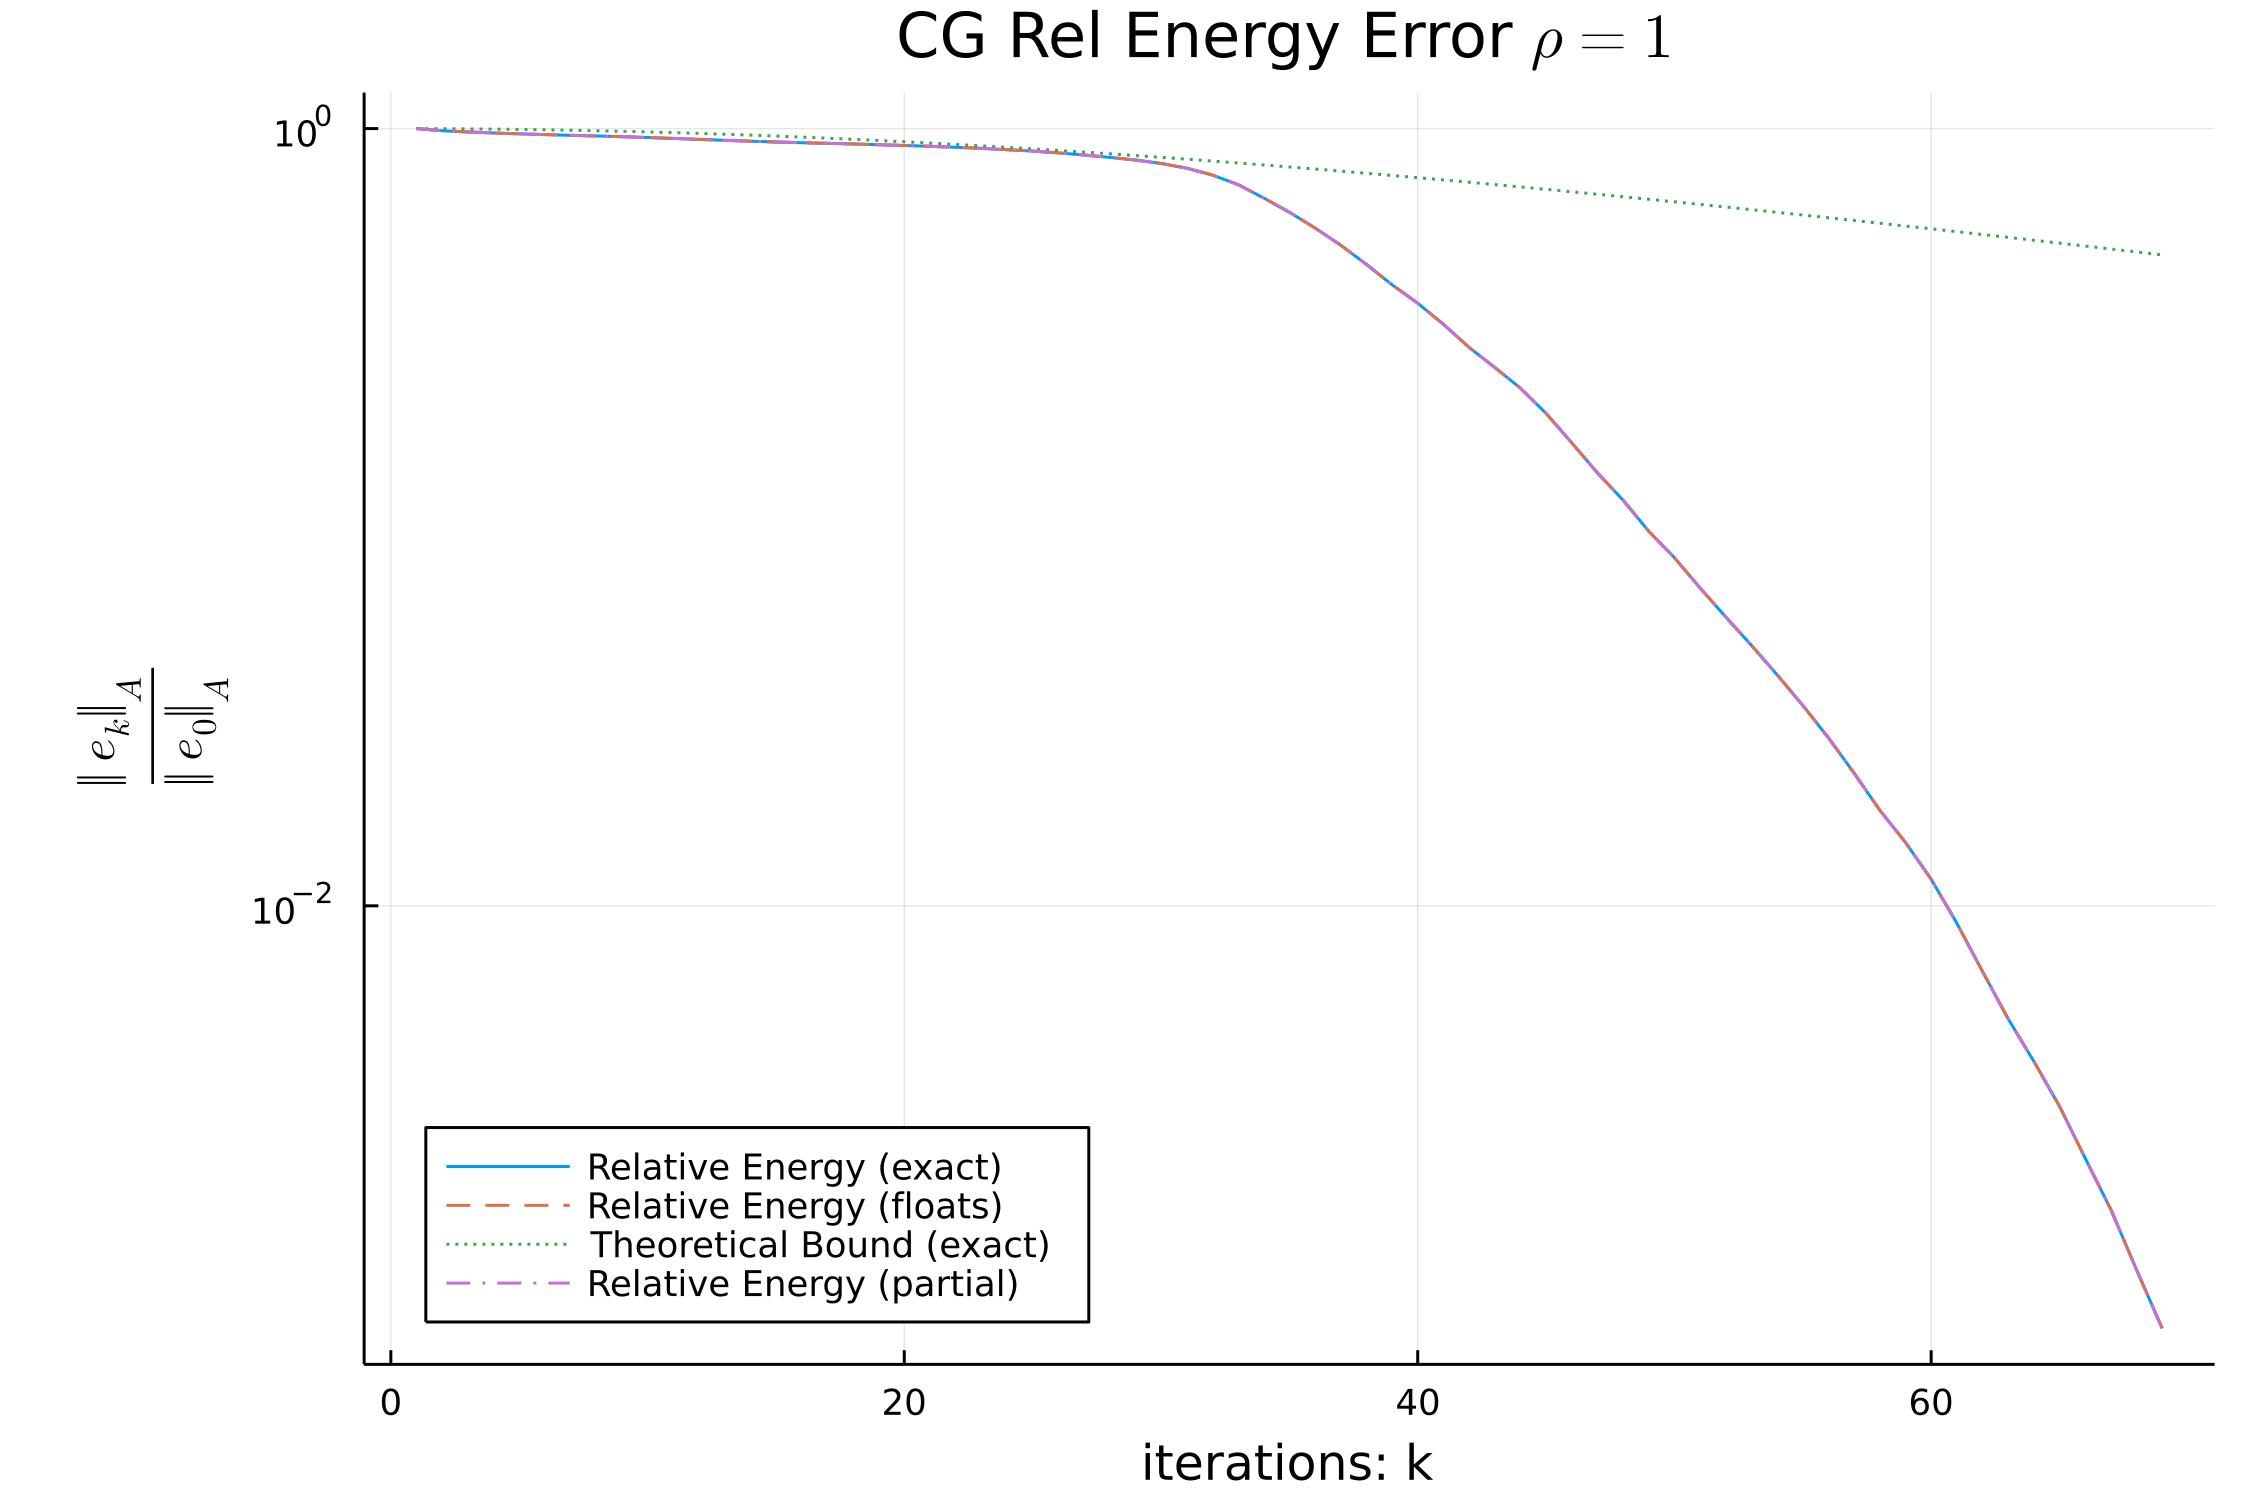
\includegraphics[width=12cm]{cg_convergence_1.png}
                    \caption{$\rho = 1$}
                    \label{fig:1bottom}
                \end{subfigure}
                \caption{
                    The relative energy norm error for different methods. Blue solid line: The exact conjugate gradient convergence. Purple dot dashed: The conjugate gradient that is partially orthogonalized with previous 8 residual and conjugate vectors. orange dashed: the Original conjugate gradient. Green dot: The tighter theoretical upper bound derived by Chebyshev (\hyperref[line:CG_Cheb_Bound]{\ref*{line:CG_Cheb_Bound}}). The matrix is $256\times 256$
                }
                \label{fig:1}
            \end{figure}
            The Chebyshev bound is no longer a tight bound because the distribution of the eigenvalues is not perfectly uniform for $\rho = 0.9$. The partially orthogonalized methods diverge from the exact error after more steps of iterations compared to the relative error without any orthogonalizations. These are seen in \hyperref[fig:1]{(fig \ref*{fig:1top})}. In contrast, on the right with $\rho = 1$, then the eigenvalues are uniformly distributed, the relative energy errors of all 3 methods aligns and overlapped into one curve in \hyperref[fig:1]{(fig \ref*{fig:1bottom})} at the expense of slower convergence for the few iterations at the beginning. 
            \begin{remark}
                The convergence is disappointing under floating-point arithmetic and the promised efficiency of the algorithm is not there anymore even if the matrix is not necessarily ill-conditioned. Just from \hyperref[fig:1]{(fig \ref*{fig:1})} it seems like outlier eigenvalues provide fast convergence under full orthogonalization, but not for floating point. 
                \par
                However, please observe from \hyperref[fig:1]{(fig \ref*{fig:1bottom})} that, all these 3 methods are identical, and the Chebyshev bound is relatively tight at the first few iterations of the algorithm, which is related to the discussion later and linked to the fact that the characteristic polynomial of $T_k$ has roots closer to the spectrum of $A$ where eigenvalues are sparse before converging to region of the spectrum where eigenvalues are denser. 
            \end{remark}
    \subsection{Paige's Convergence rate of CG under Floating Points}
        In this section we present the backwards analysis of the CG convergence rate in a more thorough manner and examine its consequences. When floating-point arithmetic is used, the eigenvalues of the tridiagonal matrices might introduce ghost eigenvectors for the Lanczos Iterations, and using the equivalence of the Lanczos iterations and CG, we can capture a posteriori bound on how much the error is exactly during the iterations of CG. 
        \subsubsection{Bounding the Relative Residuals}
            Recall from proposition \hyperref[prop:Lanczos_Vectors_and_Residuals]{Proposition \ref*{prop:Lanczos_Vectors_and_Residuals}} that the residual of the CG can be expressed in terms of the Lanczos vectors. However, the Lanczos iterations under floating doesn't produces perfectly orthogonal Lanczos Vectors (The lost of orthogonality is experimented and visualized in the next section), $\tilde{Q}_k$ is not quiet orthogonal, which would also means that $\tilde{Q}_k^HA\tilde{Q}_k\approx T_k$ where $T_k$ is the results from the Lanczos iterations will not equal to $\tilde{Q}^T_kA\tilde{Q}_k$. However the Lanczos iterations will still solve for $y_k$ using the expression $y_k = \beta T^{-1}_k\xi_1$, the algorithm still thought $T_k$ produced by itself is perfectly tridiagonal. As a result, the algorithm never quite finds the optimal under the conjugate basis. At first glance, tiny round-off errors in the Lanczos vectors are very problematic. 
            \par
            Surprisingly, the recurrence formula for Lanczos still holds to some extent, in addition we can leverage the fact that $y_k$ is solved exactly and assume: $y_k = \beta T^{-1}\xi_1$ is at least, exact. Then it left us with fewer types of floating-point errors to keep track of. Next, we proceed to look for the residual of the CG algorithm by stating that the Lanczos recurrences\footnote{statement 2.11 from C. C. Paige's 1980 paper.\cite{paper:paige1980}. The result is surprising in the sense that $Q_k$ being none orthogonal in finite precision won't affect the recurrence.}: 
            \begin{align}
                AQ_k = Q_{k + 1} \begin{bmatrix}
                    T_k
                    \\
                    \beta_k \xi_k^T
                \end{bmatrix} + F_k
            \end{align}
            Reader, please reflect on the fact that the $Q_k$ which is not orthogonal, and we are fixing the recurrences with $F_k$, a matrix representing the floating error to correct it so that the equality holds true. $\Vert F_k\Vert$ is small and it's on the magnitude of $\mathcal O(\epsilon \Vert A \Vert)$. 
            \begin{align}
                r_k &= r_0 - AQ_ky_k
                \\
                r_k &= r_0 - 
                    \left(
                        Q_{k + 1} \begin{bmatrix}
                            T_k
                            \\
                            \beta_k \xi_k^T
                        \end{bmatrix}
                        + 
                        F_k
                    \right)
                y_k
                \\
                r_k &= 
                \underbrace{\left(
                    r_0 - Q_{k + 1}\begin{bmatrix}
                        T_k
                        \\
                        \beta_k \xi_k^T
                    \end{bmatrix}y_k
                \right)}_{= -\beta_k\xi_k^Ty_kq_{k + 1}} + F_k \beta T_k^{-1}\xi_1
                \\
                \implies
                \frac{\Vert r_{k + 1}\Vert}
                {
                    \Vert r_0\Vert
                } &\le
                \beta_k \Vert
                    \xi_k^T T_k^{-1}\xi_1 q_{k + 1}
                \Vert + 
                \Vert F_kT_k^{-1}\xi_1 \Vert
                \\
                \frac{\Vert r_{k + 1}\Vert}
                {
                    \Vert r_0\Vert
                } 
                &\le 
                \beta_k |
                    \xi_k^T T_k^{-1}\xi_1
                | + 
                \Vert F_k\Vert  \Vert T_k^{-1}\xi_1\Vert
            \end{align}
            We make use of \hyperref[prop:Lanczos_Vectors_and_Residuals]{Proposition \ref*{prop:Lanczos_Vectors_and_Residuals}} and obtain a similar expression because it didn't make use of the fact that $Q_k$ is orthogonal. This time, we take $F_k$ into account. The residual is now bounded by the sum of scalar $\xi_k^T T_k^{-1}\xi_1$ and the floating-point error matrix $F_k$ produced by the Lanczos iterations. 
            \begin{remark}[When Finite Arithmetic Lanczos is Exact]\label{remark:CG_Float_Remark}
                We can bound the first term that made up the upper bound for the residual of CG using previous convergence results of CG under exact arithmetic; recall \hyperref[theorem:CG_Convergence_Rate]{CG convergence rate (theorem \ref*{theorem:CG_Convergence_Rate})}. It can be applied here for the first term in (5.3.6): 
                $\beta_k |
                \xi_k^T T_k^{-1}\xi_1|$. 
                \par
                This is true because if we were to perform an CG on the $T_{k + 1}$ produced by the finite precision algorithm with the initial Lanczos vector $q_1$ being $\xi_1^{(n)}$, then its residual $\overline{r}_{k}$ of equivalent CG would be exact and it's given as $-\beta_kT_{k}^{-1}\xi_kq_{k + 1}$, but with $q_{k + 1} = \xi_{k + 1}^{(n)}$, the $k + 1$ th standard basis vector in $\mathbb R^{n}$, and $T_k = (T_{k + 1})_{1:k, 1:k}$. And to our excitement, we already have the bound for $\overline{r}_{k+1}$ proven in \hyperref[theorem:CG_Convergence_Rate]{theorem \ref*{theorem:CG_Convergence_Rate}}.
            \end{remark}

        \subsubsection{Paige's Theorem and Floating-point Convergence of CG}
            We now introduce a new theorem proposed by Paige in chapter 4 of Greenbaum's book\cite{book:greenbaum}, originally appeard in 3.48 of C.C Paige's Thesis(\cite{paper:paige1980}). It gives a bound to the floating-point errors for the CG by bounding the condition number of $T_k$ from Lanczos iterations. It's stated as follows: 
            \begin{theorem}[Paige's Theorem]\label{theorem:paige1}
                The eigenvalues $\theta_i^{(j)}, i = 1, \cdots, j$ of the tridiagonal matrix $T_j$ satisfies: 
                \begin{align}
                    & 
                    \lambda_1 - j^{5/2}\epsilon_2\Vert A\Vert 
                    \le \theta_i^{(j)}
                    \le 
                    \lambda_n + j^{5/2}\epsilon_2\Vert A\Vert
                    \\
                    &
                    \epsilon_2 := \sqrt{2}\max\{6\epsilon_0, \epsilon_1\}
                \end{align}
            \end{theorem}
            Along with this theorem, the following quantities from Paige are also defined and cited in Greenbaum book chapter 4. 
            \begin{align}
                & \epsilon_0 \equiv 2(n + 4)\epsilon
                \\
                & \epsilon_1 \equiv 2(7 + m \Vert  \;|A|\;\Vert/\Vert A\Vert)\epsilon
                \\
                & \epsilon_0 < \frac{1}{12} \quad k(3\epsilon_0 + \epsilon_1) < 1
                \\
                & \Vert F_k\Vert \le \sqrt{k}(\epsilon_1) \Vert A\Vert
                \\
                & \Vert q^T_jq_j -1\Vert \le 2\epsilon_0
                \\
                & \beta_j \le \Vert A\Vert(1 + (2n + 6)\epsilon + j(3\epsilon_0 + \epsilon_1))
            \end{align}
            The quantity $k$ is the current iterations number of the Lanczos Iterations, $j\le k$. $m$ is the maximum number of non-zero elements in the matrix $A$. 
            Using Paige's theorem, we can bound the condition number for the matrix $T_{k + 1}$ produced by the finite precision Lanczos, which is given by: 
            \begin{align}
                \tilde{\kappa} = \frac{\lambda_n + (k + 1)^{5/2}\epsilon_2\Vert A\Vert}
                {\lambda_1 - (k + 1)^{5/2} \epsilon_2\Vert A\Vert}
            \end{align}
            Using \hyperref[remark:CG_Float_Remark]{(remark \ref*{remark:CG_Float_Remark})}, we can make the following proposition
            \begin{prop}
                \begin{align}
                    | \beta_k\xi_k^TT_k^{-1}\xi_1 | \le 
                    2 \sqrt{\tilde{\kappa}}\left(
                        \frac{\sqrt{\tilde{\kappa}} - 1}{\sqrt{\tilde{\kappa}} + 1}
                    \right)^k
                \end{align}    
                Where $\tilde\kappa$ is the bound of the condition number of the $T_k$ matrix (from (5.3.15)), the tridiagonal matrix produced by the finite precision Lanczos. 
            \end{prop}
            \begin{proof}
                Using the \hyperref[lemma:Relative_Energy_Norm_and_Relative_2_Norm_Conversions]{lemma \ref*{lemma:Relative_Energy_Norm_and_Relative_2_Norm_Conversions} in appendix}, we can derive the relations between the 2-norm of the relative residuals and the energy norm of the relative error: 
                \begin{align}
                    \frac{\Vert Ae_k\Vert}{\Vert Ae_0\Vert}
                    & \le 
                    \kappa(T_k)\frac{\Vert e_k\Vert_A}{\Vert e_0\Vert_A}
                    \le 2\sqrt{\kappa(T_k)}
                    \left(
                        \frac{\sqrt{\tilde{\kappa}} - 1}{\sqrt{\tilde{\kappa}} + 1}
                    \right)^k
                    \\
                    \frac{\Vert r_k\Vert}{\Vert r_0\Vert} &= 
                    | \beta_k\xi_k^TT_k^{-1}\xi_1 | \quad \text{by \hyperref[remark:CG_Float_Remark]{(remark \ref*{remark:CG_Float_Remark})}}
                    \\
                    \implies | \beta_k\xi_k^TT_k^{-1}\xi_1 | 
                    &\le 
                    2 \sqrt{\tilde{\kappa}}
                    \left(
                        \frac{\sqrt{\tilde{\kappa}} - 1}{\sqrt{\tilde{\kappa}} + 1}
                    \right)^k
                \end{align}
                The third inequality is simply from \hyperref[theorem:CG_Convergence_Rate]{CG Convergence Rate (theorem \ref*{theorem:CG_Convergence_Rate})} when we assume that the eigenvalues are uniformly distributed convex hull of the spectrum of $A$. The first fraction is actually the relative error of the 2-norm of the residual because $Ae_k = r_k$ by definition. Substituting the quantity $\kappa(T_k)$, the condition number of the matrix $T_k$, which we figured out using Paige's theorem and denoted it as $\tilde{\kappa}$. 
            \end{proof}
            Finally, if we assume that $T_k^{-1}$ is actually invertible, which requires that the conditions for all the quantities: $\epsilon_0, \epsilon_1$ holds true, and $\lambda_1 - (k + 1)^{5/2} \epsilon_2\Vert A\Vert > 0$. Finally, we make can bound the relative residual of the CG algorithm by considering: 
            \begin{align}
                \frac{\Vert r_{k + 1}\Vert}
                {
                    \Vert r_0\Vert
                } &\le
                \beta_k \Vert
                    \xi_k^T T_k^{-1}\xi_1 q_{k + 1}
                \Vert + 
                \Vert F_kT_k^{-1}\xi_1 \Vert
                \\
                & \le 
                \beta_k|\xi_k^T T_k^{-1}\xi_1|
                \Vert q_{k + 1}\Vert + 
                \Vert F_k\Vert  \Vert T^{-1}_k\xi_1\Vert
                \\
                & \le 
                2 \Vert q_{k + 1}\Vert\sqrt{\tilde{\kappa}}
                    \left(
                        \frac{\sqrt{\tilde{\kappa}} - 1}{\sqrt{\tilde{\kappa}} + 1}
                    \right)^k
                + 
                \sqrt{k}(\epsilon_1) \Vert A\Vert 
                \Vert T^{-1}_k\Vert
            \end{align}
            Now, observe that $|q_j^Tq_j - 1|\le 2\epsilon_0$ from (5.3.13), which implies that $\Vert q_{k + 2}\Vert^2 \le (1 + 3\epsilon_0)$ which is $\Vert q_{k + 1}\Vert \le \sqrt{1 + 2\epsilon_0}$. In pursuit of mathematical beauty, we look for alternative expression for the quantity $\Vert A\Vert \Vert T^{-1}_k\Vert$ giving us: 
            \begin{align}
                \Vert A\Vert\Vert T_k^{-1}\Vert &= \frac{\lambda_n}{\lambda_1 - k^{5/2}\epsilon_2\Vert A\Vert} \le \tilde{\kappa}
                \\
                \implies 
                \frac{\Vert r_{k + 1}\Vert}
                {
                    \Vert r_0\Vert
                } &\le 
                2  \sqrt{1 + 2\epsilon_0}\sqrt{\tilde{\kappa}}
                    \left(
                        \frac{\sqrt{\tilde{\kappa}} - 1}{\sqrt{\tilde{\kappa}} + 1}
                    \right)^k
                + \sqrt{k}(\epsilon_1) \tilde{\kappa}
            \end{align}
            Which completes the proof for the upper bound on the convergence rate for the Conjugate Gradient Method under floating-point arithmetic. 
            \begin{remark}
                This proof showed that the $T_{k + 1}$ generated by floating point CG is nonsingular, $\beta_k \neq 0$, the restrictions for the quantities of \hyperref[theorem:paige1]{theorem \ref*{theorem:paige1}} then the CG method will continue to converge in the future iterations. So in layman's terms, it doesn't matter if the round-off error accumulated, Conjugate Gradient will converge as long as the problem is not too insane, or $A$ being too pathological to deal with. 
                \par
                Finally, I want to point out the fact that Paige's theorem (\hyperref[theorem:paige1]{theorem \ref*{theorem:paige1}}) is derived using forward error analysis on the Lanczos Iterations, which is the absolute worst case. For most cases in modern computing platforms, the summation process of vector dot products has much higher floating-accuracy compare to older computing platforms due to the use of parallelism, or floating-point specific summation instructions, which reduces the relative sizes for the summands, hence reducing the total round-off error accumulations. The bound of convergence rate we derive can be a huge over estimation. 
            \end{remark}

    \subsection{Ghost Eigenvalues and Losing Orthogonality}
        The name ghost eigenvalues refers to the phenomena where the Lanczos Algorithm seems to produce tridiagonal matrix $T_k$ whose eigenvalues are clustered extremely close to a simple eigenvalues of the matrix $A$, when in fact, those extremely close eigenvalues are a single eigenvalue of the original matrix $A$'s spectrum. 
        \par
        The name ``ghost eigenvalues'' was spotted from lecture 36 of Trefethen's Book\cite{book:trefethen}, the exact origin of the term is not important. This phenomena is more pronounce to eigenvalues in the exterior of $A$'s spectrum. We know for a fact that the tridiagonal matrix produced via Lanczos can't have any repeated eigenvalues (\hyperref[prop:Irreducible Symmetric Tridiagonal Matrix]{appendix item \ref*{prop:Irreducible Symmetric Tridiagonal Matrix}}). What happens in this case is the floating point error propagating through the Lanczos Iterations causing lost of orthogonality of $Q_k$ and eventually produce ghost eigenvalues. 
        \subsubsection{Ghost Eigenvalues Experiments}
            Here, we conducted numerical experiments and carefully reproduce the phenomena for a diagonal matrix $A$ with diagonals given by the formula: 
            \begin{align}
                \lambda_i = \left(-1 + \frac{2(i - 1)}{(n - 1)}\right)^3 \quad 1\le i \le n
            \end{align}\label{eqn:the_ill_conditioned_matrix}
            where $A\in \mathbb R^{n\times n}$. This matrix is particularly good for reproducing the phenomena. For this experiment, we set $n = 64$ and we use Float64. 
            \par
            We run the Lanczos iterations with $q_1$ being the vector of all ones, we marked the smallest and largest 10 eigenvalues during the iterations and plotted their trajectories from iteration 20 to 64. The results can be seen in \hyperref[fig:2]{(figure \ref*{fig:2} left)}. On \hyperref[fig:2]{figure \ref*{fig:2} right}, we made the plot for what would happen if the Lanczos iterations are free of numerical round-off error. We didn't use exact arithmetic, instead, we simply re-orthogonalized all the Lanczos vector $q_k$ using all previously obtained Lanczos vectors to emulate the effect, which is just an Arnoldi iteration. Please bear in mind that there are eigenvalues in the middle interior part of the spectrum, they are just not plotted in the figure. 
            \begin{figure}[H]
                \centering
                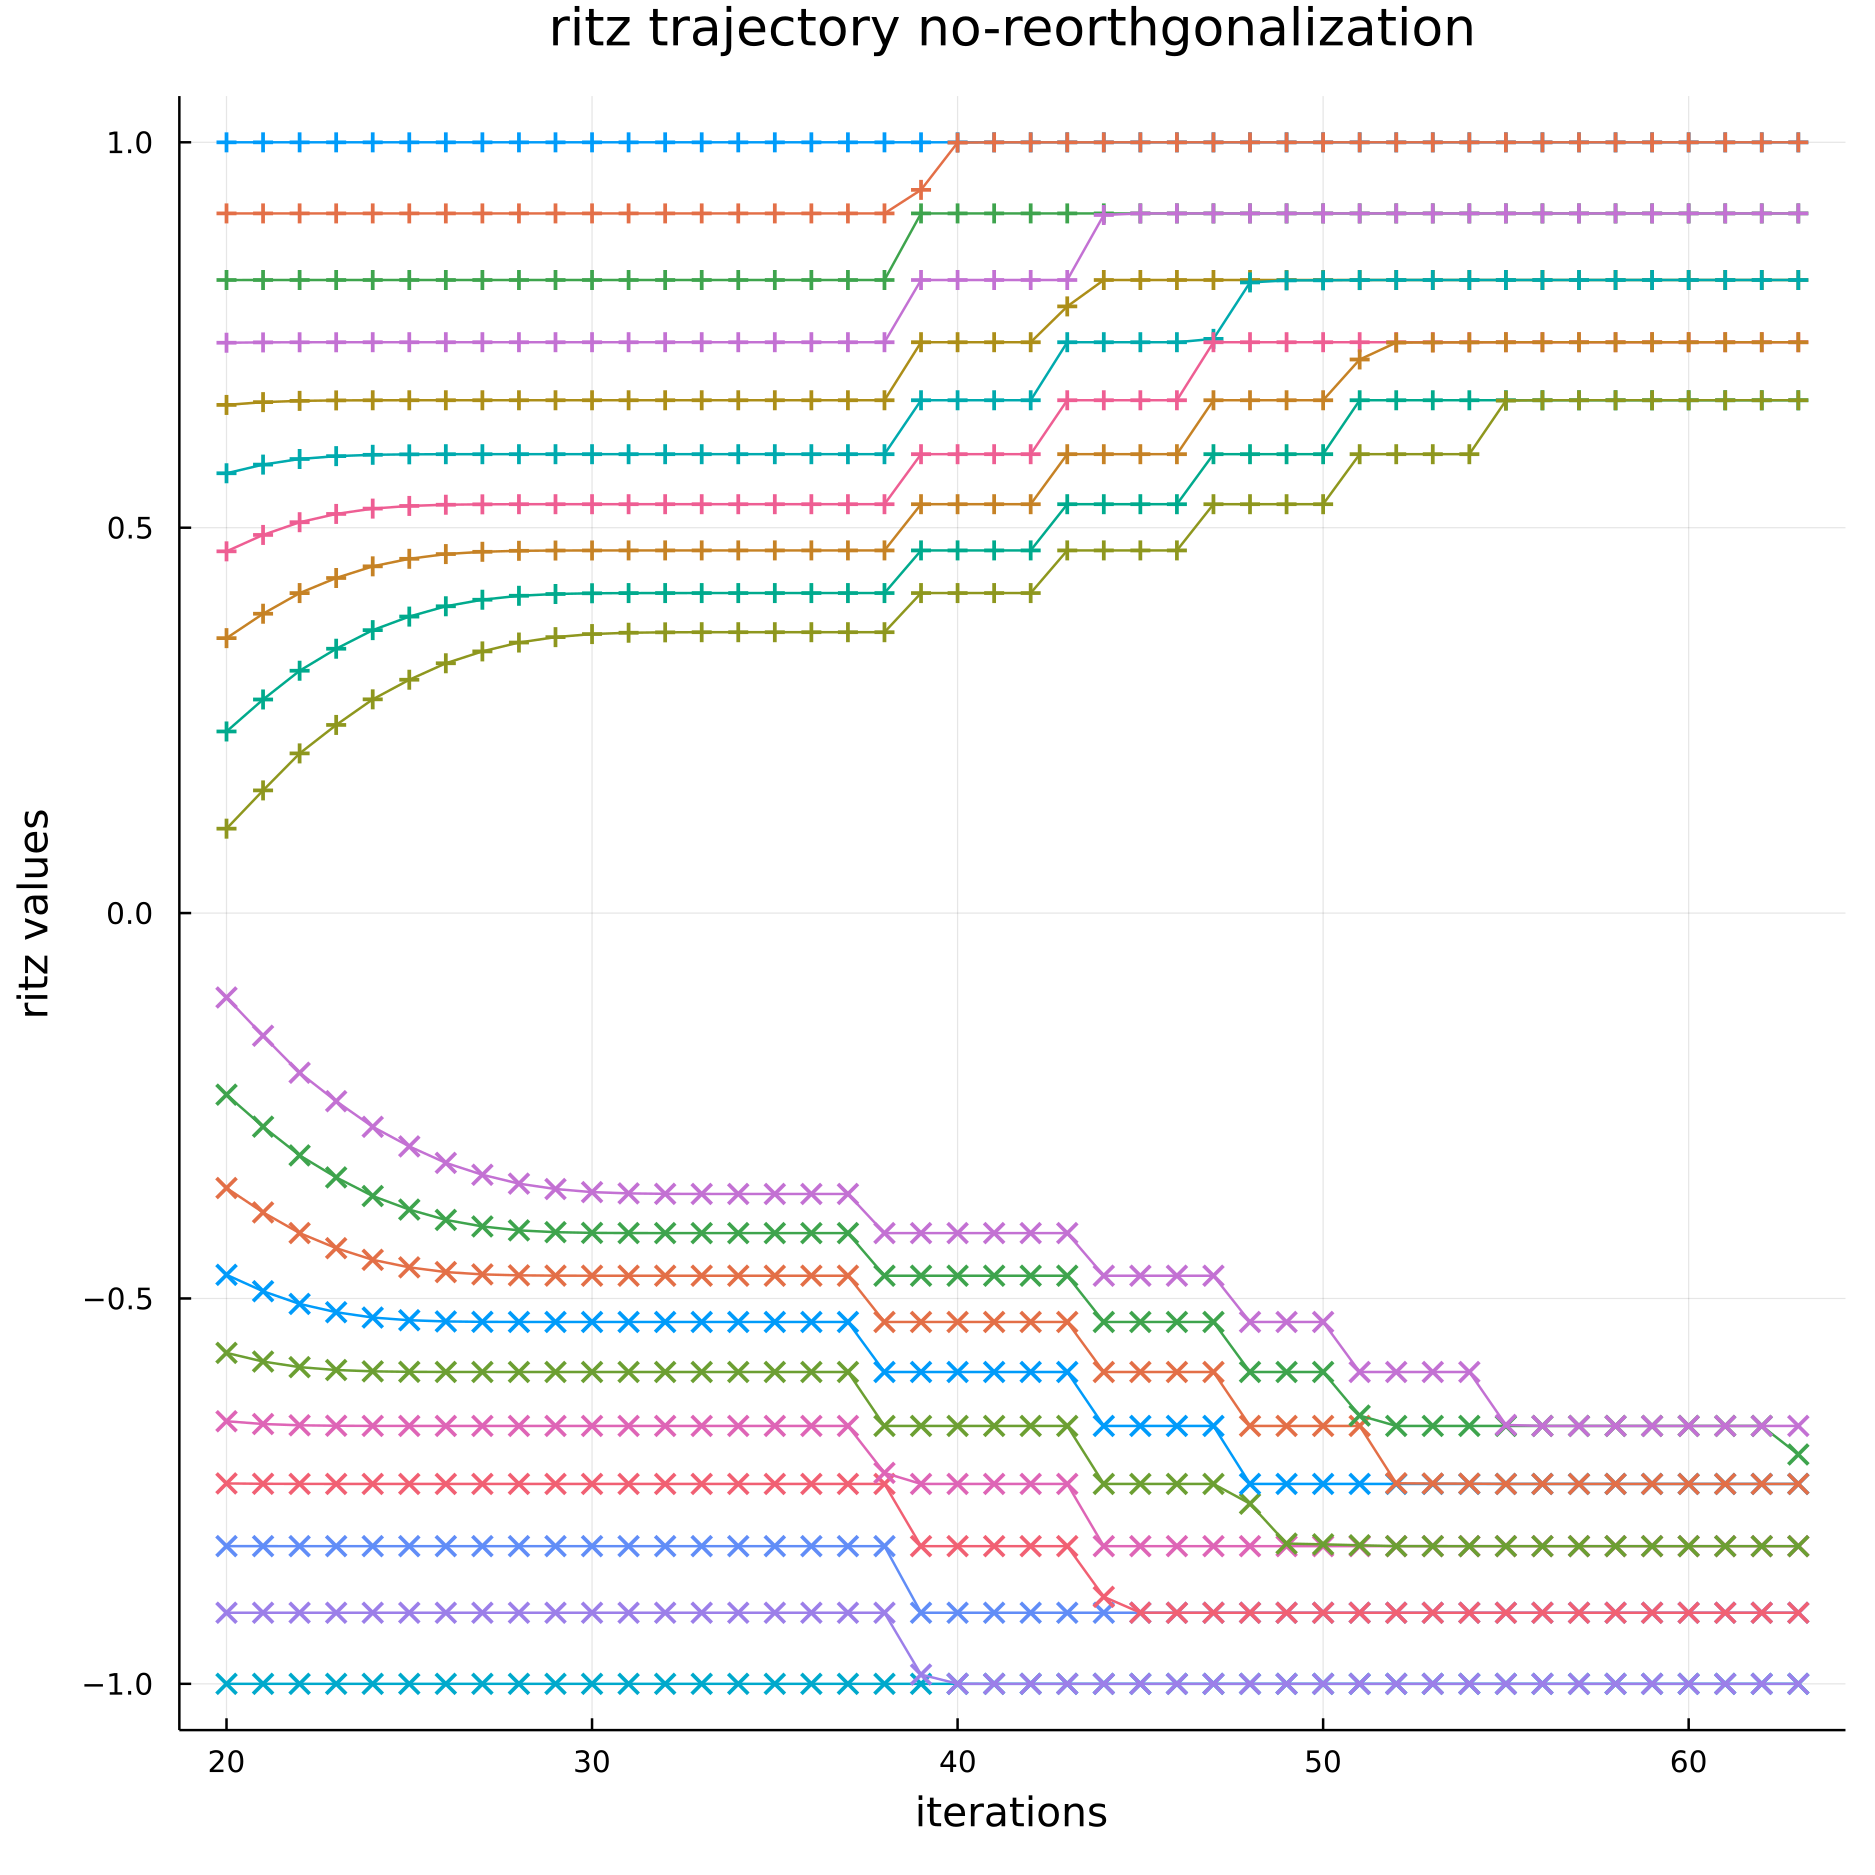
\includegraphics[width=8cm]{ritz_trajectory_plot_floats.png}
                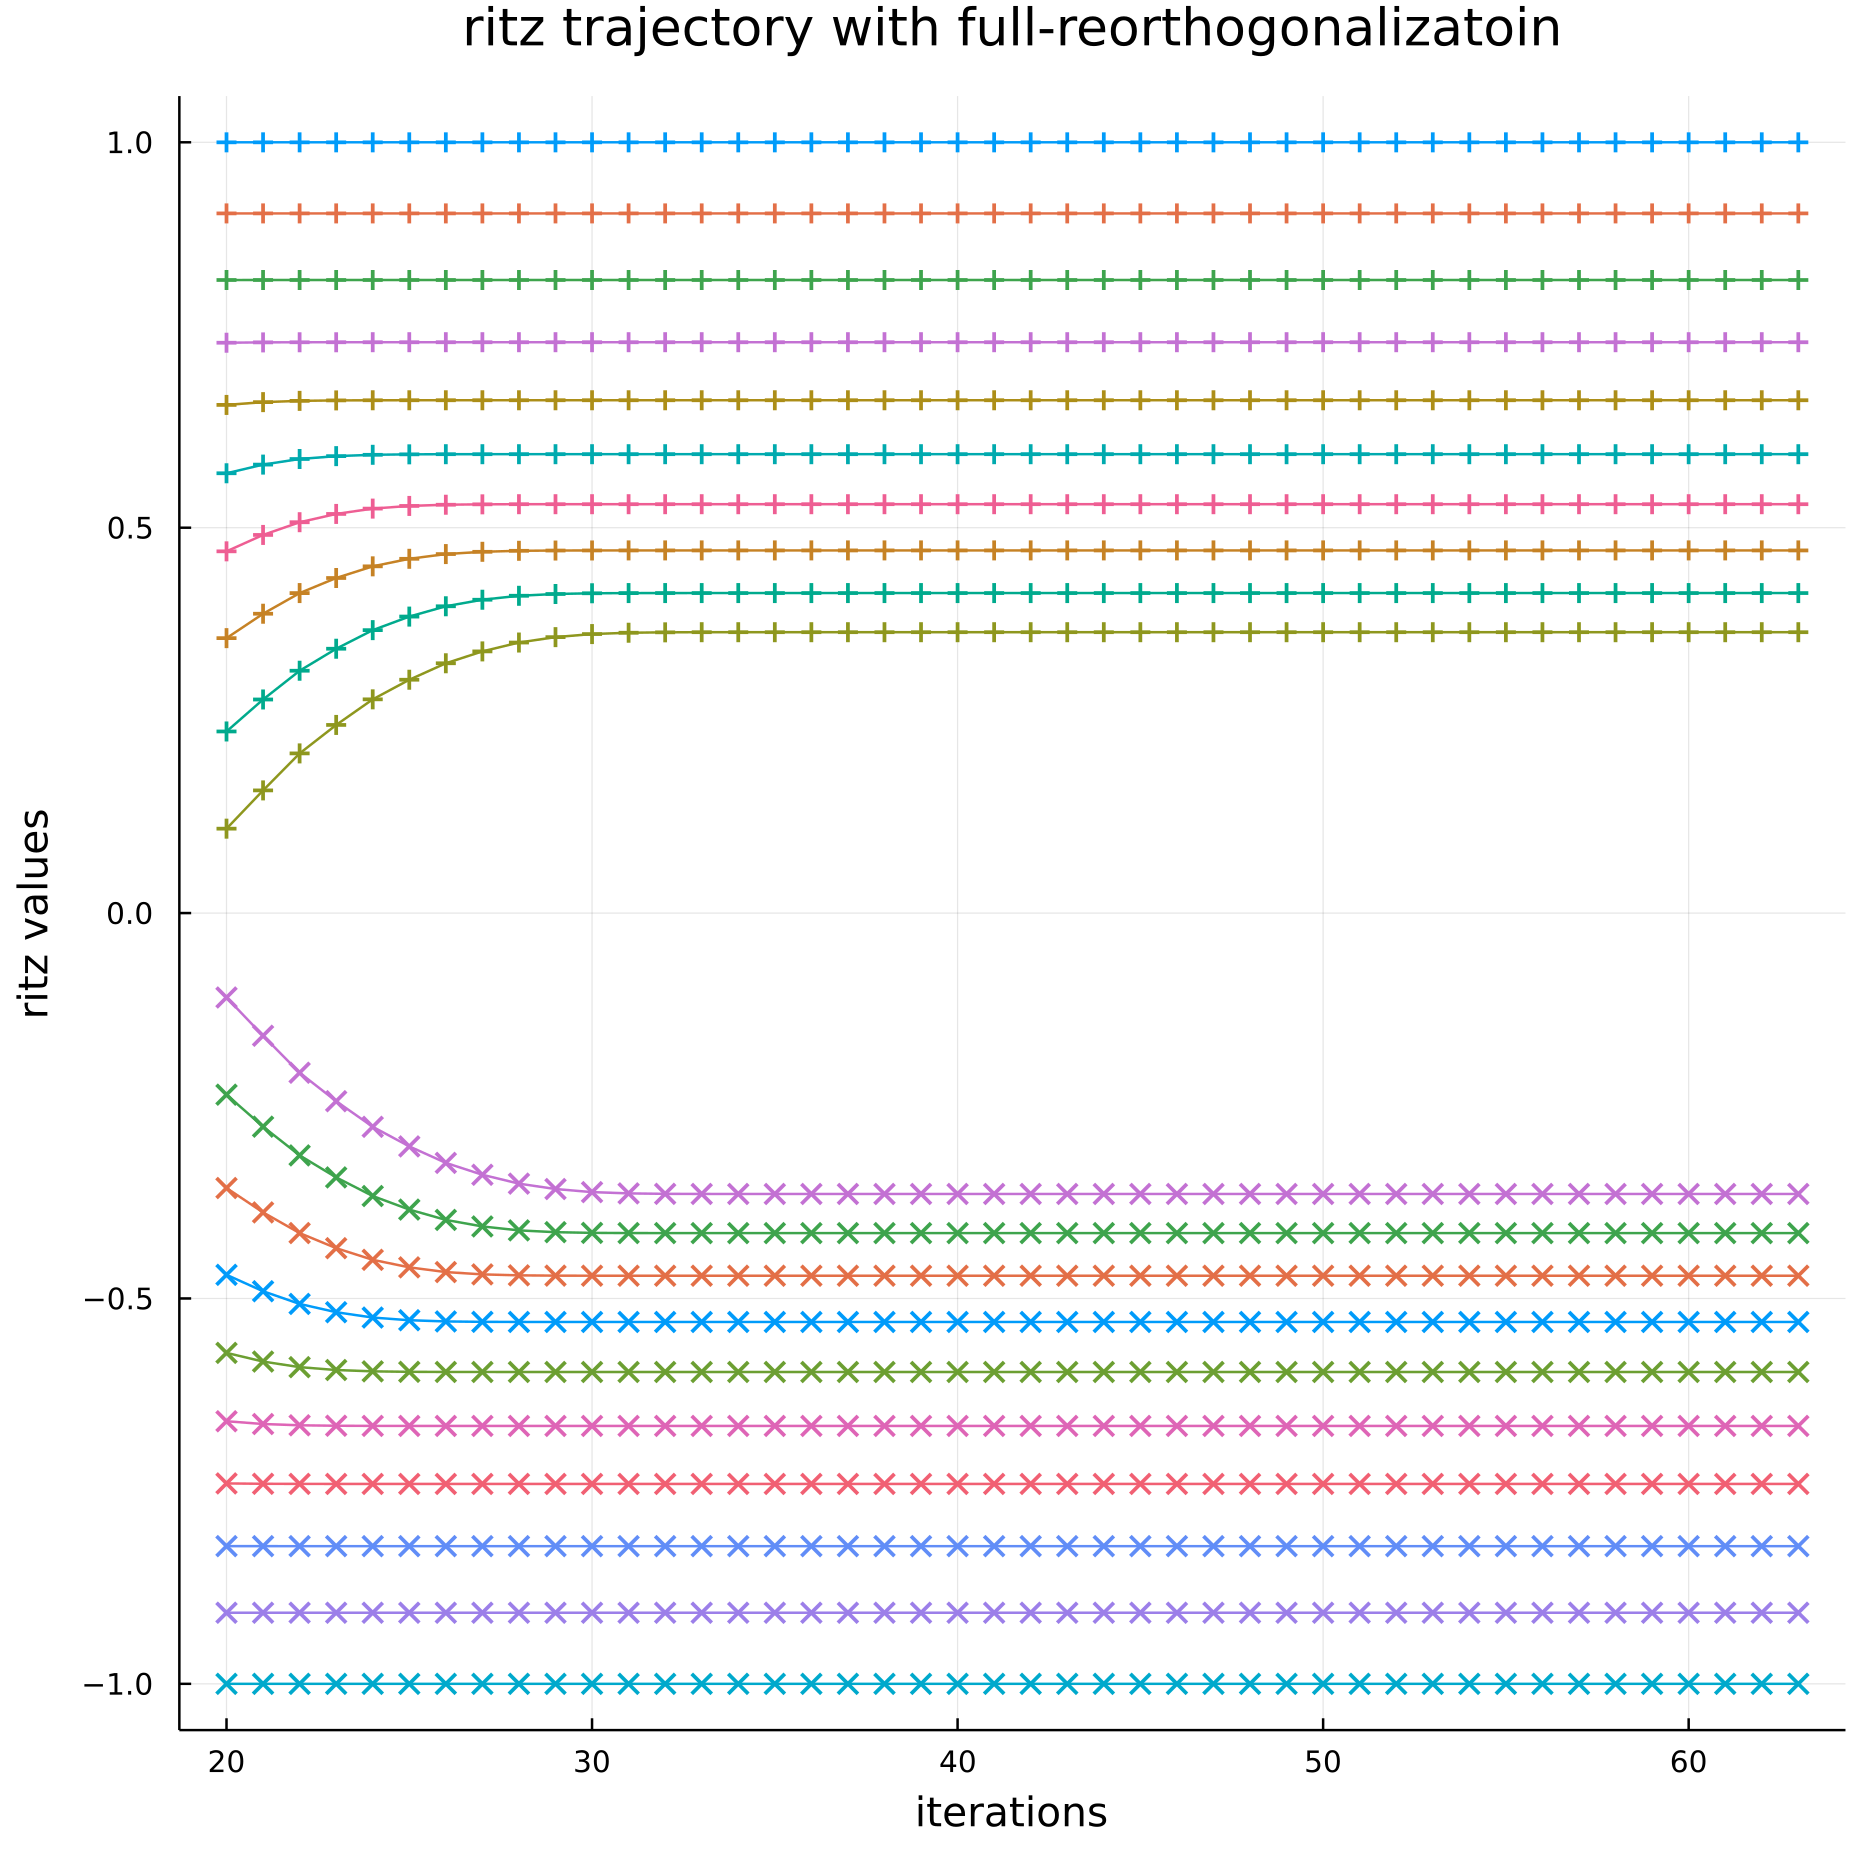
\includegraphics[width=8cm]{ritz_trajectory_plot_exact.png}
                \caption{The highest and lowest 10 eigenvalues of the matrix $T_k$ during the Lanczos Iterations are being tracked by their relative order. During each iteration, the first, the second, the third, ... etc eigenvalues of $T_k$ are linked together by a line in a different color. Left is Lanczos with numerical round-off error, right is Lanczos iterations that fully re-orthogonalize $q_k$ for each iteration which emulates the behaviors under exact arithmetic. }
            \end{figure}\label{fig:2}
            Recall from the \hyperref[theorem:cauchy_interlace]{Cauchy Interlace Theorem (theorem \ref*{theorem:cauchy_interlace})}, the eigenvalues of the tridiagonal matrix $T_{k + 1}$ has to be in between each eigenvalues of $T_{k}$ except for the first and the last eigenvalue of $T_{k + 1}$.  This implies that, the $\theta_i^{(k)}$, the $i$ th eigenvalues during the $k$ th iteration will move monotonically upwards or downwards during the Lanczos iterations. The ghost eigenvalues on the figure appear when some of the interior eigenvalues suddenly switch to another eigenvalue's trajectory that is on the exterior of the spectrum. It appears as though the matrix $T_k$ has repeated eigenvalues which we know is not true due to (\hyperref[prop:Irreducible Symmetric Tridiagonal Matrix]{appendix item \ref*{prop:Irreducible Symmetric Tridiagonal Matrix}}), they are just very close. 
            \par
            However, judging the eigenvalues of the matrix $T_k$ alone WILL NOT distinguish between two very close eigenvalues correspond to two different eigenvalues of $A$ or it's due to the floating-point round-off error. It also will NOT tell whether the Lanczos vectors are losing orthogonality, even if the eigenvalue trajectories seem to suggest it. The lost of orthogonality must happen for the Lanczos vector while at the same time, we observed extremely close eigenvalues of $T_k$ clustring around eigenvalues of $A$ to confirm the fact that they are indeed ghost eigenvalues. 
            \par
            We can't tell it because if I keep the matrix $T_k$ we used to  produce \hyperref[fig:2]{fig \ref*{fig:2}} generated from a Lanczos iterations and use it as $A$ with $q_1 - \xi_1$, then it will reproduce exactly the same graph as in left of \hyperref[fig:2]{fig \ref*{fig:2}} when we plot out the trajectories of the eigenvalues of $T_k$, but the $Q_k$ in this case is the $k\times k$ identity matrix and it's exact (Using the exact same idea appeared in \hyperref[remark:CG_Float_Remark]{remark \ref*{remark:CG_Float_Remark}}). Now consider performing another Lanczos iterations $A:=T_k$ it but with the initial vector $\xi_1$, then we will exactly reproduce $A$ itself because it's tridiagonal. But in this case, the eigenvalues of $T_k$ are exact after termination of Lanczos iteration. In this case, all eigenvalues are actually presented in the original matrix $A$, which is just $T_k$, itself. 
            \par
            In fact, the ghost eigenvalues here are produced by floating-point errors because firstly we know what the actual eigenvalues of $A$ is, we made $A$. To make sense of it better intuitively, we observe from the experiments that the loss of orthogonality of $Q_k$ happens together with ghost eigenvalues on the spectrum of $T_k$. If the $Q_k$ matrix is perfectly orthogonal, then there are no ghost eigenvalues, regardless of what the trajectories of the eigenvalues of $T_k$ look like. In fact, a corresponding plot of $Q_k^HQ_k$ are plotted in \hyperref[fig:3]{(fig \ref*{fig:3} left)} for demonstrating the loss of orthogonality for the same diagonal matrix $A$ proposed earlier. We plotted the heat map of the matrix $Q^H_kQ_k$ directly as well.
            \begin{figure}[H]
                \centering
                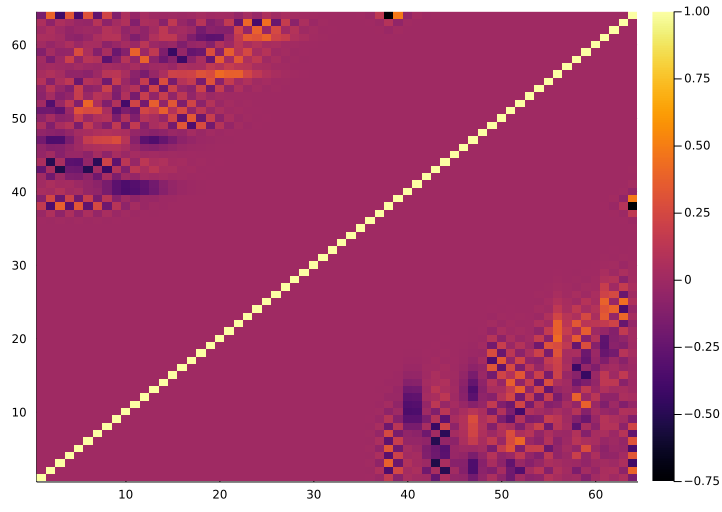
\includegraphics[width=8cm]{fig3.png}
                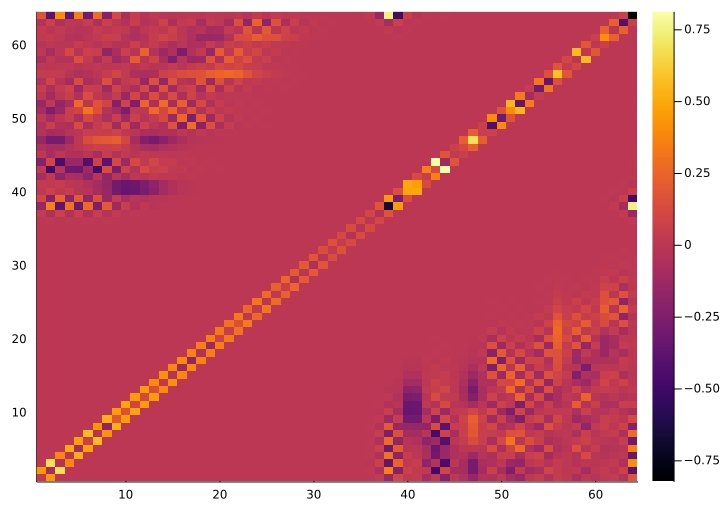
\includegraphics[width=8cm]{fig4.png}
                \caption{left: The heatmap of the plot of the absolute values of the matrix $Q^T_kQ_k$. right: The plot of $Q_k^TAQ_k$ from floating-point Lanczos iterations}
            \end{figure}\label{fig:3}
            In addition to the lost orthogonality of the matrix $Q_k$, we also visualized the actual tridiagonal matrix reproduced by $Q_kAQ_k$ which is plotted in \hyperref[fig:3]{(fig \ref*{fig:3} right)}. Observe that most of the off tridiagonal entries are non-zero and relatively huge, which doesn't worry us too much because $A$ itself has a large condition number. What is concerning is the blob of non-zero entries on the top left and the bottom right of the plot. And this is a significant loss of orthogonality created by floating point arithmetic. 
            \begin{remark}
                As a final remark for these numerical experiments, I suggest an intuitive way of understanding them. Which will be useful when we actually wish to analyze it rigorously. Simply put, the Lanczos Iterations might ``forget'' about the eigenvalues when it converged (usually manifested as the stable trajectories of eigenvalues on the exterior of the spectrum for the matrix $T_k$ in \hyperref[fig:2]{(fig \ref*{fig:2})}), and when it happens, the Lanczos vectors produced by the algorithm has lost its orthogonality correspondingly, which then causes the interior eigenvalues of $T_k$ to shift, creating ghost eigenvalues that doesn't exist in the spectrum of $A$. 
                \par
                Secondly, there is another phenomenon of Ritz values during the iterations of Lanczos iterations called misconvergence. It describes the process which a Ritz value is stuck between two eigenvalues of $A$, stagnated for few iterations and then suddenly shifts away, which is extremely similar to the shifting we observed in \hyperref[fig:2]{figure \ref*{fig:2}}. It happens when 2 eigenvalues of matrix $A$ is extremely close to each other. It should not be confused with ghost eigenvalues because they are two distinct phenomena where misconvergence can happen under exact arithmetic. For more description of such phenomena, refer to the book by M. G. Cox and S. Hammarling \cite{book:reliable_computation}. 
            \end{remark}
        \subsubsection{Lanczos Vectors Losing Orthogonality on converged Ritz vectors}
            To gain a better understanding, let's define the notion of Ritz values and Ritz vectors. For our discussion, the Ritz value $\theta_i^{(k)}$ are the $i$ th eigenvalues of the matrix $T_k$ from the and the Ritz vectors are $Q_ks_{i}^{(k)}$ where $s_i^{(k)}$ is the $i$ th eigenvector for the matrix $T_k$. Recall from \hyperref[remark:Minimal_Polynomial_from_Lanczos_Iterations]{remark 3.4.2}, the characteristic polynomial of $T_k$ is the monic polynomial that minimizes the 2-norm error for the vector $p_k(A)q_1$ among all monic of the same degree; therefore intuitively, the Ritz values and Ritz vectors approximates eigenvalues and eigenvectors of matrix $A$ due to the apprixmating characteristic polynomial. Let's suppose that $s_i^{(k)}$ for $T_k$ is a good approximation for $\lambda_j$, let's consider the Lanczos iterations recurrences: 
            \begin{align}
                AQ_k &= Q_k T_k + q_{k + 1}\beta_k\xi_k^T
                \\
                AQ_ks_i^{(k)} &= \theta_j^{(k)} Q_k s_i^{(k)} + q_{k + 1}\beta_k \xi_k^Tv
                \\
                AQ_ks_i^{(k)} &= \theta_j^{(k)} Q_k s_i^{(k)} + \beta_kq_{k + 1}(s_i^{(k)})_k
                \\
                AQ_ks_i^{(k)} - \theta_j^{(k)} Q_k s_i^{(k)} &=   \beta_kq_{k + 1}(s_i^{(k)})_k
            \end{align}
            Upon brief examinations, convergence of the Ritz value $\theta_{i}^{(k)}$ depends on $\beta_k$ and $(s_i^{(k)})_k$, intuitively as the Krylov subspace expands, it contains more and more space for the the eigenvectors of $A$, and the Ritz vector will have more ``room'' to get closer to the eigenvector of $A$, by the approximation property of Lanczos. Assuming good convergence of $s_i^{(k)}$ convergences so that the value of $\beta_k, (s_i^{(k)})_k$ are both small (it's true regardless of orthogonality of $Q_k$), then we consider the projection of most recent lanczos vector $q_k$ onto the Ritz vector $Q_ks_i^{(k)}$, which is $q_k^TQ_ks_i^{(k)} = (s_i^{(k)})_k$. We expect the projection onto the Ritz vector to be small if the Ritz vector is converging to an eigenvector of $A$.  
            \par
            However, under floating-point arithmetic, once the Ritz vector $s_i^{(k)}$ is converging to an eigebvalue of $A$, then the projection of the latest Lanczos vector onto the Ritz vector begins to grow. On the plot showed in \hyperref[fig:4]{figure \ref*{fig:4}}, we projected the log absolute value of $q_k^TQ_ks_i^{(k)}$ for $i=1, 2, 3$ for all $k=20, \cdots, 64$, and we used the same setup from the last section where we demonstrated ghost eigenvalues. For comparison, \hyperref[fig:5]{figure \ref*{fig:5}} showed us what happens in exact arithmetic. One very important observation to make from \hyperref[fig:5]{figure \ref*{fig:5}} is that the peak of the blue curve, projection onto the largest Ritz value happens around iteration 3.8, and around that exact same iteration in \hyperref[fig:2]{figure \ref*{fig:2}} is when the second-largest eigenvalue of $T_k$ decides to shift over to the blue curve. Bear in mind that this is in a log plot, and without the log it looks like a sharp spike. 
            \par
            While floating arithematic may sometimes cause the most recent Lanczos vector to lose orthogoality against converged Ritz vectors, the converse is not true. The phenomena itself doesn't imply the fact that floating point error is present and it's causing lost of orthogonality of Lanczos iterations, much similar to what had been discussed about ghost eigenvalues. To illustrate, an experiment is conducted in this way: 
            \begin{enumerate}
                \item [1.] $T_n$ is generated from the diagonal matrix $A$ from finite precision Lanczos iterations. The same setup from \hyperref[eqn:the_ill_conditioned_matrix]{ghost eigenvalues \ref*{eqn:the_ill_conditioned_matrix}}. 
                \item [2.] Lanczos is then performed on $T_k$ initalized with $q_1 = \xi_i$. 
                \item [3.] The projection the most recent lanczos vector $q_k$ is projected onto $Q_ks_i^{(k)}$ for $1\le i \le 3$. Notice that $Q_k$ is gonna be the $k\times k$ identity matrix. `'
            \end{enumerate}
            The results of the projection are showed in \hyperref[fig:6]{fig \ref*{fig:6}}. Please observe that prjection onto the second Ritz vector $Q_ks_2^{(k)}$ seems to decrease and them jumped up again. This happens around the same iterations when the second largest eigenvalue of $T_k$ shift to the trajectory of the largest eigenvalue in \hyperref[fig:2]{fig \ref*{fig:2} left}. However, this time the matrix $Q_k$ is perfect orthogonal. Therefore, small ritz projections of the most recent Lanczos vector doesn't mean that the Ritz value has converged for all future iterations. If $q_k$ is losing orthgonality against some Ritz vectors after it has converged, it doesn't mean that $Q_k$ is losing orthogonality. 
            \begin{figure}[H]
                \centering
                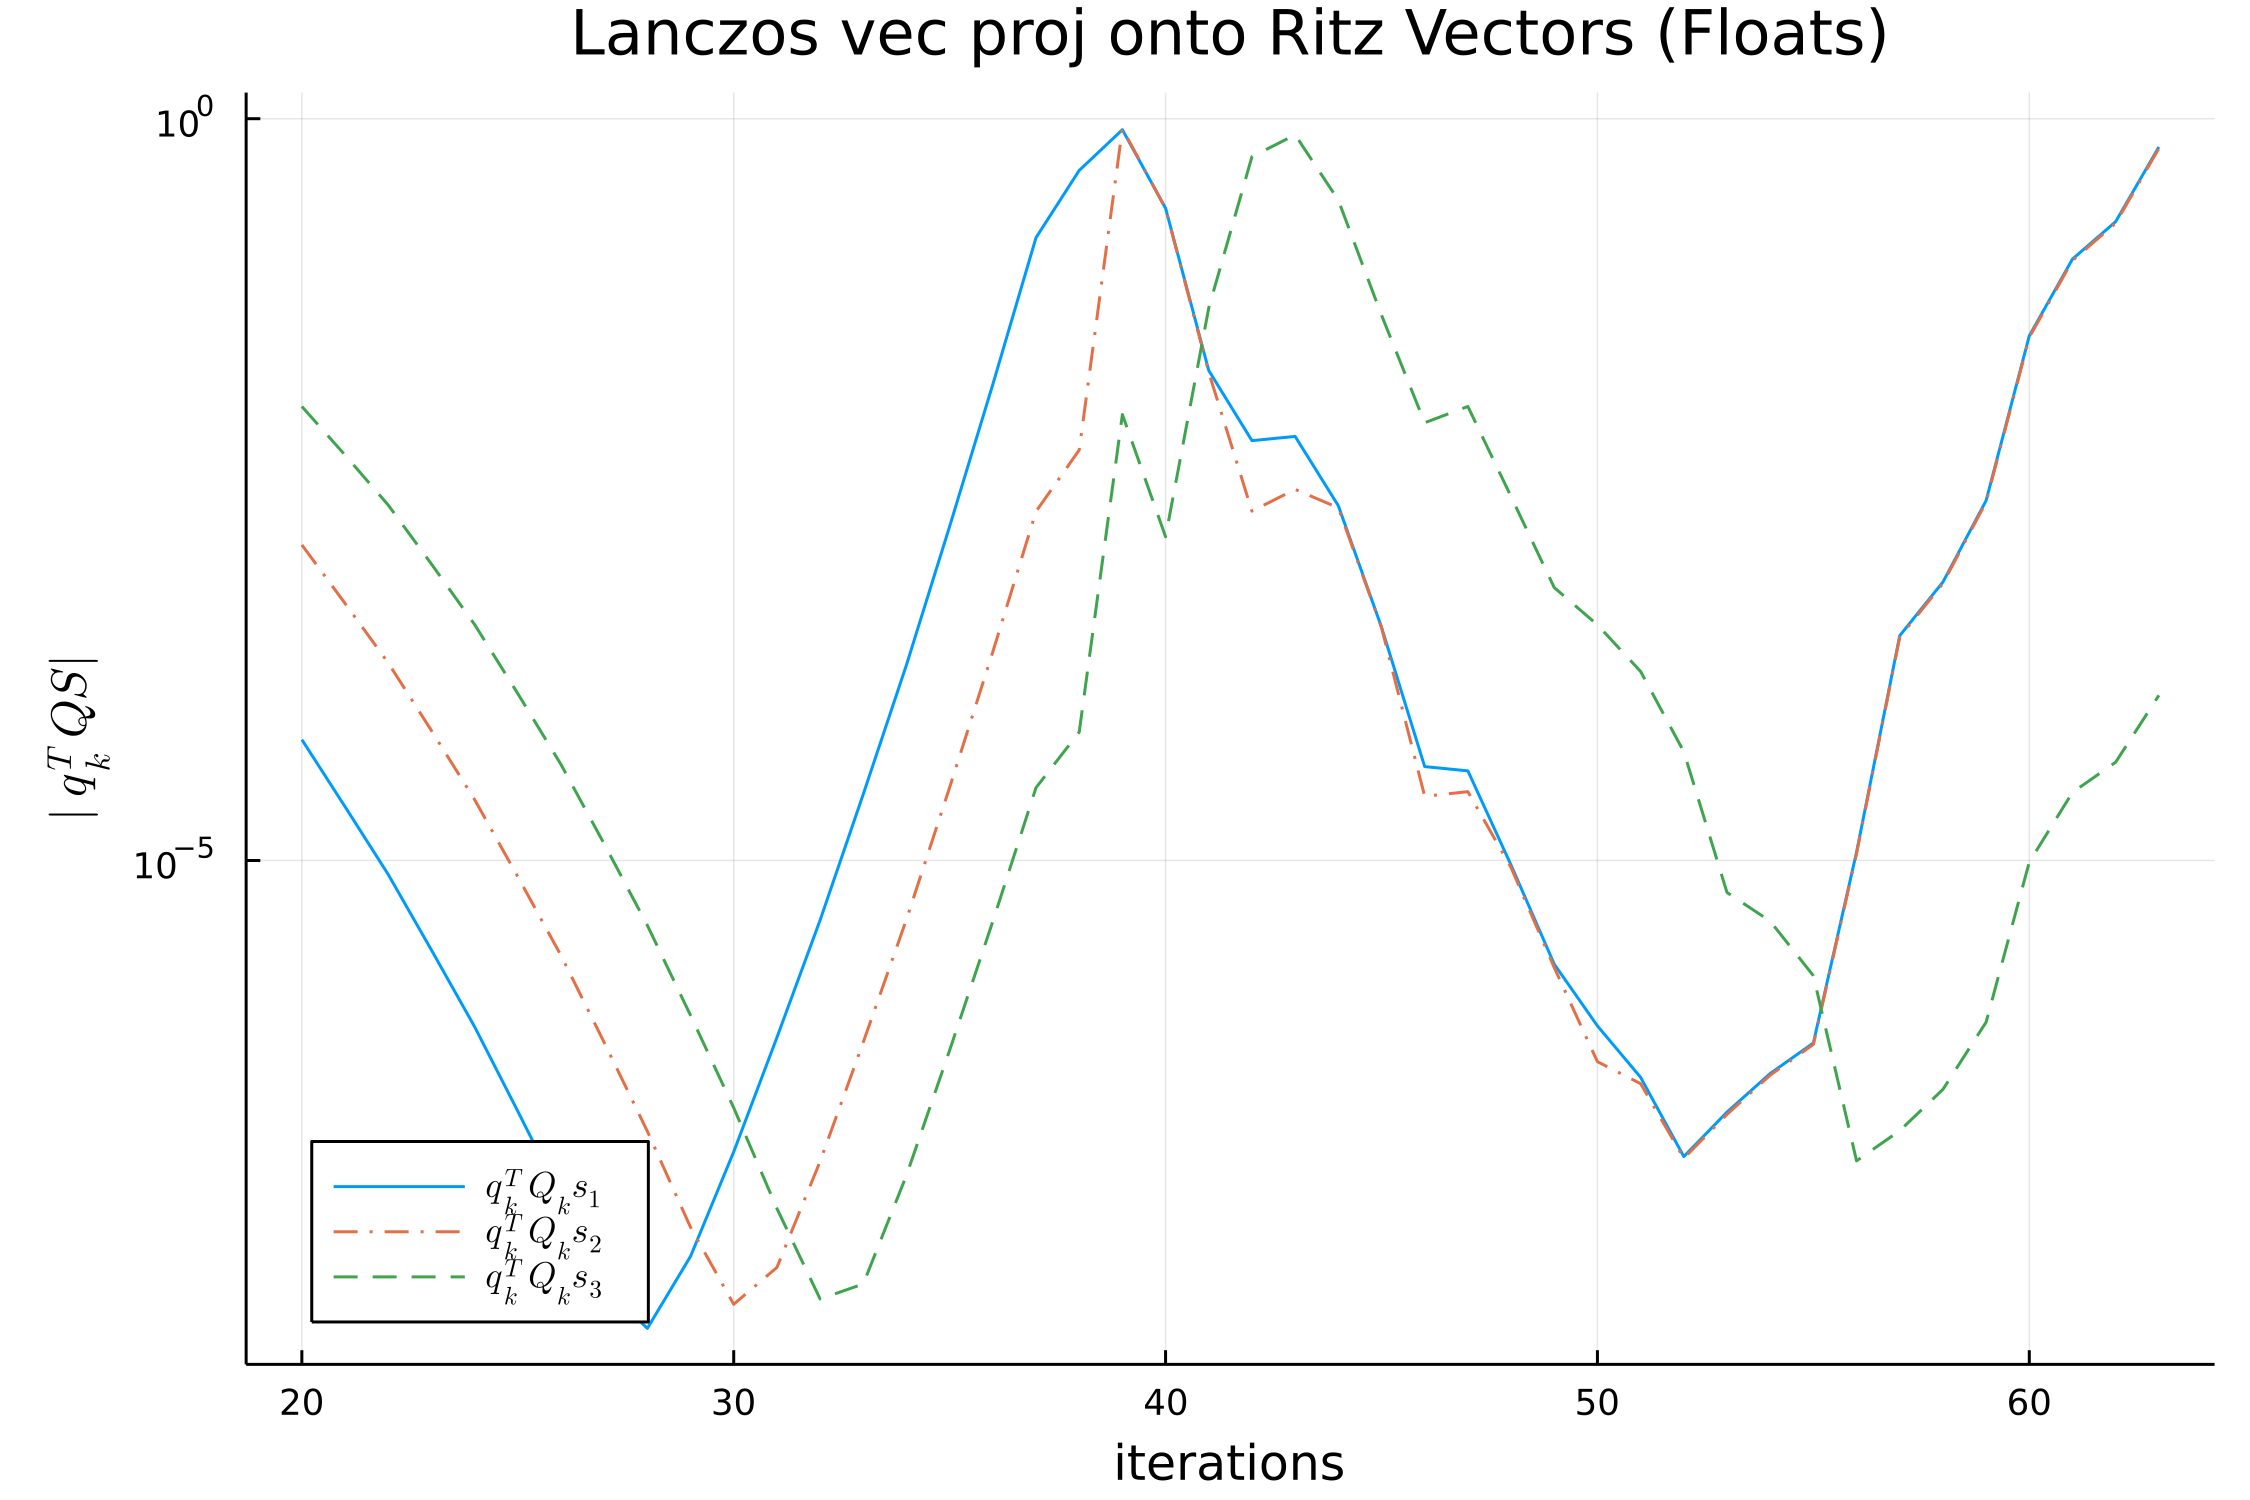
\includegraphics[width=14cm]{lanczos_proj_on_ritz_float.png}
                \caption{Projection of floating-point Lanczos vector $q_k$ onto 3 of the largest Ritz vectors: $Q_ks_i^{(k)}$, for $i = k, k - 1, k - 2$
                }
            \end{figure}\label{fig:4}
            \begin{figure}[H]
                \centering
                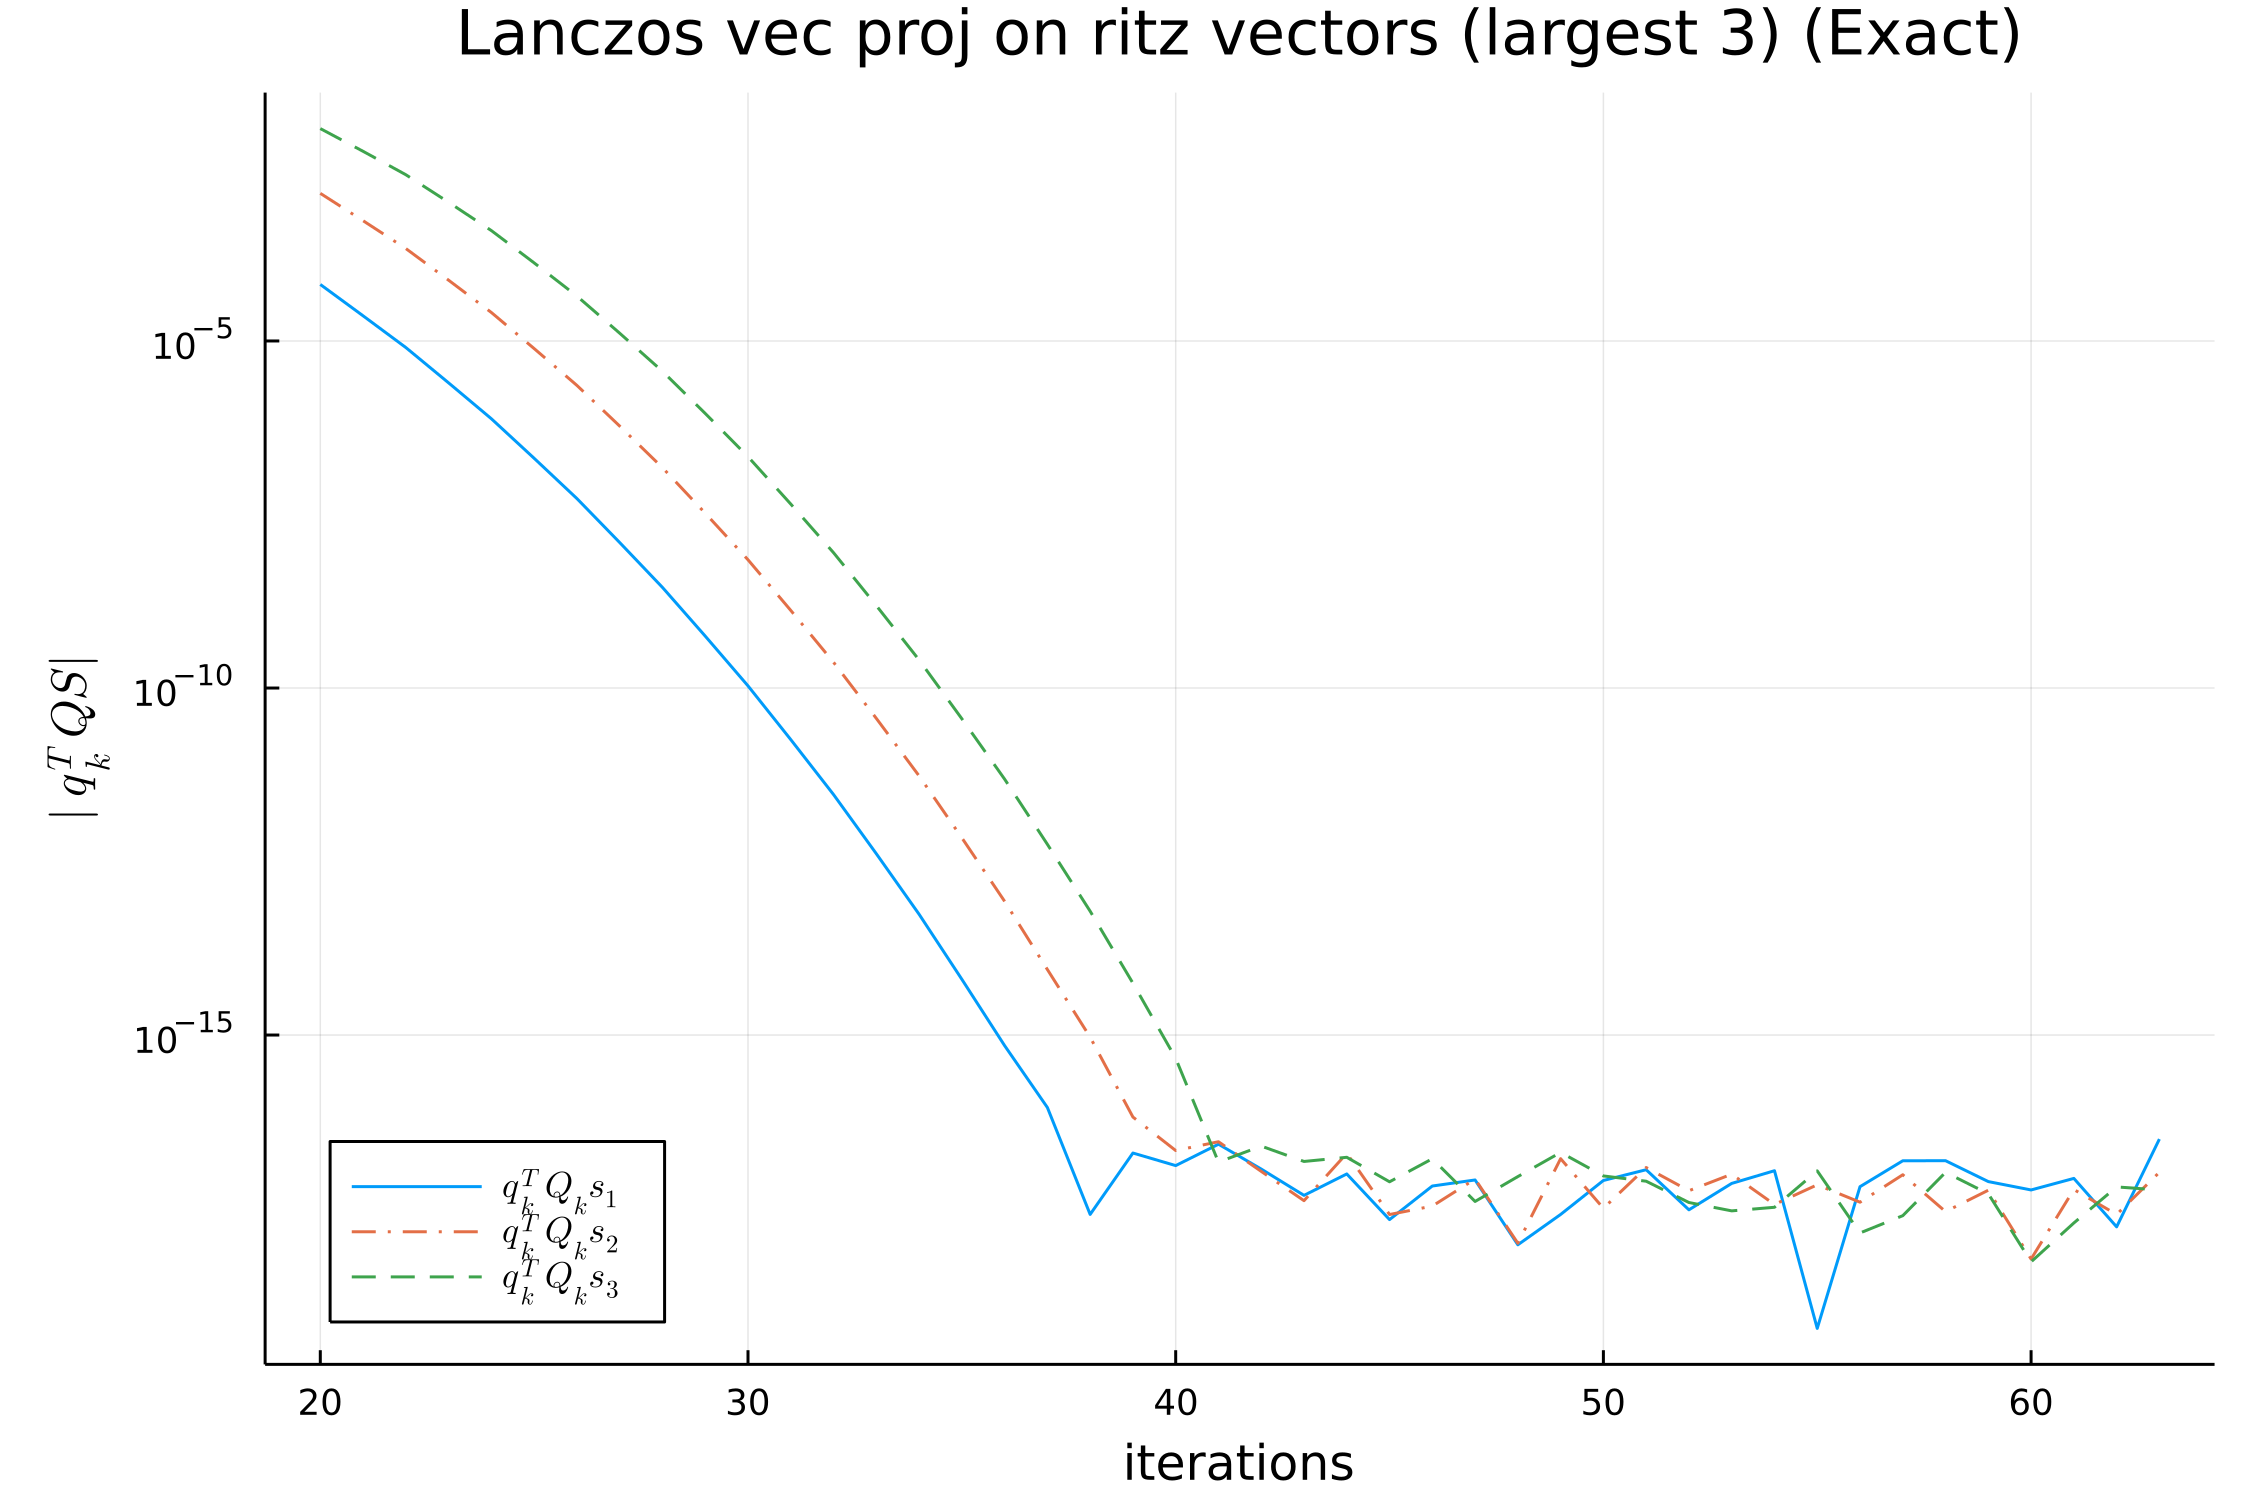
\includegraphics[width=14cm]{lanczos_proj_on_ritz_exact.png}
                \caption{prHjection of the exact Lanczos vector $q_k$ onto 3 of the largest Ritz vectors: $Q_ks_i^{(k)}$, for $i = k, k - 1, k - 2$}
            \end{figure}\label{fig:5}
            \begin{figure}[H]
                \centering 
                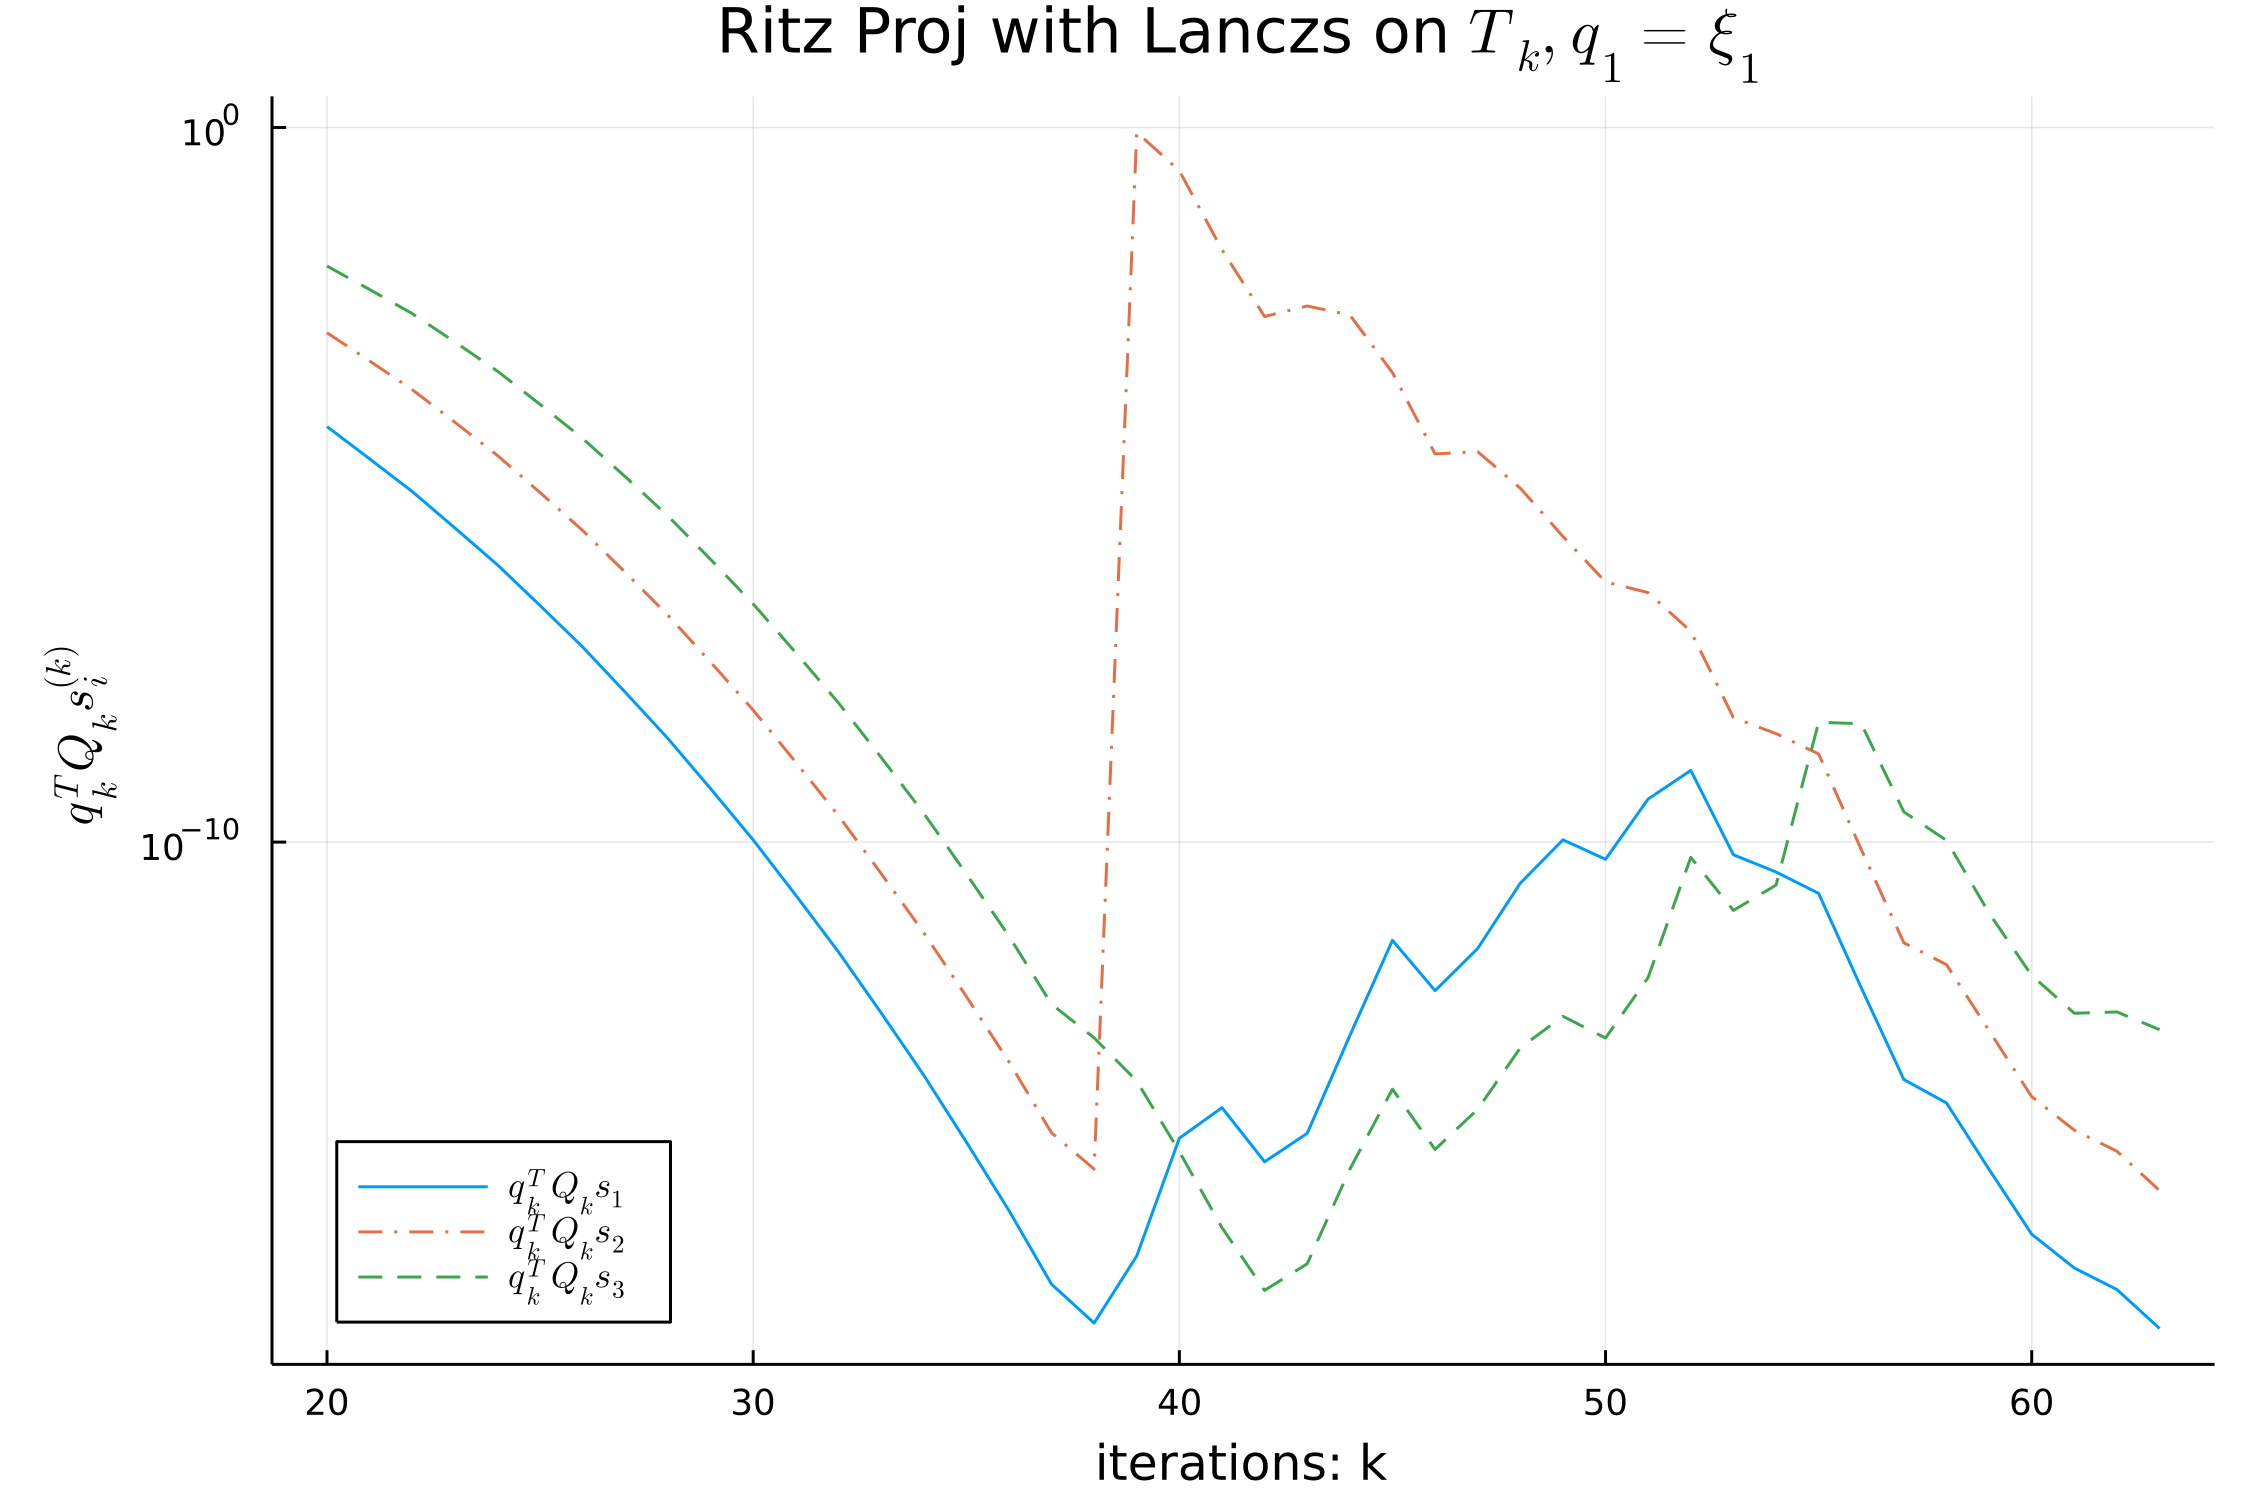
\includegraphics[width=14cm]{ritz_proj_tridiagonal.png}
                \caption{The projection of most recent Lanczos vector $q_k$ onto the first 3 Ritz vectors: $Q_ks_i^{(k)}$ for $1\le i \le 3$, it's performed on a Tridiagonal matrix $T_k$ generated by finite precision lanczos with $q_1 = \xi_1$. }
            \end{figure}\label{fig:6}
            \begin{remark}[Convergence Bounds on Ritzvalues]
                The above presentation for the convergence of a Ritz Value and Ritz vector is an oversimplification. What happened is complicated. The characteristic polynomial of $T_k$ minimizes under some weighted measured, hence the ritz values tends to approximate the eigenvalues of A, but this characteristic alone cannot dictate the way certain Ritzvalues converges.
                \par
                It's not always the case that $\theta_1^{(j)}$ for example, it's the best approximation for $\lambda_1$ of $A$, and it's especially true when iterations $j$ is relative small compare to $n$. The theoretical importance is to find an interval of how far are the $\lambda_i$ from $\theta_{i'}^{(k)}$, where $\lambda_i$ denotes the actual eigenvalue in $A$ where the Ritz value $\theta_{i'}^{(k)}$ is trying to approximate. The bound for the Ritz interval was refined by Y. Saad back in 1980\cite{paper:saad_ritz_convergence} and first discovered by Shmuel Kaniel back in 1966\cite{paper:kaniel1966}. 
            \end{remark}
    \subsubsection{Greenbaum's Tiny Interval Experiments}
        A smarter way of looking at the phenomenon of ghost eigenvalues (\hyperref[fig:2]{figure \ref*{fig:2} left}) is to take advantage of the clustering of the ghost eigenvalues and think of them as the eigenvalues of a potentially a larger matrix, denoted as $\tilde{A}$ whose eigenvalues are clustered around the eigenvalues of $A$ within a tiny interval. The idea is if we perform exact Lanczos on $A$, then we get similar results for applying floating-point Lanczos on $\tilde{A}$. Simply put, due to the effect of round of errors, the floating-point Lanczos iterations can't see the spectrum of $A$ clearly and instead, it sees $\tilde{A}$ whose eigenvalues are smeared out version of $A$, and there are many of them clustered around. More specifically, assuming $A$ has eigenvalues: $\lambda_1, \cdots, \lambda_n$, the eigenvalues of $\tilde{A}$ lies in: 
        \begin{align}
            \bigcup_{n = 1}^n[\lambda_i - \delta, \lambda_i + \delta]
        \end{align}
        As a result, running an exact Lanczos/CG on $\tilde{A}$ produces similar convergence compared to the floating-point version of the algorithm. Experiments where conducted by A. Greenbaum and Z. Strakos in 1992\cite{paper:greenbaum_tiny_interval_experiments}. Here, we reproduce the experiments on CG and check on the convergence rate of the algorithm. 
        \par
        To reproduce the effects, The same matrix paramaterized by $\rho$ back in \hyperref[eqn:paramaterized_experiment_matrix]{matrix \ref*{eqn:paramaterized_experiment_matrix}}. The tiny intervals are set by me via trials and errors. For the experiments, we set $\delta = \text{2e-5}\Vert A\Vert \epsilon$ where $\epsilon$ is the machine epsilon for Float64; and 100 equally spaced eigenvalues on the spectrum for the matrix $\tilde A$ are clustered inside of the tiny intervals. The right hand side vector $b,\tilde b$ are chosen to be a vector of all ones. The matrix $A$ is chosen to be $64 \times 64$, and hence $\tilde A$ is $6400 \times 6400$. 
        \par
        Both exact and float CG are run and terminates onece $\frac{\Vert e_k\Vert_A}{\Vert e_0\Vert_A}$ is less than $10^{-10}$. By exact CG I mean CG with full reorthogonalizations. 
        \begin{figure}[H]
            \centering
            \begin{subfigure}[H]{12cm}
                \centering
                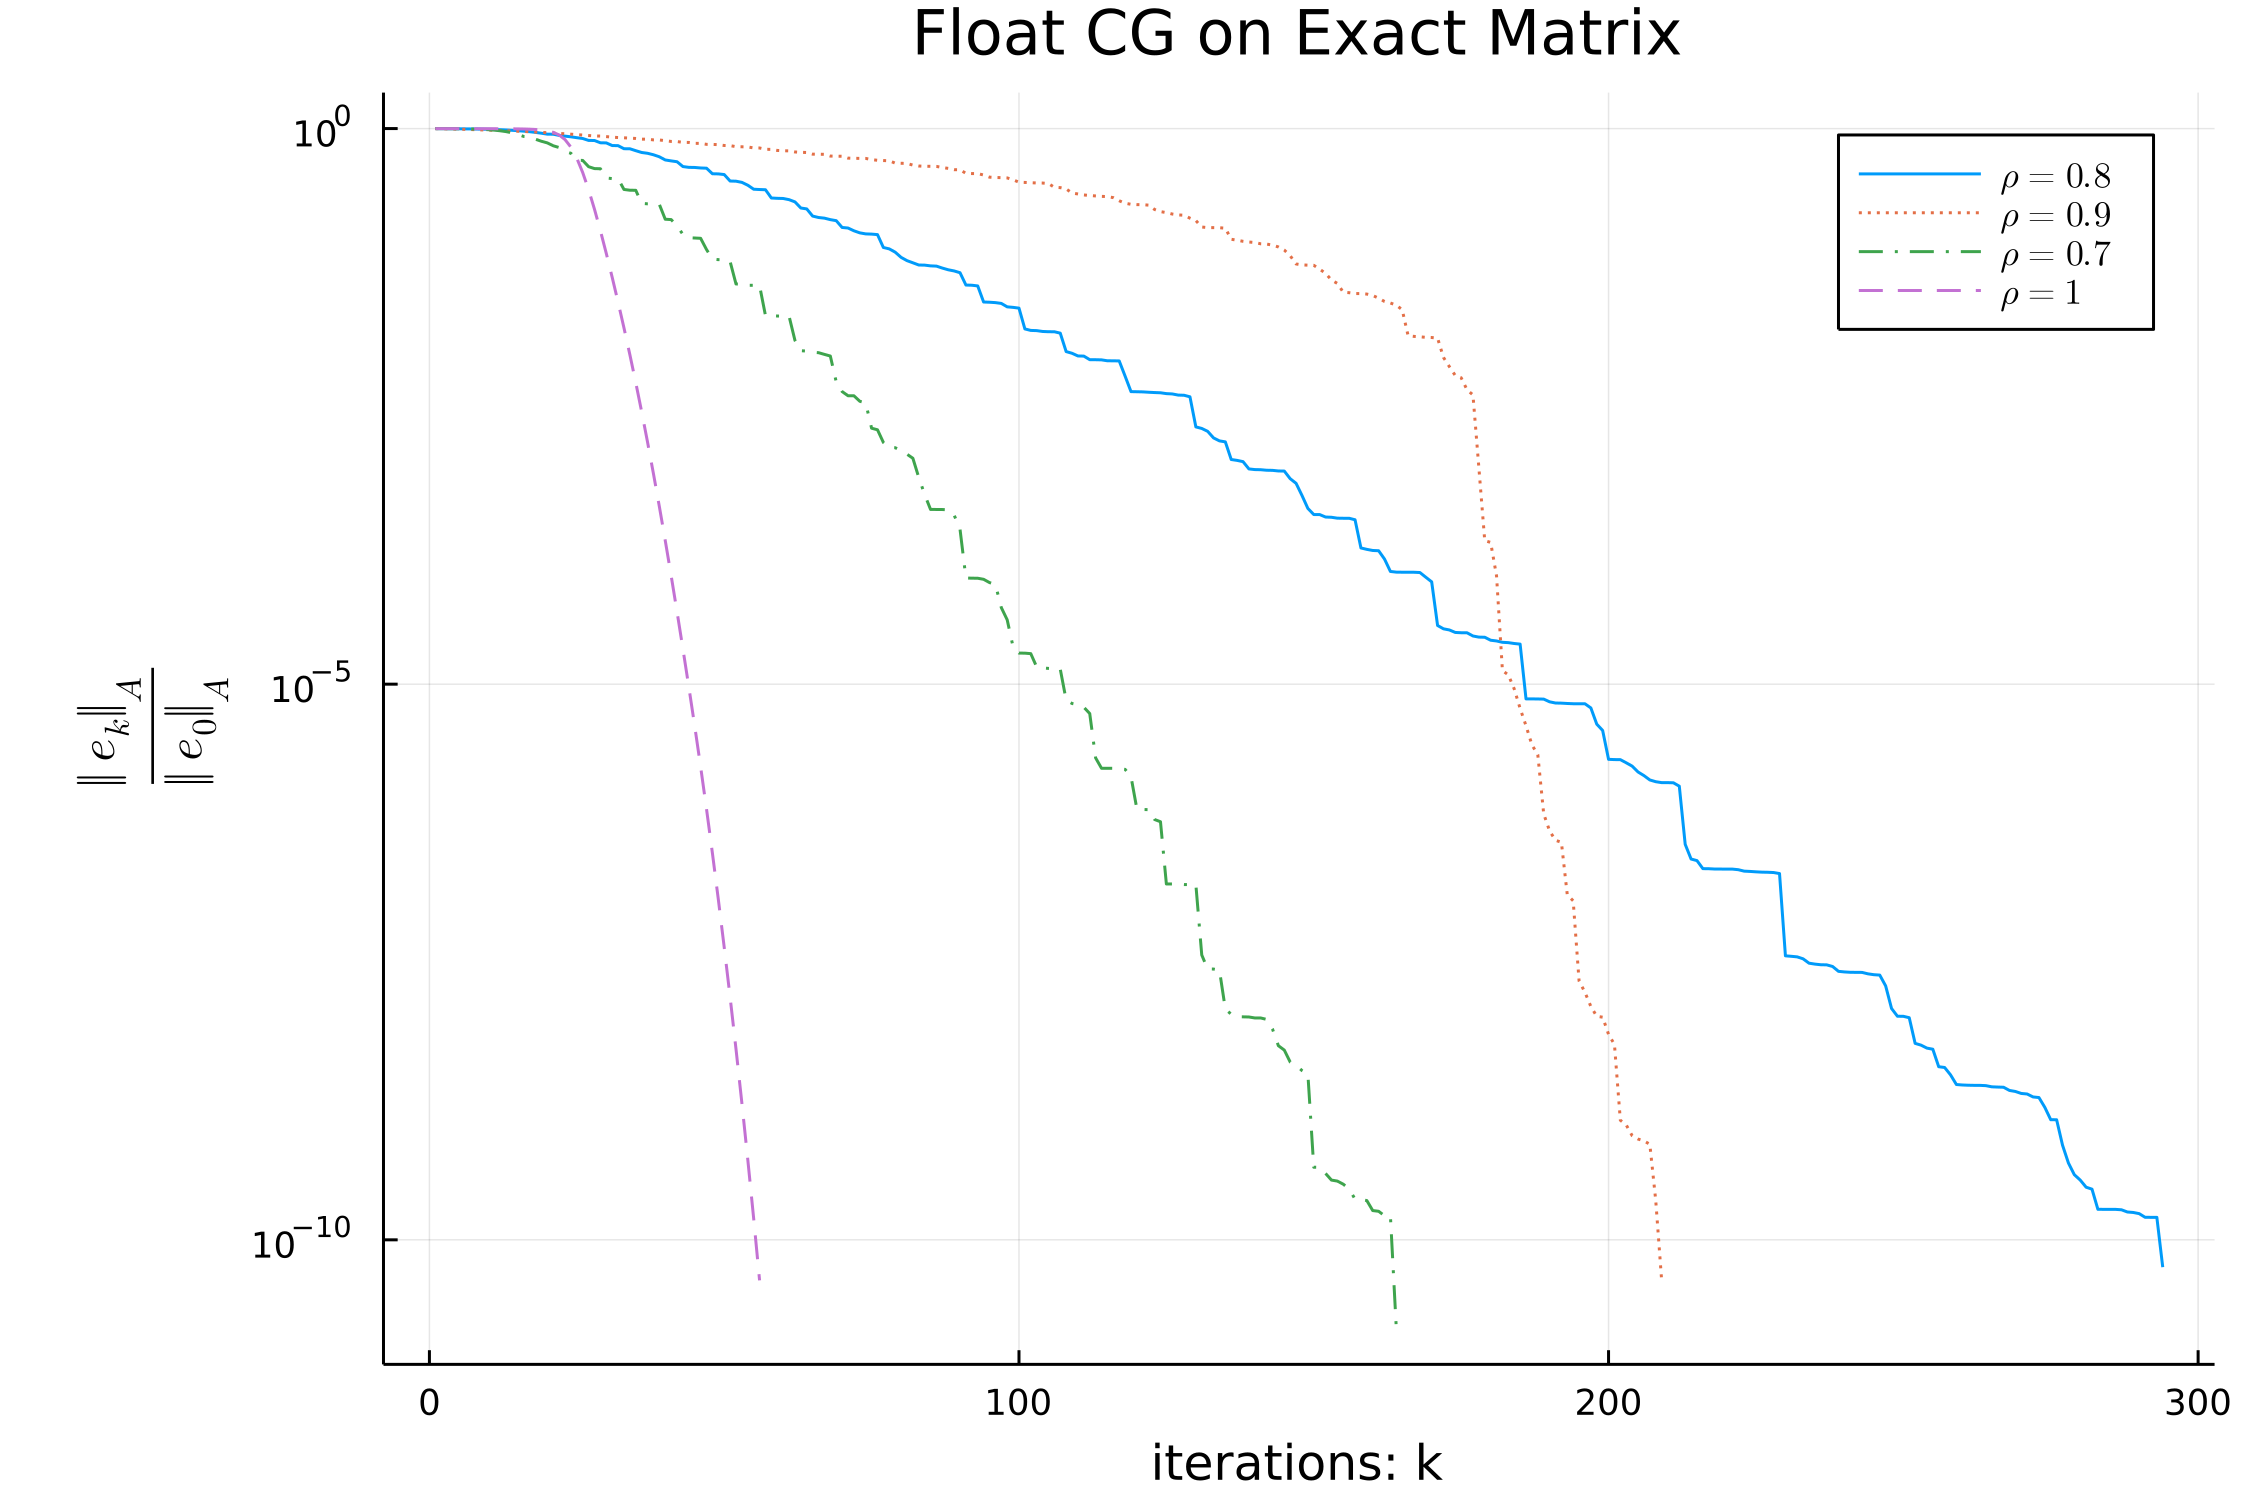
\includegraphics[width=12cm]{floats_cg_on_exact_matrix.png}
                \caption{Applying CG without re-orthogonalizations on $Ax = b$, the original matrix without the tiny intervals. }
                \label{fig:7.1}
            \end{subfigure}
            \\[2em]
            \begin{subfigure}[H]{12cm}
                \centering
                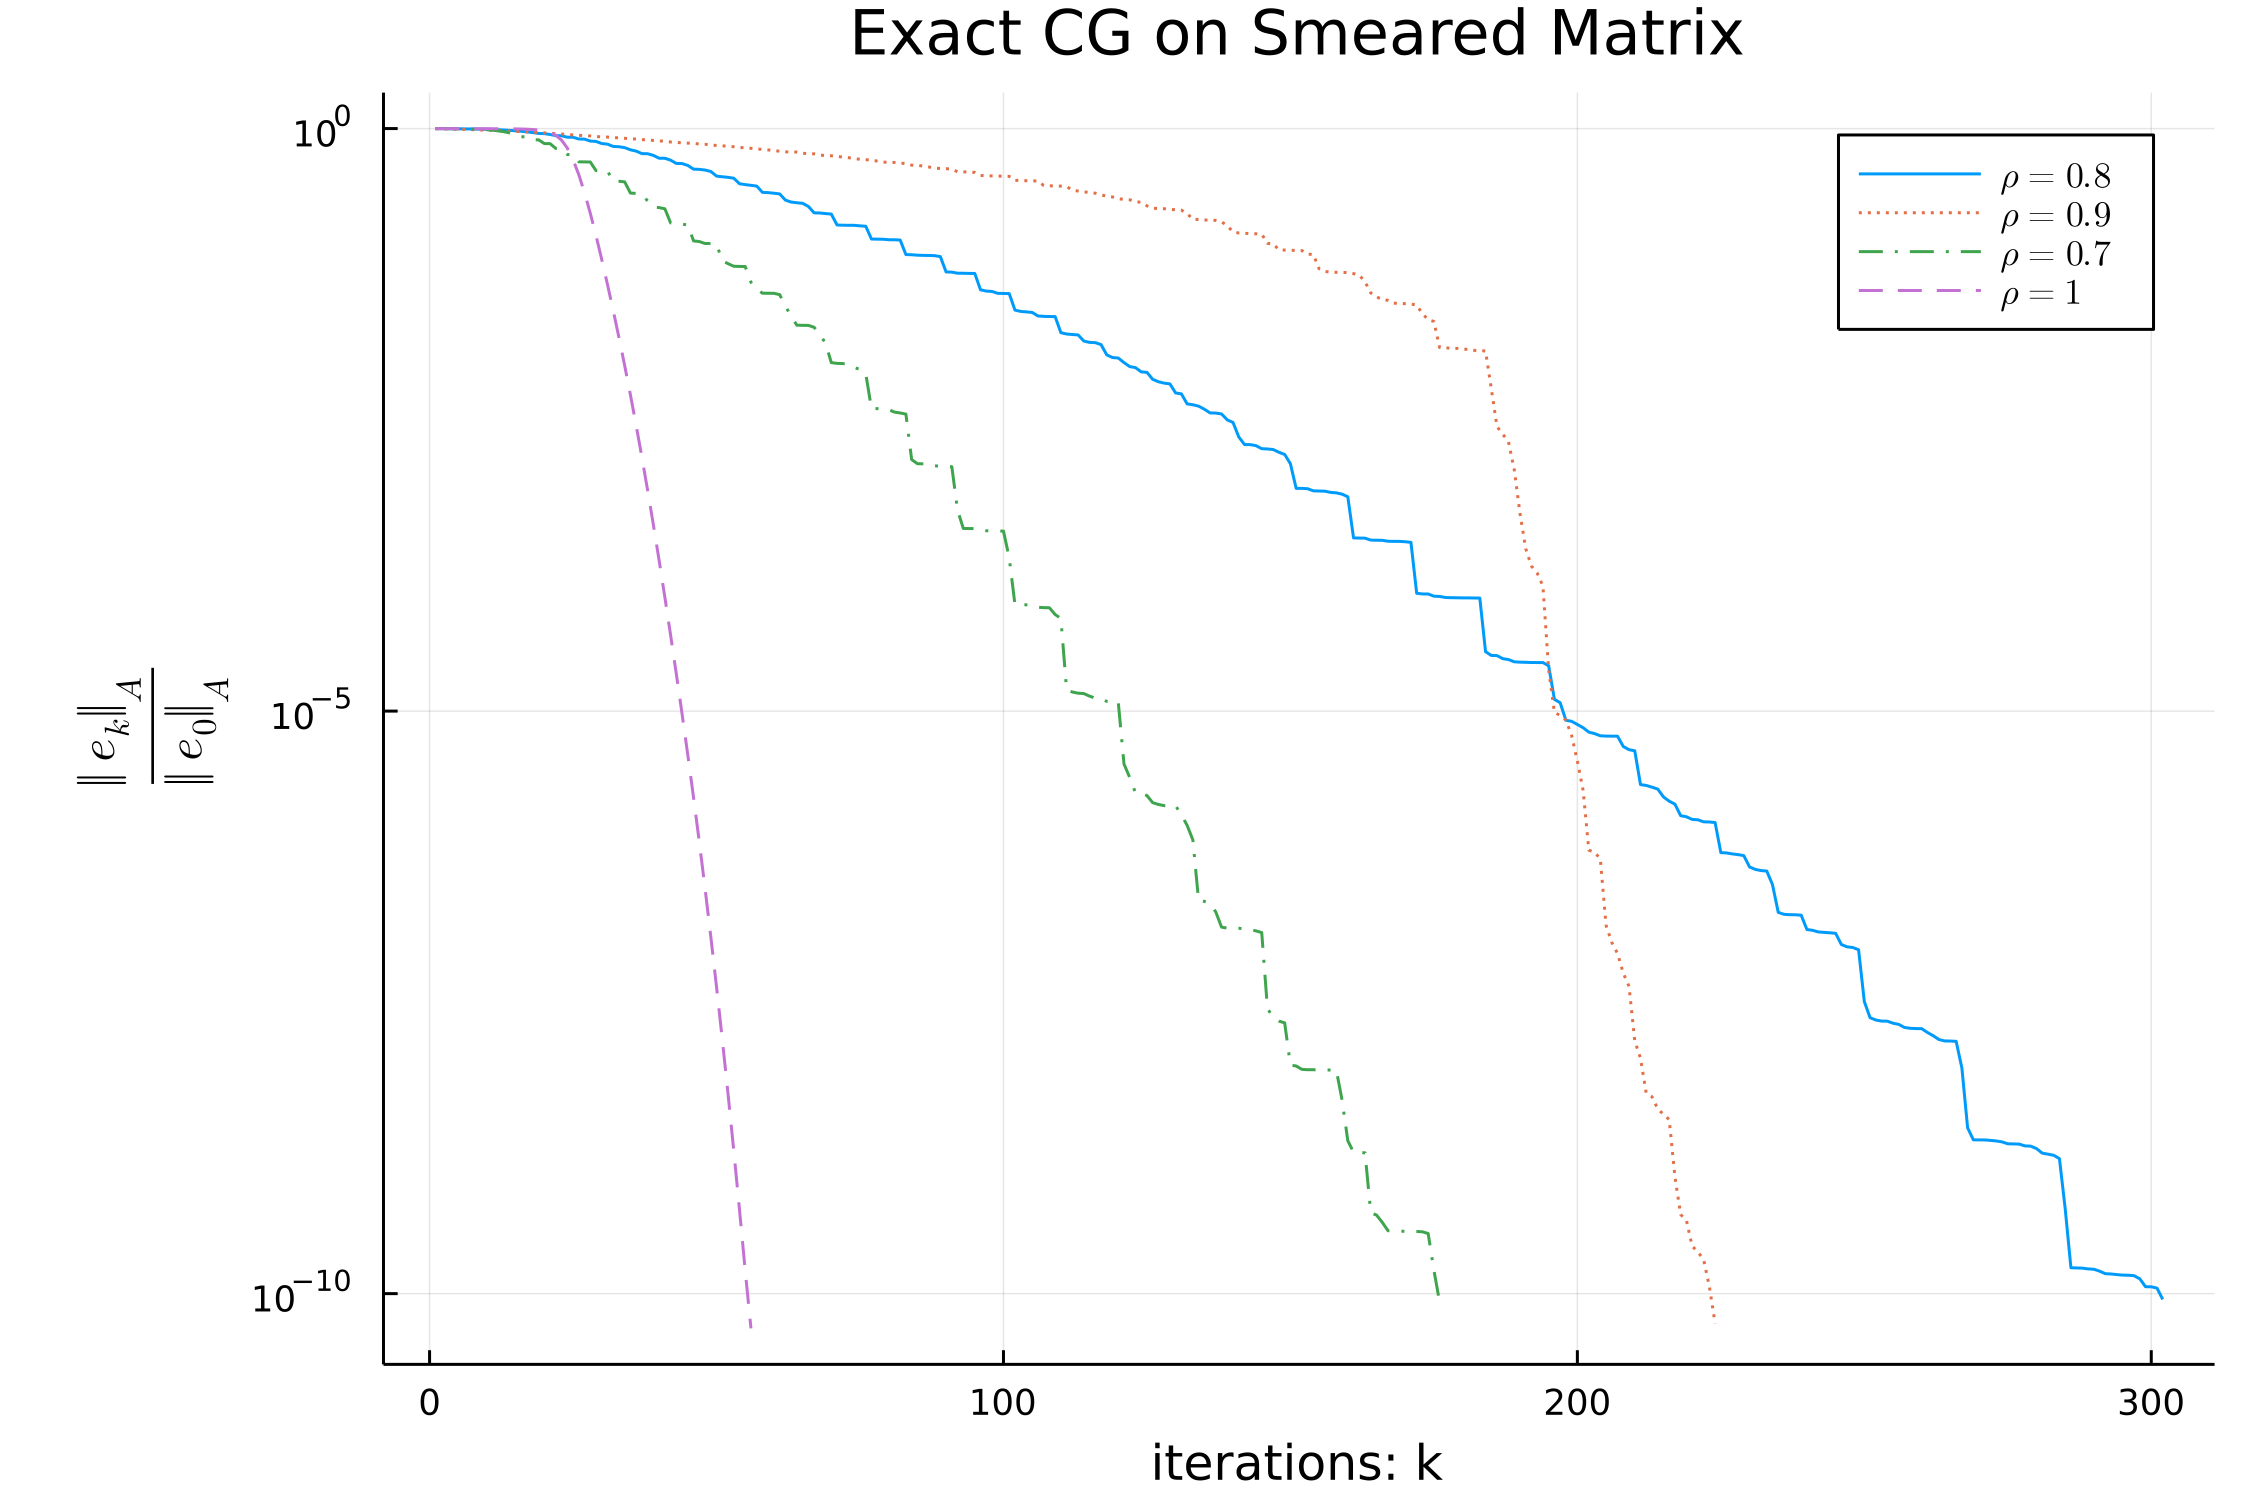
\includegraphics[width=12cm]{exact_cg_on_smeared_matrix.png}
                \caption{Applying CG with full re-orthogonalizations on $\tilde Ax = \tilde b$. $\tilde A$ has tiny intervals. }
                \label{fig:7.2}
            \end{subfigure}
            \caption{}\label{fig:7}
        \end{figure}
        The results of the experiments are plotted out in \hyperref[fig:7]{fig \ref*{fig:7}}. For a tolerance of $10^{-10}$ on the relative energy norm of the error, we reproduced the behaviors of the CG without re-orthogonalizations using the tiny intervals ideas. In \hyperref[fig:7.1]{fig \ref*{fig:7.1}} is the CG without any re-orthogonalizations applied on $Ax = b$ for different values of $\rho$, and in \hyperref[fig:7.2]{fig \ref*{fig:7.2}}, it's the convergence of the CG with full re-orthogonalizations on the system $\tilde A x = \tilde b$. 
        
        \begin{remark}[Optimal in Another Measure, and Open Questions]
            The idea of tiny intervals allows for a good predictions for the behaviors of CG and Lanczos when finite precision arithemtic is involved. The underlying mechanism was shown by Greenbaum in 1989\cite{paper:greenbaum1989}. The Lanczos iterations generates tridiagonal matrix whose characteristic polynomial is orthogonal under a discrete measure at eigenvalues of $A$ weighted by the vector $(U^Hq_1)^2$, ( \hyperref[prop:trid_char_poly_orthogonal]{appendix item \ref*{prop:trid_char_poly_orthogonal}}), however under finite arithmetic, they are no longer orthogonal under the original measure but instead, they are orthogonal under a new measured for some tiny intervals around the eigenvalues of $A$. 
            \par
            It's hypothesized that the tiny intervals are fixed and wrt to the number of iterations, however no current bounds are tight enough to show that's true. 
        \end{remark}
    

    \subsection{Another Paige's Theorem}
        Another Paige theorem highlights the systematic ways of Ritz vector losing orthognality. The theorem is stated in C.C Paige 1980 3.13\cite{paper:paige1980}, a more thorough proof is presented in Demmel's Book\cite{book:demmel997}. We present the thorough proof here for the sake of appreciation. 
        \par
        The theorem highlights two facts. Firstly is the loss of orthogonality of Lanczos Vector when $\beta_k, (v_i)_k^{(k)}$ is small. The second is that the projection of the Lanczos vectors $q_{k + 1}$ onto the converged Ritz vectors increases when $\beta_k, (v_i^{(k)})_k$ is small. It tells us that when under floating point arithematic, converged Ritz vector leads to lost of orthogonality of Lanczos vector, and they lose orthogonality along the direction of the converged Ritz vectors. 
        \begin{theorem}[Another Paige's Theorem]
            \begin{align}
                (y_i^{(k)})^Tq_{k + 1} &= \frac{\mathcal O(\epsilon \Vert A\Vert)}{\beta_k (v_i)_k}    
                \\
                y_i^{(k)} &:= Q_kv_i
            \end{align}
            And we define the following quantities: 
            \begin{align}
                T_k &:: \text{Tridiagonal at step k of Lanczos}
                \\
                Q_k &:: \text{Orthogonal matrix at step k of Lanczos}
                \\
                V_k = [v_1^{(k)}\;  v_2^{(k)}\; \cdots \; v_k^{(k)}] &:: \text{Eigen Matrix for } T_k
                \\
                \theta_i^{(k)} &:: \text{the eigenvalues for }v_i^{(k)}, \text{ Ritz Value}
                \\
                \Lambda_k &:: \text{Diagonal eigenvalues matrix for }T_k
                \\
                F_k &::\text{The floats error matrix from Lanczos recurrence}
                \\
                \epsilon &:: \text{The machine Epsilon}
            \end{align}
        
        \end{theorem}
        \begin{proof}
            For simplicity, we ignore all the subscript goes under $Q_k, q_{k + 1}, T_k, F_k, v_i^{(k)}, y_i^{(k)}$. Starting with the Lanczos recurrences under floating point arithmetic: 
            \begin{align}
                AQ &= AT + \beta q\xi_k^T + F
                \\
                Q^TAQ &= Q^TQT + Q^T\beta q\xi_k^T + Q^TF
                \\
                Q^TAQ &= (Q^TQT + Q^T\beta q\xi_k^T + Q^TF)^T
                \\
                &= T^TQ^TQ  + \beta\xi_k q^T Q + F^TQ
            \end{align}
            The third line (5.5.12) is obtained by the fact that $Q^TAQ$ is symmetric. Takes the difference between the second line (5.5.11) and the third line(5.5.12) from above, we have: 
            \begin{align}
                \mathbf{0} = (Q^TQT - T^TQ^TQ) + \beta(Q^Tq\xi_k^T - \xi_k q^TQ) + (Q^TF - F^TQ)
            \end{align}
            Here, we make the approximation that $\langle q_i, q_j\rangle = 0$ when $|i - j| \le 2$ throughout the rest of the derivation, in theory, it should be $\mathcal{O}(\epsilon)$, but we ignore error of orthgonalizing the vector $q_{j + 1}$ against the vector $q_j, q_{j - 1}$ because it's small enough and doesn't change the final result. 
            \par
            As a result we obtained the factorization $Q^TQ = I + C^T + C$ where the matrix $C$ is lower triangular with diagonal and sub-diagonals being all zeros, representing the Lanczos vectors losing orthogonality. Which means that $C^T + C$ is a matrix with zeros on the tridiagonal parts and all other entries are the floating point errors from lost of orthogonality. We proceed to simplify the first term from (5.5.14): 
            \begin{align}
                    Q^TQT - T^TQ^TQ &= (I + C^T + C)T -T^T (I + C^T + C)
                    \\
                    &= T + C^TT + CT - T^T - T^TC^T - T^TC
                    \\
                    &= (CT - TC) + (C^TT - TC^T)
            \end{align}
            $CT$ is strictly lower triangular, $TC$ is strictly lower triangular as well. This is true because a tridiagonal matrix only encodes interactions between adjacent rows/columns, and $C$ has zeros on it's tridiagonal parts.
            \par
            $\xi q^TQ$, adding back the subscript we have: $\xi_k q_{k + 1}^TQ_k$, observe that $\xi_k q_{k + 1}^T$ is a matrix whose last row is $q_{k + 1}^T$. And because of the way that $q_{k + 1}$ is orthogonalized, the last 2 elements of the last row of $\xi_k q_{k + 1}Q_k$ is zero.
            \par
            Consider $\xi q^TQ$ after adding back the subscript we have: $\xi_k q_{k + 1}^TQ_k$, observe that $\xi_k q_{k + 1}^T$ is a matrix whose last row is $q_{k + 1}^T$. And because of the way that $q_{k + 1}$ is orthogonalized, the last 2 elements of the last row of $\xi_k q_{k + 1}Q_k$ is zero, which is strictly lower triangular. Using the results we have we reconsider: 
            \begin{align}
                \mathbf{0} &= (Q^TQT - T^TQ^TQ) + \beta(Q^Tq\xi_k^T - \xi_k q^TQ) + (Q^TF - F^TQ)
                \\
                \mathbf{0}&= 
                -\underbrace{(CT - TC)}_{\text{strict tril}} + \underbrace{(C^TT - TC^T)}_{\text{strict triu}} + \beta(\underbrace{Q^Tq\xi_k^T}_{\text{strict triu}} - \underbrace{\xi_k q^TQ}_{\text{strict tril}}) - (Q^TF - F^TQ)
                \\\implies
                \mathbf{0} &= (CT - TC) - \beta \xi_k q^TQ + \underbrace{\text{tril}(Q^TF - F^TQ)}_{=:L}
            \end{align}
            From the second line (5.5.19) to the third line (5.5.20), we take $\text{triu}$ on both side of the equation. Now consider multiplying by $v^T(\bullet)v$ for each terms in the above expression and we have: 
            \begin{align}
                v^T(CT - TC)v &= v^TCTv - v^TTCv
                \\
                &= 
                v^TC\theta v - \theta v^TCv
                \\
                &= 0
            \end{align}
            Therefore we are left with the equality: 
            \begin{align}
                v^T\beta\xi_k q^TQv &= v^TLv
                \\
                (\beta(v)_k)(q^TQv) &= v^T Lv
                \\
                \beta(v)_kq^Ty &= v^TLv
            \end{align}
            Adding back the subscripts we have: $\beta_k (v_i^{(k)})_k q_{k + 1}^Ty_i^{(k)} = v^TLv$, notice that $|v^TLv| =\mathcal O (\Vert L\Vert) = \mathcal{O}(\Vert Q^TF - F^TQ\Vert) = \mathcal O(\epsilon \Vert A\Vert)$, which obtains the formula for this theorem. 
        \end{proof}
        \begin{remark}[Mitigating the Lost of Orthogonality]
            For Conjugate Gradient, there is little needs for asserting orthogonality and A-Orthogonality between the vectors $r_k$ and $p_k$ unless ones need to emulate the behaviors of the algorithm under exact arithmetic. The Lanczos algorithm is sometimes used for symmetric eigenvalues problem, and in that case, making sure $Q_k$ is orthogonal will eliminate ghost eigenvalues. Fortunately, there are ways where one can avoid the computational expense of full re-organization to eliminate ghost eigenvalues. 
            \par
            In practice, there exists Lanczos iterations that detects for lost of orthogonality between Lanczos vector and performs selective re-orthogonalizations of Lanczos vectors against Ritz vectors. The implementations of such algorithm appears first back in 1979 by B. N. Parlett and D. S. Scott\cite{article:lanso}. Later however, more sophisticated algorithms arised, and the state of the art Lanczos algorithm implementation can be found in a 1992 paper by Grimes, Roger G. and Lewis, John G. and Simon, Horst D.\cite{article:shifted_block_lanczos}. 
        \end{remark}
        
\begin{appendices}
    
    \section{Useful Lemmas}
        \subsection{Relative Energy Norm and Relative 2-Norm Conversions}
        \begin{lemma}[Relative Energy Norm and Relative 2-Norm Conversions]\label{lemma:Relative_Energy_Norm_and_Relative_2_Norm_Conversions}
            Let $A$ be a Positive Symmetric Positive Definite Matrix, then it can be said that: 
            $$
            \frac{\Vert A x\Vert}{\Vert Ay \Vert} \le \kappa(A)\frac{\Vert 
            x\Vert_A}{\Vert y \Vert_A}
            $$
        \end{lemma}
        \begin{proof}
            From the definition of included 2-norm of matrices, assuming that $\lambda_1$ is the minimum eigenvalue of the matrix $A$, and $\lambda_n$ the maximum, and the fact that matrix $A$ has factorization $A^{1/2}A^{1/2}$: 
            \begin{align}
                \lambda_1 \Vert x \Vert 
                &\le \Vert Ax\Vert 
                \le \lambda_2 \Vert x\Vert
                \\
                \sqrt{\lambda_1} \Vert x\Vert 
                & \le \Vert A^{1/2}x\Vert \le \sqrt{\lambda_n}\Vert x \Vert
                \\
                \implies
                \sqrt{\lambda_1} & \le \frac{\Vert Ax\Vert}{\Vert A^{1/2}x \Vert} 
                \le \sqrt{\lambda_n}
            \end{align}
            Consider another vector $y$: 
            \begin{align}
                \sqrt{\lambda_1} \le \frac{\Vert Ay\Vert}{\Vert A^{1/2}y \Vert} \le \sqrt{\lambda_n}
            \end{align}
            Combining the two we have: 
            \begin{align}
                \sqrt{\lambda_1}\frac{\Vert Ax\Vert}{\Vert A^{1/2}x \Vert} 
                & \le \sqrt{\lambda_n}\sqrt{\lambda_1}
                \\
                \sqrt{\lambda_1}\sqrt{\lambda_n}& \ge \sqrt{\lambda_n} \frac{\Vert Ay\Vert}{\left\Vert
                    A^{1/2}y
                \right\Vert}
                \\
                \implies 
                \sqrt{\lambda_1}\frac{\Vert Ax\Vert}{\Vert A^{1/2}x \Vert} & \le 
                \sqrt{\lambda_n} \frac{\Vert Ay\Vert}{\left\Vert
                    A^{1/2}y
                \right\Vert}
                \\
                \frac{\Vert Ax\Vert}{\Vert A^{1/2}x\Vert} &\le 
                \sqrt{\kappa(A)} 
                \frac{\Vert Ay\Vert}{\Vert A^{1/2}y\Vert}
                \\
                \frac{\Vert Ax\Vert}{\Vert Ay\Vert} &\le 
                \sqrt{\kappa(A)} 
                \frac{\Vert A^{1/2}x\Vert}{\Vert A^{1/2}y\Vert}
                \\
                \frac{\Vert Ax\Vert}{\Vert Ay\Vert} &\le 
                \sqrt{\kappa(A)} 
                \frac{\Vert x\Vert_A}{\Vert y\Vert_A}
            \end{align}
        \end{proof}
    \section{Theorems, Propositions, Proofs}
        \subsection{Krylov Subspace Grade Invariant Theorem}
            \begin{prop}[Krylov Subspace Grade Invariant Theorem]\label{prop:Krylov_Subspace_Grade_Invariant_Theorem}
                Once the subspace becomes linearly dependent, the subspace becomes invariant. 
            \end{prop}
            \begin{proof}
                \begin{align}
                    & K_k = \begin{bmatrix}
                        b & AB & \cdots & A^{k - 1}b
                    \end{bmatrix}
                    \\
                    & K_k \text{ Lin Dep} \implies A^{k-1}b = K_{k - 1}c_k
                    \\
                    & \implies 
                    AK_k = K_k
                        \underbrace{\begin{bmatrix}
                            e_2 & \cdots & e_k & c_k
                        \end{bmatrix}}_{:= C_k}
                    \\
                    & \implies 
                    A^2K_k = AK_kC_k = K_kC_k^2
                \end{align}
                $A^2K_k$ will span the same space as the range of the matrix $K_k$.
            \end{proof}
        \subsection{Cauchy Interlace Theorem for Tridiagonal Symmetric Matrices}
            \begin{theorem}[Cauchy Interlace Theorem for Tridiagonal Symmetric Matrices]\label{theorem:cauchy_interlace}
                Let $T_k$ be a $k\times k$ symmetric tridiagonal matrix, then its top left upper submatrix: $T_{k-1}=(T_k)_{:k - 1, :k -1}$ has eigenvalues interlaced between the eigenvalues of $T_k$. Denotes all $k$ eigenvalues of $T_k$ as $\theta_i^{(k)}$, and all $k - 1$ eigenvalues of $T_{k - 1}$ as $\theta_i^{(k - 1)}$. Order them so that: $\theta_1^{(k - 1)} \le \cdots, \le \theta_i^{(k - 1)}$, similarly: $\theta_1^{(k)}\le \cdots \le \theta_i^{(k)}$, then: 
                \begin{align}
                    & \theta_{k}^{(k)} \ge \theta_{k - 1}^{(k - 1)}
                    \\
                    & \theta_{1}^{(k)} \le \theta_{1}^{(k - 1)}
                    \\
                    & \theta_{i -1}^{(k - 1)} \le \theta_{i}^{(k)} \le \theta_{i}^{(k - 1)}
                \end{align}
                Theorem taken from first chapter of Greenbuam's book\cite{book:greenbaum} and it's adapted for symmetric tridiagonal matrix. 
            \end{theorem}
        \subsection{Orthogonal Polynomials and Lanczos}
            \begin{prop}[Orthogonal Polynomials and Lanczos]\label{prop:Orthogonal_Polynomials_and_Lanczos}
                The Lanczos algorithm generates orthogonaly polynomial under a discrete weighted measure under the eigenvalues of matrix $A$, which is also the Lanczos vector $q_k$ represented under the Krylov subspace. 
            \end{prop}
            \begin{proof}
                Let $V_k^HAV_k = T_k$ be the tridiagonalization resulted from Lanczos algorithm and we assume exact arithematic, using the fact that each lanczos vector $q_k$ is an element from the Krylov subspace, we can represent it as a matrix polynomial multiplied by $q_k$: 
                \begin{align}
                    v_{m + 1} &= q_{m}(A)v_1 \in \mathcal{K}(A|v_1) \quad \forall\; m \le k - 1
                    \\
                    \exists\; q_{i} &\in \mathcal{P}_{i - 1}: v_i = q_{i - 1}(A) v_1
            \end{align}
            Since the exact arithematic generates orthogonal lanczos vectors, let's consider $v_i, v_j$ being represented by polynomial $\phi, \varphi$, then we have:
            \begin{align}
                \langle v_i, v_j\rangle &= 0 
                \\
                \langle\phi(A)v_1, \varphi(A)v_1 \rangle &= 0
                \\
                \langle U\phi(\Lambda)U^Hv_1, U\varphi(\Lambda)U^Hv_1\rangle &= 0
                \\
                \text{Let: }f_1 &= U^Hv_1 \text{ Then: }
                \\
                \langle U\phi(\Lambda)f_1, U\varphi(\Lambda)f_1\rangle &= 0
                \\
                \langle \phi(\Lambda)f_1, \varphi(\Lambda)f_1\rangle &= 0
                \\
                \sum_{i = 1}^{n} (f_1)_i^2\phi(\lambda_i)\varphi(\lambda_i) &= 0
            \end{align}
            Therefore the polynomials $\phi, \varphi$ are orthogonal under the discrete measure over eigenvalues of $A$ weighted by the vector $(f_1)^2$. 
        \end{proof}
        \subsection{Recursion of the Symmetric Tridiagonal Matrix Determinant}
            \begin{prop}[Recursion of the Symmetric Tridiagonal Matrix Determinant]\label{prop:Recurrence_of_the_Symmetric_Tridiagonal_Matrix_Determinant}
                Let $T_k$ be a symmetric tridiagonal matrix $\in \mathbb{R}^{k\times k}$ with $\alpha_i$ on its diagonal and $\beta_i$ on its subdiagonal. Recursively, we define $T_{k - i} = (T_{k})_{1:k - i, 1:k - 1}$. Using $|\cdot|$ to denote the determinant of a matrix, we have the recurrence relation: 
                $$
                    |T_k| = \alpha_k|T_{k - 1}| - \beta_{k - 1}^2|T_{k - 2}|
                $$
            \end{prop}
            \begin{proof}
                Using the notation of $e_{k}^{(m)}$ to denote the $k^{th}$ standard basis vector in $\mathbb{R}^m$, consider the Block Matrix: 
                \begin{align}
                    T_k &= \begin{bmatrix}
                        T_{k - 2} & \beta_{k - 2}e_{k - 1}^{(k - 2)} & 
                        \\
                        \beta_{k - 2}e_{k - 2}^{(k - 2)T} & \alpha_{k - 1}  & \beta_{k - 1}e_{k - 1}^{(k - 1)}
                        \\
                        & \beta_{k - 1}e_{k - 1}^{(k - 1)T} & \alpha_k&
                    \end{bmatrix}
                \end{align}
                Now, we use the Laplace Expansion to figure out the determinant we are expanding the Laplace Expansion on the last row of $T_k$
                \begin{align}
                    &|T_k| = (-1)^{k+(k - 1)}\beta_{k - 1} \left|\begin{bmatrix}
                        T_{k - 2} & 
                        \\
                        \beta_{k - 2}e^{(k - 2)T}_{k - 2} & \beta_{k - 1}e_{k - 1}^{(k - 1)}
                    \end{bmatrix}\right|&
                     + 
                    (-1)^{2k} \alpha_k
                    \left|
                        \underbrace{\begin{bmatrix}
                            T_{k - 2} & \beta_{k - 2}e_{k - 1}^{(k - 2)} 
                            \\
                            \beta_{k - 2}e_{k - 2}^{(k - 2)T} & \alpha_{k - 1}
                        \end{bmatrix}}_{=T_{k - 1}}
                    \right|
                    \\
                    &(-1)^{2k - 2}\beta_{k - 1}|T_{k - 2}| 
                    = 
                    \left|\begin{bmatrix}
                        T_{k - 2} & 
                        \\
                        \beta_{k - 1}e^{(k - 2)T}_{k - 2} & \beta_{k - 2}e_{k - 1}^{(k - 1)}
                    \end{bmatrix}\right|&
                \end{align}
                Substituting the last equation back to the first equation of the first term. 
                \begin{align}
                    |T_k| &= 
                    (-1)^{2k - 2 + 2k - 1}\beta_{k - 1}^2|T_{k - 2}| + \alpha_k|T_{k - 1}|
                    \\
                    &= -\beta_{k - 1}^2|T_{k - 2}| + \alpha_k|T_{k - 1}|
                \end{align}
            \end{proof}
        \subsection{Recurrence of the Characteristic Polynomial of a Symmetric Tridiagonal Matrix}
            \begin{theorem}[Recurrence of the Characteristic Polynomial of a Symmetric Tridiagonal Matrix]
            \label{theorem:Recurrence_of_the_Characteristic_Polynomial_of_a_Symmetric_Tridiagonal_Matrix}
            The characteristic polynomial of a symmetric tridiagonal matrix satisfies the recurrences: 
            $$
            \begin{cases}
                p_k(x) = - \beta_{k - 1}^2 p_{k - 2}(x) + (\alpha_k - x)p_{k - 1}(x)
                \\
                p_0(x) = 1
                \\
                p_{-1}(x) = 0
            \end{cases}
            $$
            Where, $p_k(x) = |T_k - xI|$, and $p_{k - 1}(x) :=|(T_k)_{1:k - 1, 1:k - 1}|$, and $p_{k - 2} = |(T_k)_{1:k - 2, 1:k - 2}|$. 
            \end{theorem}
            \begin{proof}
                Using \hyperref[prop:Recurrence_of_the_Symmetric_Tridiagonal_Matrix_Determinant]{Proposition \ref*{prop:Recurrence_of_the_Symmetric_Tridiagonal_Matrix_Determinant}}, but replacing $\alpha_k$ to be $\alpha_k - x$ due to the shifting introduced by $T_k - xI$, then: 
                \begin{align}
                    |T_k - Ix| &= (\alpha_k - x)|T_{k - 1} - xI| -\beta_{k - 1}^2|T_{k - 2} - Ix|
                    \\
                    \implies
                    p_k(x) &= - \beta_{k - 1}^2 p_{k - 2}(x) + (\alpha_k - x)p_{k - 1}(x)
                \end{align}
                The recurrence is direct from the recurrences of the determinant of symmetric tridiagonal matrix, and a monic polynomial with degree zero is just $1$, therefore the base case matches up as well. 
            \end{proof}
        \subsection{Tridiagonal Characteristic Polynomials is Scaled Lanczos Orthgonal Polynomials}
            \begin{prop}[Tridiagonal Characteristic Polynomials is Scaled Lanczos Orthgonal Polynomials]\label{prop:trid_char_poly_orthogonal}
                The characteristic polynomial of $T_k$(with recurrence justified in \hyperref[theorem:Recurrence_of_the_Characteristic_Polynomial_of_a_Symmetric_Tridiagonal_Matrix]{Theorem \ref*{theorem:Recurrence_of_the_Characteristic_Polynomial_of_a_Symmetric_Tridiagonal_Matrix}}) is a scalar multiple of the polynomial that represents the lanczos vector $q_k$ under the Krylov Subspace (from \hyperref[prop:Orthogonal_Polynomials_and_Lanczos]{proposition \ref*{prop:Orthogonal_Polynomials_and_Lanczos}}). The relation is: 
                \begin{align}
                    \psi_j(x) = \left(\prod_{i = 1}^{j-1} \beta_i\right)^{-1}
                    (-1)^{j - 1}p_{j - 1}(x)
                    \quad \forall\; 1 \le j \le k
                \end{align}
            \end{prop}
            \begin{proof}
                To justify, we use the recurrence of the characteristic polynomial of the tridiagonal matrix together with the recurrence representing the $q_k$ Lanczos vector. Inductively we assume the above (B.6.1) is true up to $j$. Recall:
                \begin{align}
                    &\begin{cases}
                        \beta_j \psi_{j + 1} = 
                        (x - \alpha_j)\psi_j - \beta_{j - 1}\psi_{j -1}    
                        & \forall j \ge 2
                        \\
                        \psi_1 = 1
                        \\
                        \psi_0 = 0
                    \end{cases}
                    \\
                    &
                    \begin{cases}
                        p_j(x) = (\alpha_j - x)p_{j - 1}(x) - \beta_{j - 1}^2p_{j - 1}(x)    
                        &
                        \forall j \ge 1
                        \\
                        p_0(x) = 1 
                        \\
                        p_{-1}(x) = 0
                    \end{cases}
                \end{align}
                The base case matches up, consider: 
                \begin{align}
                    \beta_j\psi_{j + 1} &= (x - \alpha_j)\psi_j + \beta_{j - 1}\psi_{j - 1}
                    \\
                    &= (x - \alpha_j)\left(
                        \prod_{i = 1}^{j - 1}\beta_i
                    \right)^{-1}(-1)^{j + 1}p_{j - 1}
                    + 
                    \beta_{j - 1}\left(
                        \prod_{i = 1}^{j - 2}\beta_i
                    \right)^{-1}(-1)^{j}p_{j - 2}
                    \\
                    &= 
                    \left(
                        \prod_{i = 1}^{j - 2}\beta_i
                    \right)^{-1}
                    \left(
                        (x - \alpha_j)\beta_{j - 1}^{-1}(-1)^{j + 1}p_{j + 1}
                        + 
                        \beta_{j - 1}(-1)^jp_{j -2}
                    \right)
                    \\
                    &= 
                    \left(
                        \prod_{i = 1}^{j - 2}\beta_i
                    \right)^{-1}
                    (-1)^{j}
                    \left(
                        (\alpha_j - x)\beta_{j - 1}^{-1}p_{j + 1}
                        + 
                        \beta_{j - 1}p_{j -2}
                    \right)
                    \\
                    &=
                    \left(
                        \prod_{i = 1}^{j - 2}\beta_i
                    \right)^{-1}
                    (-1)^{j}\beta_{j - 1}^{-1}
                    \underbrace{\left(
                        (\alpha_j - x)p_{j + 1}
                        + 
                        \beta_{j - 1}^2p_{j -2}
                    \right)}_{=p_j(x)}
                    \\
                    &= 
                    \left(
                        \prod_{i = 1}^{j - 1}\beta_i
                    \right)^{-1}(-1)^{j + 2}p_j(x)
                    \\
                    \implies  \beta_j\psi_{j + 1} &= \left(
                        \prod_{i = 1}^{j - 1}\beta_i
                    \right)^{-1}(-1)^{j + 2}p_j(x)
                \end{align}
                Moves $\beta_{j}$ to the RHS and we proved the statement for $j + 1$ remains true. 
            \end{proof}
        \subsection{Irreducible Symmetric Tridiagonal Matrix}
            \begin{prop}\label{prop:Irreducible Symmetric Tridiagonal Matrix}
                The tridiagonal matrix $T_k$ generated by the Lanczos algoithm cannot have repeated eigenvalues. It's what referred to as a irreducible symmetric tridiagonal matrix in some literature. 
            \end{prop}
            \begin{proof}
                Let $T_k$ be symmetric tridiaognal $k\times k$ matrix, its all sub/super diagonals are nonzeros. Consider the submatrix $(T_k - \lambda I)_{2:k, 1:k-1}$ with the first row and last column removed. Regardless of $\lambda$, $(T_k - \lambda I)_{2:k, 1:k-1}$ whose diagonals are the sub diagonals of $T_k$, which is all non-zero. Hence $\text{det}((T_k - \lambda I)_{2:k, 1:k-1})\neq 0 \;\forall \lambda$. 
                \par
                The determinant of $(T_k - \lambda I)_{2:k, 1:k-1}$ is always nonzero implies that the full matrix $T_k - \lambda I$ has a rank of at least $k - 1$ for all $\lambda$; which implies that all roots of $\det(T_k - \lambda I)$ has algebraic multiplicity of strictly 1.
                \par
                Since the matrix is symmetric, it must be diagonalizable. For contradiction assuming that it has repeated eigenvalues and still diagonalizable, it must have repeated roots, which is a contradiction. Therefore all its eigenvalues are unique. 
            \end{proof}
        \subsection{From CG to Lanczos: The Proof}\label{sec:From_CG_to_Lanczos:The_Proof}
            We will break the proof into several parts. Firstly we address the base case, and then we address the inductive case to establish the parameters between the Tridiagonal matrix and $a_k, b_k$, finally we resolve the sign problem between the Lanczos vectors and the residual vectors. 
            \subsubsection{The Base Case}
                Right from the start of the CG iteration we have: 
                \begin{align}
                    r_0 &= p_0
                    \\
                    r_1 &= r_0 - a_0Ar_0
                    \\
                    Ar_0 &= a_0^{-1}(r_0 - r_1)
                    \\
                    Ar_0 &= \frac{\Vert r_0\Vert_A^2}{\Vert r_0\Vert^2}(r_0 - r_1)
                \end{align}
                Consider substituting $r_0 = \Vert r_0\Vert q_1, r_1 = -\Vert r_1\Vert q_2$, then: 
                \begin{align}
                    A\Vert r_0\Vert q_1 
                    &= \frac{\Vert r_0\Vert_A^2}{\Vert r_0\Vert^2}\left(
                        \Vert r_0\Vert q_1 + \Vert r_1\Vert q_2
                    \right)
                    \\
                    &= 
                    \frac{\Vert r_0\Vert_A^2}{\Vert r_0\Vert^2}\Vert r_0\Vert q_1 + 
                        \frac{\Vert r_1\Vert}{\Vert r_0\Vert} q_2
                \end{align}
                And from this relation, using the Lanczos recurrence theorem would imply that $\alpha_1 = a_0^{-1}$; $\beta_1 = \frac{\sqrt{b_0}}{\alpha_0}$. So far so good, we have shown that there is an equivalence between the Lanczos and the CG for the first iterations of the CG algorithm. 
            \subsubsection{The Inductive Case}
                \begin{lemma}
                    Inductively we wish to show the relation that: 
                    \begin{align}
                        \begin{cases}
                            \alpha_{j + 1} = \frac{1}{a_j} + \frac{b_{j - 1}}{a_{j - 1}}
                            & \forall 1 \le j \le n - 1
                            \\
                            \beta_{j} = \frac{\sqrt{b_{j - 1}}}{a_{j - 1}}
                            & \forall 2 \le j \le n - 2 
                        \end{cases}
                    \end{align}
                \end{lemma}
                \begin{proof}
                    We start by considering: 
                    \begin{align}
                        r_j &= r_{j - 1} - a_{j -1 }Ap_{j - 1}
                        \\
                        & =r_{j - 1} - a_{j - 1} A(r_{j - 1} + b_{j - 2}p_{j - 1})
                        \\
                        &= r_{j - 1} - a_{j - 1}Ar_{j - 1} - a_{j - 1}b_{j - 2}Ap_{j - 1}
                    \end{align}
                    We make use of the recurrence asserted by the CG algorithm, giving us: 
                    \begin{align}
                        r_{j - 1} &= r_{j - 1} - a_{j - 2}Ap_{j - 1}
                        \\
                        r_{j - 1} - r_{j - 1} &= a_{j - 2} Ap_{j - 1}
                        \\
                        Ap_{j - 1} &= a^{-1}_{j -2} 
                        \left(
                            r_{j - 2} - r_{j - 1}
                        \right)
                    \end{align}
                    Here, we can substitute the results for the term $Ap_{j - 1}$, and then we can express the recurrence of residual purely in terms of residual. Consider: 
                    \begin{align}
                        r_{j} &= r_{j - 1} - a_{j - 1}Ar_{j - 1} - a_{j - 1}b_{j - 2}Ap_{j - 2}
                        \\
                        &= 
                        r_{j - 1} - a_{j - 1}Ar_{j - 1} - \frac{a_{j-1}b_{j-2}}{a_{j-2}}\left(
                            r_{j - 2} - r_{j - 1}
                        \right)
                        \\
                        &= \left(
                            1 + \frac{a_{j - 1}b_{j -2}}{a_{j - 2}}r_{j - 1}
                        \right)- a_{j - 1}Ar_{j - 1} - \frac{a_{j-1}b_{j-2}}{a_{j-2}}r_{j - 2}
                        \\
                        a_{j - 1}Ar_{j - 1} &= 
                        \left(
                            1 + \frac{a_{j - 1}b_{j -2}}{a_{j - 2}}r_{j - 1}
                        \right)
                        - \frac{a_{j-1}b_{j-2}}{a_{j-2}}r_{j - 2}
                        \\
                        Ar_{j - 1} &=
                        \left(
                            \frac{1}{a_{j - 1}} + \frac{b_{j - 2}}{a_{j- 2}}
                        \right)r_{j - 1} + 
                        \frac{r_{j}}{a_{j-1}} - 
                        \frac{b_{j - 2}}{a_{j - 2}}r_{j - 2}
                    \end{align}
                    Finally, we increment the index $j$ by one for notational convenience, and therefore we establish the following relations between the residuals of the conjugate gradient algorithm: 
                    \begin{align}
                        Ar_{j} &=
                        \left(
                            \frac{1}{a_{j}} + \frac{b_{j - 1}}{a_{j-  1}}
                        \right)r_{j} + 
                        \frac{r_{j + 1}}{a_{j}} - 
                        \frac{b_{j - 1}}{a_{j - 1}}r_{j - 1}
                    \end{align}
                    Reader, please observe that this is somewhat similar to the recurrence relations between the Lanczos vectors, however it's failing to match the sign, at the same time, it's not quite matching the form of the recurrence of $\beta_k$ from the Lanczos algorithm. To match it, we need the coefficients of $r_{j - 1}$ and $r_{j + 1}$ to be in the same form, parameterized by the same iterations parameter: $j$. To do that, consider the doing this:  
                    \begin{align}
                        q_{j + 1} &:= \frac{r_{j}}{\Vert r_j\Vert}
                        \\
                        q_{j} &:= -\frac{r_{j - 1}}{\Vert r_{j - 1}\Vert} \quad 
                        \text{Note: This is Negative}
                        \\
                        q_{j + 2} &:= \frac{r_{j + 1}}{\Vert r_{j + 1}\Vert}
                        \\
                        \implies 
                        A\Vert r_j\Vert q_{j + 1} 
                        &= 
                        \left(
                            \frac{1}{a_j} + \frac{b_{j - 1}}{a_{j - 1}}
                        \right)\Vert r_j\Vert q_{j + 1}
                        + 
                        \frac{\Vert r_{j + 1}\Vert q_{j + 2}}{a_j}
                        +
                        \frac{b_{j - 1}\Vert r_{j - 1}\Vert}{a_{j - 1}}q_{j}
                        \\
                        Aq_{j + 1} &= 
                        \left(
                            \frac{1}{a_j} + \frac{b_{j - 1}}{a_{j - 1}} 
                        \right)
                        q_{j + 1}
                        + 
                        \frac{\Vert r_{j + 1}\Vert}{a_j \Vert r_j\Vert}q_{j + 2} + 
                        \frac{b_{j - 1}\Vert r_{j - 1}\Vert}{a_{j - 1}\Vert r_j\Vert}q_j
                    \end{align}
                    Recall that parameters from Conjugate Gradient, $\sqrt b_j = \Vert r_{j + 1}\Vert/\Vert r_j\Vert$, and $a_j = \frac{\Vert r_j\Vert^2}{\Vert p_j\Vert_A^2}$, and we can use the substitution to match the coefficients for $q_{j + 2}$ and $q_j$, giving us: 
                    \begin{align}
                        \frac{\Vert r_{j + 1}\Vert}{a_j\Vert r_j\Vert} &= 
                        \frac{1}{a_j}\sqrt{b_j}
                        \\
                        \frac{b_{j - 1}\Vert r_{j - 1}\Vert}{a_{j - 1}\Vert r_j \Vert}
                        &= 
                        \frac{b_{j - 1}}{a_{j - 1}}\frac{1}{\sqrt{b_{j - 1}}}
                        = 
                        \frac{\sqrt{b_{j - 1}}}{a_{j - 1}}
                        \\
                        \implies& 
                        \begin{cases}
                            \alpha_{j + 1} = \frac{1}{a_j} + \frac{b_{j - 1}}{a_{j - 1}}
                            & \forall 1 \le j \le n - 1
                            \\
                            \beta_{j} = \frac{\sqrt{b_{j - 1}}}{a_{j - 1}}
                            & \forall 2 \le j \le n - 2 
                        \end{cases}
                    \end{align}
                    Take notes that the form is now matched, but the expression for $\alpha_{j + 1}$ has an extra $b_{j - 1}/a_{j - 1}$, to resolve that, we take the audacity to make $b_0$ so that it's consistent with the base case. 
                \end{proof}
            \subsubsection{Fixing the Sign}
                We can't take the triumph yet; we need to take a more careful look into the sign between $q_j$ the Lanczos Vector and its equivalence residual: $r_{j - 1}$ in CG. Here, I want to point out the fact that, there are potentially two substitutions possible for the above derivation for the inductive case and regardless of which one we use, it would still preserve the correctness for the proof. By which I mean the following substitutions would have both made it work: 
                \begin{align}
                    \begin{cases}
                        q_{j + 1} := \pm \frac{r_j}{\Vert r_j\Vert}
                        \\
                        q_{j} := \mp \frac{r_{j - 1}}{\Vert r_{j - 1}\Vert}
                        \\
                        q_{j + 2} := \pm \frac{r_{j + 1}}{\Vert r_{j + 1}\Vert}
                    \end{cases}
                \end{align}
                Under the context, the operations $\pm, \mp$ are correlated, choose a sign for one, the other must be of opposite sign. In this case both substitutions work the same because multiplying the equation by $-1$ would give the same equality, and we can always multiply by another negative sign to get it back. The key here is that, the sign going from $q_{j}$ to the next $q_{j - 1}$ will have to alternate. To find out precisely which one it is, we consider the base case for the Lanczos Vectors and Residuals: 
                \begin{align}
                    q_1 &= \hat r_0\\
                    q_2 &= -\hat r_1
                    \\
                    \vdots
                    \\
                    q_j &= (-1)^{j + 1}\hat r_{j + 1}
                \end{align}
        \subsection{Derive CG using Lanczos: Proof}\label{sec:Derive_CG_using_Lanczos: Proof}
            We made use of the fact that the matrix $U_k$ is unit upper bidiagonal. Next, we seek for the recurrences of the parameters $u_k, l_k$. Let's consider the recurrence using the block structure of the matrices: 
            \begin{align}
                T_k &= L_kU_k
                \\
                T_{k + 1} &= \begin{bmatrix}
                    T_k & \beta_k \xi_k \\
                    \beta_k \xi^T_k & \alpha_{k + 1}
                \end{bmatrix} = 
                \begin{bmatrix}
                    L_k & \mathbf{0} \\ l_k \xi_k^{-1} & 1
                \end{bmatrix}
                \begin{bmatrix}
                    U_k & \eta_k \xi_k \\
                    \mathbf{0} & u_{k + 1}
                \end{bmatrix}
                \\
                &= 
                \begin{bmatrix}
                    L_kU_k & \eta_k L_k \xi_k 
                    \\
                    l_k \xi_k^TU_k & \eta_k l_k \xi_k^T \xi_k + u_{k + 1}\alpha_k
                \end{bmatrix}
                \\
                &= 
                \begin{bmatrix}
                    T_k & \eta_k (L_k)_{:, k} \\ 
                    l_k(U_k)_{k, :} & \eta_k l_k + u_{k + 1}
                \end{bmatrix}
                \\
                &= 
                \begin{bmatrix}
                    T_k & \eta_k \\
                    l_k u_k & \eta_k l_k + u_{k + 1}
                \end{bmatrix}
            \end{align}
            Note that I changed the upper diagonal of matrix $U$ at the top to be $\eta_k$ instead of $\beta_k$ so then we have a chance to convince ourselves that $\beta_k$ for the upper diagonal of $T_k$ are indeed the same as the $\eta_k$ for the upper diagonal of matrix $U_k$. From the results above, $\eta_k = \beta_k$ as expected, and $l_k = \beta_k/u_k$, $u_{k + 1} = \alpha_{k +1} - \beta_{k}l_k$, and hence, to sum up the recurrence relation we have: 
            \begin{align}
                \begin{cases}
                    u_{k + 1} &= \alpha_{k + 1} - \beta_k^2/u_k
                    \\
                    l_k &= \beta_k/u_k
                \end{cases}
            \end{align}
            The base case is $u_1 = \alpha_1$. The recurrence of the parameter $u_k$ is immediately useful for figuring out the recurrence for $x_k$, And to figure out the recurrence relations of $(L^{-1}_k)_{k, 1}$, we consider the following fact: 
            \begin{align}
                L^{-1}_k L_k &= I 
                \\
                \begin{bmatrix}
                    L^{-1}_k & \mathbf{0} \\
                    s_k^T & d_{k + 1}
                \end{bmatrix}
                \begin{bmatrix}
                    L_k & \mathbf{0} \\
                    l_k \xi_k^T & 1
                \end{bmatrix} &= I
                \\
                \begin{bmatrix}
                    I & \mathbf{0} \\ 
                    s_k^TL_k + d_{k + 1}l_k \xi_k^T &d_{k + 1}
                \end{bmatrix} &= I
            \end{align}
            It equals the identity matrix therefore $d_{k + 1} = 1$, and it has to be that the lower diagonal sub vector in the results has to be zero. For the bi-lower unit diagonal matrix $L_k$, we cannot predict the structure, most of the time it's likely to be dense and unit lower triangular. We are interested in look for the first element of the vector $s_k^T$, the equality will assert: 
            \begin{align}
                s^TL_k + d_{k + 1}l_k \xi_k^T &= \mathbf{0}
                \\
                L_k^{T}s_k + d_{k + 1}l_k \xi_k &= \mathbf{0}
                \\
                s_k + L^{-T} d_{k + 1}l_k \xi_k &= \mathbf{0}
                \\
                (s_k)_1 + d_{k + 1}l_k ((L^{-1}_k)\xi_k)_1 &= 0
                \\
                (s_k)_1 + d_{k + 1}l_k(L^{-1}_k)_{k , 1} &= 0
                \\\implies
                (s_k)_1 &= - l_k(L^{-1}_k)_{k, 1} 
                \\
                (s_k)_1 &= (L^{-1}_{k + 1})_{k + 1, 1}  \quad \text{by definition}
                \\
                \implies
                (L^{-1}_{k + 1})_{k + 1, 1} &=
                -l_k(L^{-1}_k)_{k, 1}
            \end{align}
            To assert the fact that $L_k^{-1}L_k$ is identity, we carefully consider the last row excluding the bottom right element vector: $s^TL_k + d_{k + 1}l_k\xi_k^T$ which will have to be a zero vector. From the first line to the second line, we took the transpose of the vector. From the second to the third line we multiplied both sides by the inverse of $L_k^{T}$. And from the third to the fourth line, we took out only the first element in the vector. Observe that the first element of the vector $L_k^{-1}\xi_k$ is just $(L_k^{-1})_{k, 1}$. 
            \par
            Therefore, the recurrence for the step size into the direction of the conjugate vector requires us to use the newest element $l_k$ from $L_{k + 1}$ and the previous step size in the direction of the conjugate vector $p_k$. The short recurrence allows us to build up another algorithm that is just as efficient as CG algorithm but running Lanczos Algorithm under the hood. 
        
    \section{Algorithms}
    \begin{definition}[Lanczos Iterations Variants]\label{def:Lanczos Iterations Variants}
        \begin{align}
            \begin{aligned}
                & \text{Given arbitrary: }q_1 \text{ s.t: } \Vert q_1\Vert = 1
                \\
                & \alpha_1 := \langle q_1, Aq_1\rangle
                \\
                & \beta_0 := 0
                \\
                & \text{Memorize}: Aq_1
                \\
                & \text{For }j = 1, 2, \cdots
                \\
                &\hspace{1.1em}
                \begin{aligned}
                    & \tilde{q}_{j + 1} := Aq_j - \beta_{j - 1} q_{j - 1}
                    \\
                    & \tilde{q}_{j + 1} \leftarrow \tilde{q}_{j + 1} - \alpha_jq_j
                    \\
                    & \beta_j = \Vert \tilde{q}_{j + 1}\Vert
                    \\
                    & q_{j + 1}:= \tilde{q}_{j + 1}/\beta_j
                    \\
                    & \alpha_{j + 1} := \left\langle q_{j + 1}, Aq_{j + 1} \right\rangle
                    \\
                    & \text{Memorize: }Aq_{j + 1}
                \end{aligned}
            \end{aligned}
        \end{align}
    \end{definition}
    \section{Code For Numerical Experiments}
        
\end{appendices}
\newpage

\printbibliography
            

\end{document}
